\documentclass[12pt, a4paper]{report} 
\usepackage[fontsize=13pt]{scrextend}

% Cài đặt tiếng Việt và font chữ
\usepackage[utf8]{inputenc}
\usepackage[T5]{fontenc}
\usepackage[vietnamese]{babel}
\usepackage{mathptmx} % Font Times New Roman
\usepackage{placeins}
\usepackage{float}

\usepackage[titles]{tocloft}
% Đường chấm chấm cho chapter trong TOC
\renewcommand{\cftchapleader}{\cftdotfill{\cftdotsep}}
% Tiêu đề chương trong TOC: "CHƯƠNG 1. "
\renewcommand{\cftchappresnum}{CHƯƠNG }
\renewcommand{\cftchapaftersnum}{. }
\setlength{\cftchapnumwidth}{6.5em}
% In đậm cho chapter trong TOC, section cũng in đậm
\renewcommand{\cftchapfont}{\bfseries}
\renewcommand{\cftsecfont}{\bfseries}
\renewcommand{\cftchappagefont}{\bfseries}
\renewcommand{\cftsecpagefont}{\bfseries}
% Thụt lề section và subsection trong TOC
\setlength{\cftsecindent}{0em}
\setlength{\cftsubsecindent}{1.5em}
\setlength{\cftsecnumwidth}{1.8em}
\setlength{\cftsubsecnumwidth}{2.3em}
% Thêm dấu chấm sau số mục lục
\renewcommand{\cftsecaftersnum}{.}
\renewcommand{\cftsubsecaftersnum}{.}

% Đánh số chương bằng số thường (Arabic)
\renewcommand{\thechapter}{\arabic{chapter}}
\renewcommand{\thesection}{\arabic{chapter}.\arabic{section}}
\renewcommand{\thesubsection}{\arabic{chapter}.\arabic{section}.\arabic{subsection}}
\renewcommand{\thefigure}{\arabic{chapter}.\arabic{figure}}
\renewcommand{\thetable}{\arabic{chapter}.\arabic{table}}
\renewcommand{\theequation}{\arabic{chapter}.\arabic{equation}}

% Cài đặt dãn dòng 1.3 trước titlesec
\usepackage{setspace}
\setstretch{1.3}

\usepackage{titlesec}
% Heading 1 (chapter): 14pt, in đậm, căn giữa, dạng "CHƯƠNG 1. TÊN CHƯƠNG"
\titleformat{\chapter}[block]{\normalfont\fontsize{14pt}{16.8pt}\bfseries\filcenter}{CHƯƠNG\ \thechapter.}{1em}{\MakeUppercase}
\titlespacing*{\chapter}{0pt}{-20pt}{6pt}
% Heading 2 (section): 13pt, in đậm, căn trái, không cách với nội dung
\titleformat{\section}{\normalfont\fontsize{13pt}{15.6pt}\selectfont\bfseries}{\thesection.}{0.5em}{}
\titlespacing*{\section}{0pt}{0pt}{0pt}
% Heading 3 (subsection): 13pt, thường, căn trái, không cách với nội dung
\titleformat{\subsection}{\normalfont\fontsize{13pt}{15.6pt}\selectfont}{\thesubsection.}{0.5em}{}
\titlespacing*{\subsection}{0pt}{0pt}{0pt}

% Cài đặt căn lề (3-2-2-2)
\usepackage[left=3cm, right=2cm, top=2cm, bottom=2cm]{geometry}

% Các thư viện hỗ trợ
\usepackage{graphicx}
\usepackage{float}
% --- Giảm khoảng trắng thừa khi chèn hình ảnh ---
\renewcommand{\topfraction}{0.9}
\renewcommand{\bottomfraction}{0.9}
\renewcommand{\textfraction}{0.1}
\renewcommand{\floatpagefraction}{0.9}
\usepackage{amsmath}
\usepackage{hyperref}
\usepackage{indentfirst}
\usepackage{enumitem}
% Xóa bỏ khoảng trắng thừa của danh sách (itemize, enumerate) để giống Word
\setlist{topsep=0pt, partopsep=0pt, itemsep=0pt, parsep=0pt}
\usepackage{longtable}
\usepackage{array}
\usepackage{needspace}
% Giảm khoảng cách trước/sau longtable để tránh trang trắng
\setlength{\LTpre}{6pt}
\setlength{\LTpost}{6pt}
% Số hàng tối thiểu trước khi longtable được phép ngắt trang
\setcounter{LTchunksize}{10}

% Định dạng caption: căn giữa từng dòng, tránh giãn chữ xấu
\usepackage{caption}
\captionsetup{justification=centering, singlelinecheck=false}

\usepackage{tikz}
\usetikzlibrary{arrows.meta, positioning, fit, backgrounds, shapes.geometric}

\begin{document}

% ============================================================
% TRANG BÌA CỨNG (Mẫu ĐATN-14 - Trang bìa cứng và gáy)
% ============================================================
\begin{titlepage}
    \newgeometry{left=2cm, right=2cm, top=1.5cm, bottom=1.5cm}
    
    % --- Gáy sách bên trái (xoay dọc) ---
    \noindent
    \begin{minipage}[c][0.97\textheight]{1.8cm}
        \centering
        \rotatebox{90}{%
            \parbox{0.85\textheight}{%
                \centering
                \fontsize{11pt}{13pt}\selectfont
                \textbf{(Đồ án tốt nghiệp) \hspace{1cm} Nguyễn Văn Khánh \hspace{3cm} TÊN ĐỀ TÀI \hspace{3cm} (Năm)}%
            }%
        }
    \end{minipage}%
    \hfill
    % --- Vạch ngăn gáy ---
    \vrule width 0.5pt
    \hspace{0.3cm}
    % --- Nội dung bìa chính ---
    \begin{minipage}[c][0.97\textheight]{0.78\textwidth}
        \begin{center}
            \vspace*{0.5cm}
            
            % Header: Bộ GD&ĐT + Trường
            {\fontsize{13pt}{15.6pt}\selectfont \textbf{BỘ GIÁO DỤC VÀ ĐÀO TẠO}}\\[4pt]
            {\fontsize{14pt}{16.8pt}\selectfont \textbf{TRƯỜNG ĐẠI HỌC XÂY DỰNG HÀ NỘI}}\\[20pt]
            
            % Logo trường
            
\includegraphics[height=2.5cm]{images/LOGO_DHXD.png}\\[20pt]
            
            % Tên sinh viên
            {\fontsize{13pt}{15.6pt}\selectfont Họ và tên sinh viên}\\[6pt]
            {\fontsize{14pt}{16.8pt}\selectfont \textbf{Nguyễn Văn Khánh}}\\[40pt]
            
            % Tên đề tài
            {\fontsize{16pt}{19.2pt}\selectfont \textbf{HỆ THỐNG QUẢN LÝ DINH DƯỠNG CÁ NHÂN HÓA}}\\[8pt]
            {\fontsize{13pt}{15.6pt}\selectfont \textit{(Personalized Nutrition Management System)}}\\[50pt]
            
            % Đồ án tốt nghiệp
            {\fontsize{16pt}{19.2pt}\selectfont \textbf{ĐỒ ÁN TỐT NGHIỆP}}\\[16pt]
            
            % Ngành + Chuyên ngành
            {\fontsize{13pt}{15.6pt}\selectfont \textbf{Ngành: Công nghệ thông tin}}\\[6pt]
            {\fontsize{13pt}{15.6pt}\selectfont \textbf{Chuyên ngành: Khoa học máy tính}}\\
            
            \vfill
            
            % Năm
            {\fontsize{14pt}{16.8pt}\selectfont \textbf{Hà Nội -- 2026}}\\[1cm]
        \end{center}
    \end{minipage}
    
    \restoregeometry
\end{titlepage}

% ============================================================
% TRANG BÌA PHỤ (Mẫu ĐATN-14 - Trang phụ bìa Đồ án)
% ============================================================
\begin{titlepage}
    \newgeometry{left=2.5cm, right=2.5cm, top=1.5cm, bottom=1.5cm}
    
    \begin{center}
        \vspace*{0.5cm}
        
        % Header: Bộ GD&ĐT + Trường
        {\fontsize{13pt}{15.6pt}\selectfont \textbf{BỘ GIÁO DỤC VÀ ĐÀO TẠO}}\\[4pt]
        {\fontsize{14pt}{16.8pt}\selectfont \textbf{TRƯỜNG ĐẠI HỌC XÂY DỰNG HÀ NỘI}}\\[20pt]
        
        % Logo trường
        
\includegraphics[height=2.5cm]{images/LOGO_DHXD.png}\\[20pt]
        
        % Tên sinh viên
        {\fontsize{13pt}{15.6pt}\selectfont Họ và tên sinh viên}\\[6pt]
        {\fontsize{14pt}{16.8pt}\selectfont \textbf{Nguyễn Văn Khánh}}\\[40pt]
        
        % Tên đề tài
        {\fontsize{16pt}{19.2pt}\selectfont \textbf{HỆ THỐNG QUẢN LÝ DINH DƯỠNG CÁ NHÂN HÓA}}\\[8pt]
        {\fontsize{13pt}{15.6pt}\selectfont \textit{(Personalized Nutrition Management System)}}\\[50pt]
        
        % Đồ án tốt nghiệp
        {\fontsize{16pt}{19.2pt}\selectfont \textbf{ĐỒ ÁN TỐT NGHIỆP}}\\[16pt]
        
        % Ngành + Chuyên ngành
        {\fontsize{13pt}{15.6pt}\selectfont \textbf{Ngành: Công nghệ thông tin}}\\[6pt]
        {\fontsize{13pt}{15.6pt}\selectfont \textbf{Chuyên ngành: Khoa học máy tính}}\\[30pt]
        
        % Bảng thông tin GVHD + SV
        \begin{flushleft}
            \hspace{2cm}
            {\fontsize{13pt}{15.6pt}\selectfont
            \begin{tabular}{@{}l@{\hspace{0.5em}}l}
                \textbf{Giáo viên hướng dẫn:} & TS. Phạm Hồng Phong \\[6pt]
                \textbf{Sinh viên thực hiện:}  & Nguyễn Văn Khánh \\[6pt]
                \textbf{Mã số sinh viên:}      & 0241967 \\[6pt]
                \textbf{Lớp:}                  & 67CS2 \\
            \end{tabular}
            }
        \end{flushleft}
        
        \vfill
        
        % Năm
        {\fontsize{14pt}{16.8pt}\selectfont \textbf{Hà Nội -- 2026}}\\[1cm]
    \end{center}
    
    \restoregeometry
\end{titlepage}

\clearpage
\pagenumbering{roman}

\chapter*{Lời nói đầu}
\addcontentsline{toc}{chapter}{Lời nói đầu}


Trong quá trình học tập tại Trường Đại học Xây dựng Hà Nội, em đã được trang bị các kiến thức nền tảng và chuyên ngành về lập trình, cơ sở dữ liệu, phân tích thiết kế hệ thống, phát triển ứng dụng web và các phương pháp xây dựng phần mềm. Đồ án tốt nghiệp là cơ hội để em tổng hợp, vận dụng và kiểm chứng những kiến thức đã học vào một bài toán cụ thể. Trên cơ sở đó, đề tài \textbf{“Xây dựng hệ thống quản lý dinh dưỡng cá nhân”} được thực hiện nhằm xây dựng một hệ thống hỗ trợ người dùng theo dõi nhật ký dinh dưỡng, quản lý chỉ số cơ thể, phân tích dữ liệu ăn uống và sinh báo cáo theo thời gian.

Trong quá trình thực hiện đồ án, em đã tìm hiểu các kiến thức liên quan đến quản lý dinh dưỡng cá nhân, thiết kế cơ sở dữ liệu, xây dựng RESTful API, phát triển giao diện người dùng bằng React và triển khai backend bằng Node.js, Express. Bên cạnh các chức năng quản lý dữ liệu cơ bản, hệ thống còn được xây dựng thêm một số thành phần xử lý dữ liệu dinh dưỡng như tính toán chỉ số nền tảng, điều chỉnh TDEE theo dữ liệu thực tế, chấm điểm món ăn, sinh cảnh báo, lập kế hoạch bữa ăn và quét thông tin sản phẩm. Quá trình thực hiện đề tài giúp em củng cố thêm kiến thức về tổ chức mã nguồn, thiết kế hệ thống theo mô hình client-server, xử lý dữ liệu người dùng và kiểm thử chức năng trong phạm vi một hệ thống web phục vụ đồ án tốt nghiệp.

Em xin gửi lời cảm ơn chân thành đến \textbf{[Học hàm, học vị và họ tên giảng viên hướng dẫn]}, người đã tận tình hướng dẫn, góp ý và định hướng cho em trong suốt quá trình thực hiện đồ án tốt nghiệp. Những nhận xét và chỉ dẫn của thầy/cô là cơ sở quan trọng giúp em hoàn thiện nội dung nghiên cứu, điều chỉnh cách trình bày báo cáo và cải thiện chất lượng triển khai hệ thống.

Em cũng xin gửi lời cảm ơn đến các thầy cô trong \textbf{[Tên khoa/viện]}, Trường Đại học Xây dựng Hà Nội, đã truyền đạt cho em những kiến thức chuyên môn cần thiết trong suốt quá trình học tập. Những kiến thức này là nền tảng giúp em có thể tiếp cận, phân tích và triển khai đề tài tốt nghiệp một cách hệ thống hơn.

Mặc dù đã cố gắng hoàn thiện báo cáo và hệ thống trong phạm vi khả năng, đồ án vẫn khó tránh khỏi những thiếu sót về nội dung, kỹ thuật triển khai và cách trình bày. Em kính mong nhận được sự góp ý của các thầy cô để đề tài được hoàn thiện hơn.

Em xin chân thành cảm ơn!

Hà Nội, ngày ..... tháng ..... năm 2026

\textbf{Sinh viên thực hiện}

\textbf{Nguyễn Văn Khánh}


\chapter*{Cam đoan}
\addcontentsline{toc}{chapter}{Cam đoan}
Tôi xin cam đoan đồ án tốt nghiệp với đề tài \textbf{“Xây dựng hệ thống quản lý dinh dưỡng cá nhân”} là kết quả nghiên cứu và thực hiện của riêng tôi dưới sự hướng dẫn của \textbf{[Học hàm, học vị và họ tên giảng viên hướng dẫn]}.

Các nội dung trình bày trong đồ án, bao gồm phần phân tích, thiết kế, xây dựng hệ thống, thực nghiệm và đánh giá kết quả, được thực hiện dựa trên quá trình nghiên cứu, triển khai và kiểm thử của bản thân. Các số liệu, kết quả thực nghiệm, bảng biểu và hình ảnh sử dụng trong báo cáo là trung thực, phản ánh đúng phạm vi hệ thống đã xây dựng.

Các tài liệu, công thức, khái niệm, công nghệ và thông tin tham khảo từ nguồn bên ngoài đều được trích dẫn và ghi rõ trong phần tài liệu tham khảo của đồ án. Tôi không sao chép nội dung từ các công trình khác mà không ghi nguồn, không sử dụng kết quả nghiên cứu của người khác làm kết quả của mình và hoàn toàn chịu trách nhiệm về tính trung thực của nội dung báo cáo.

Tôi xin chịu trách nhiệm trước Nhà trường, Khoa/Bộ môn và Hội đồng chấm đồ án tốt nghiệp về lời cam đoan này.

Hà Nội, ngày ..... tháng ..... năm 2026

\textbf{Sinh viên thực hiện}

\textbf{Nguyễn Văn Khánh}

		
\clearpage
\renewcommand{\contentsname}{\centering MỤC LỤC}
\addcontentsline{toc}{chapter}{Mục lục}
\tableofcontents
\clearpage

\renewcommand{\listtablename}{\centering DANH MỤC BẢNG BIỂU}
\addcontentsline{toc}{chapter}{Danh mục bảng biểu}
\listoftables
\clearpage

\renewcommand{\listfigurename}{\centering DANH MỤC HÌNH ẢNH}
\addcontentsline{toc}{chapter}{Danh mục hình ảnh}
\listoffigures
\clearpage

\chapter*{DANH MỤC CHỮ VIẾT TẮT}
\addcontentsline{toc}{chapter}{Danh mục chữ viết tắt}

\noindent
\begin{tabular}{>{\raggedright\arraybackslash}p{3cm} p{11cm}}
\textbf{Viết tắt} & \textbf{Nội dung} \\[0.2cm]
AI & Artificial Intelligence \\[0.15cm]
API & Application Programming Interface \\[0.15cm]
BMI & Body Mass Index \\[0.15cm]
BMR & Basal Metabolic Rate \\[0.15cm]
CRUD & Create Read Update Delete \\[0.15cm]
CSS & Cascading Style Sheets \\[0.15cm]
DB & Database \\[0.15cm]
EMA & Exponential Moving Average \\[0.15cm]
HTML & HyperText Markup Language \\[0.15cm]
HTTP & HyperText Transfer Protocol \\[0.15cm]
JSON & JavaScript Object Notation \\[0.15cm]
JWT & JSON Web Token \\[0.15cm]
MVC & Model View Controller \\[0.15cm]
ORM & Object Relational Mapping \\[0.15cm]
PDF & Portable Document Format \\[0.15cm]
REST & Representational State Transfer \\[0.15cm]
SPA & Single Page Application \\[0.15cm]
SQL & Structured Query Language \\[0.15cm]
TDEE & Total Daily Energy Expenditure \\[0.15cm]
UI & User Interface \\[0.15cm]
UX & User Experience \\[0.15cm]
WHO & World Health Organization \\
\end{tabular}
\clearpage

\chapter*{DANH MỤC KÝ HIỆU}
\addcontentsline{toc}{chapter}{Danh mục ký hiệu}

\noindent
\begin{tabular}{>{\raggedright\arraybackslash}p{3cm} p{11cm}}
\textbf{Ký hiệu} & \textbf{Ý nghĩa} \\[0.2cm]
BMI & Chỉ số khối cơ thể \\[0.15cm]
BMR & Năng lượng chuyển hóa cơ bản \\[0.15cm]
TDEE & Tổng năng lượng tiêu hao trong ngày \\[0.15cm]
PAL & Hệ số hoạt động thể chất \\[0.15cm]
EMA & Exponential Moving Average \\[0.15cm]
kcal & Kilocalorie \\[0.15cm]
g & Gram \\[0.15cm]
kg & Kilogram \\[0.15cm]
cm & Centimet \\[0.15cm]
mg & Miligram \\[0.15cm]
\% & Phần trăm \\
\end{tabular}
\clearpage
\pagenumbering{arabic}
\addtocontents{toc}{\protect\hfill\textbf{Trang}\par}

\chapter*{MỞ ĐẦU}
\addcontentsline{toc}{chapter}{MỞ ĐẦU}
\textbf{Lý do chọn đề tài}

Quản lý chế độ dinh dưỡng là một trong những yếu tố quan trọng trong việc duy trì sức khỏe và phòng ngừa các bệnh liên quan đến lối sống. Theo Tổ chức Y tế Thế giới, chế độ ăn uống không lành mạnh, thiếu hoạt động thể chất và thừa cân là những yếu tố nguy cơ có liên quan đến nhiều bệnh không lây nhiễm. Để xây dựng một chế độ ăn phù hợp, người sử dụng cần theo dõi nhiều thông tin như lượng năng lượng tiêu thụ, thành phần dinh dưỡng của thực phẩm, cân nặng, mức độ hoạt động thể chất và sự thay đổi của các chỉ số sức khỏe theo thời gian. Việc ghi chép và tổng hợp các thông tin này bằng phương pháp thủ công thường mất nhiều thời gian, đồng thời khó đảm bảo tính chính xác khi khối lượng dữ liệu ngày càng tăng.

Các ứng dụng theo dõi dinh dưỡng hiện nay thường tập trung vào chức năng ghi nhận lượng calo hoặc lưu trữ nhật ký ăn uống. Tuy nhiên, việc đánh giá chất lượng của chế độ ăn không chỉ phụ thuộc vào tổng năng lượng tiêu thụ mà còn liên quan đến sự cân đối giữa các nhóm chất dinh dưỡng, mục tiêu sức khỏe của từng cá nhân và sự thay đổi của cơ thể trong quá trình sử dụng. Ngoài bài toán đánh giá dữ liệu dinh dưỡng, quá trình nhập liệu thực phẩm cũng ảnh hưởng đáng kể đến trải nghiệm của người sử dụng, đặc biệt đối với các sản phẩm đóng gói hoặc thực phẩm chưa có trong cơ sở dữ liệu.

Xuất phát từ những vấn đề trên, đề tài \textbf{"Xây dựng hệ thống quản lý dinh dưỡng cá nhân"} được thực hiện nhằm xây dựng một hệ thống hỗ trợ quản lý thông tin sức khỏe, theo dõi nhật ký dinh dưỡng và phân tích dữ liệu dựa trên các thuật toán được triển khai trong hệ thống. Ngoài các chức năng quản lý dữ liệu, đề tài tập trung nghiên cứu kiến trúc hệ thống, thiết kế cơ sở dữ liệu và xây dựng các thuật toán phục vụ tính toán nhu cầu năng lượng, đánh giá chất lượng thực phẩm, phân tích dữ liệu dinh dưỡng và hỗ trợ nhập liệu bằng công nghệ nhận dạng. Điểm nghiên cứu của đề tài tập trung vào việc thiết kế và triển khai các thuật toán phục vụ phân tích dữ liệu dinh dưỡng, góp phần nâng cao khả năng hỗ trợ theo dõi và đánh giá tình trạng dinh dưỡng của hệ thống.

\textbf{Mục tiêu nghiên cứu}

Đề tài hướng đến việc xây dựng một hệ thống quản lý dinh dưỡng cá nhân hoạt động trên nền tảng web, cho phép người dùng quản lý thông tin sức khỏe và theo dõi chế độ ăn uống hằng ngày thông qua một cơ sở dữ liệu tập trung.

Các mục tiêu cụ thể của đề tài bao gồm:

\begin{itemize}
\item Xây dựng hệ thống quản lý tài khoản và hồ sơ sức khỏe của người dùng.
\item Xây dựng chức năng ghi nhận nhật ký ăn uống, theo dõi cân nặng, lượng nước uống và hoạt động luyện tập.
\item Xây dựng chức năng tính toán chỉ số BMI, BMR, TDEE và mục tiêu dinh dưỡng dựa trên thông tin cá nhân.
\item Triển khai thuật toán Adaptive TDEE để hiệu chỉnh nhu cầu năng lượng theo dữ liệu thực tế của người dùng.
\item Triển khai thuật toán đánh giá mật độ dinh dưỡng của thực phẩm và thuật toán phân tích tình trạng dinh dưỡng trong ngày.
\item Tích hợp chức năng quét mã vạch và nhận dạng bảng thành phần dinh dưỡng nhằm hỗ trợ nhập liệu đối với thực phẩm đóng gói.
\item Xây dựng chức năng tổng hợp dữ liệu và xuất báo cáo dưới định dạng PDF.
\end{itemize}
\textbf{Đối tượng và phạm vi nghiên cứu}

\textbf{Đối tượng nghiên cứu}

Đối tượng nghiên cứu của đề tài bao gồm các phương pháp xây dựng hệ thống quản lý dinh dưỡng trên nền tảng web, kiến trúc phần mềm theo mô hình Client - Server, thiết kế cơ sở dữ liệu quan hệ và các thuật toán phục vụ tính toán, phân tích dữ liệu dinh dưỡng.

Ngoài ra, đề tài cũng nghiên cứu việc tích hợp các dịch vụ hỗ trợ tra cứu thông tin thực phẩm theo mã vạch và nhận dạng bảng thành phần dinh dưỡng từ hình ảnh nhằm hỗ trợ quá trình nhập liệu.

\textbf{Phạm vi nghiên cứu}

Đề tài tập trung xây dựng hệ thống quản lý dinh dưỡng dành cho người dùng cá nhân với các chức năng quản lý hồ sơ sức khỏe, nhật ký ăn uống, theo dõi cân nặng, theo dõi hoạt động luyện tập, xây dựng thực đơn, phân tích dữ liệu dinh dưỡng, quét thực phẩm và xuất báo cáo.

Hệ thống được phát triển dưới dạng ứng dụng web sử dụng React ở phía giao diện người dùng, Node.js và Express ở phía máy chủ, MySQL làm hệ quản trị cơ sở dữ liệu và Sequelize ORM để quản lý truy cập dữ liệu.

Trong phạm vi của đồ án, đề tài chưa xem xét việc xây dựng ứng dụng trên nền tảng di động, tích hợp với các thiết bị đeo thông minh hoặc phát triển các chức năng dành cho chuyên gia dinh dưỡng và cơ sở y tế.

\textbf{Phương pháp nghiên cứu}

Đề tài được thực hiện thông qua các phương pháp nghiên cứu sau:

\begin{itemize}
\item Nghiên cứu các tài liệu liên quan đến quản lý dinh dưỡng, các công thức tính toán chỉ số cơ thể và phương pháp đánh giá dữ liệu dinh dưỡng.
\item Nghiên cứu các công nghệ phát triển ứng dụng web và kiến trúc phần mềm phù hợp với bài toán quản lý dữ liệu.
\item Phân tích yêu cầu của hệ thống, thiết kế kiến trúc, cơ sở dữ liệu, API và các luồng xử lý nghiệp vụ.
\item Triển khai hệ thống theo từng module chức năng và kiểm thử trong quá trình phát triển.
\item Đánh giá kết quả thực nghiệm của các chức năng và thuật toán được triển khai trong hệ thống.
\end{itemize}
\textbf{Bố cục báo cáo}

Ngoài phần Mở đầu, Kết luận, Tài liệu tham khảo và Phụ lục, nội dung chính của báo cáo được trình bày trong bốn chương:

\textbf{Chương 1. Tổng quan đề tài}

Trình bày bài toán quản lý dinh dưỡng cá nhân, mục tiêu nghiên cứu, yêu cầu của hệ thống, các công nghệ được sử dụng và kiến trúc tổng thể của hệ thống.

\textbf{Chương 2. Phân tích và thiết kế hệ thống}

Trình bày kết quả phân tích yêu cầu, thiết kế chức năng, thiết kế cơ sở dữ liệu, thiết kế API và thiết kế giao diện của hệ thống.

\textbf{Chương 3. Xây dựng và triển khai hệ thống}

Trình bày quá trình hiện thực các thành phần của hệ thống, bao gồm Backend, Frontend, các thuật toán tính toán và phân tích dữ liệu dinh dưỡng, cùng các chức năng hỗ trợ nhập liệu và xử lý dữ liệu.

\textbf{Chương 4. Thực nghiệm và đánh giá}

Trình bày môi trường thực nghiệm, kết quả kiểm thử các chức năng và thuật toán, đánh giá kết quả đạt được, các hạn chế của hệ thống và định hướng phát triển trong tương lai.


\chapter{TỔNG QUAN ĐỀ TÀI}
Chương này trình bày tổng quan về bài toán quản lý dinh dưỡng cá nhân, các yêu cầu đặt ra đối với hệ thống, mục tiêu xây dựng, công nghệ được sử dụng và kiến trúc tổng thể của hệ thống. Đây là cơ sở để phân tích, thiết kế và triển khai các thành phần của hệ thống trong các chương tiếp theo.

\section{Tổng quan bài toán quản lý dinh dưỡng cá nhân}Quản lý dinh dưỡng cá nhân là quá trình thu thập, lưu trữ và phân tích các thông tin liên quan đến chế độ ăn uống, hoạt động thể chất và các chỉ số sức khỏe của từng người dùng nhằm hỗ trợ xây dựng chế độ dinh dưỡng phù hợp với mục tiêu cá nhân. Dữ liệu được theo dõi thường bao gồm thông tin cơ thể, lượng năng lượng tiêu thụ, thành phần dinh dưỡng của thực phẩm, cân nặng, mức độ vận động và sự thay đổi của các chỉ số theo thời gian. Do đó, việc tổ chức dữ liệu về ăn uống, cân nặng và vận động trong cùng một hệ thống có ý nghĩa trong việc hỗ trợ người dùng theo dõi các yếu tố liên quan đến lối sống.

Khối lượng dữ liệu cần theo dõi trong quá trình quản lý dinh dưỡng thường tăng lên theo thời gian và có sự thay đổi liên tục theo từng ngày sử dụng. So với nhiều hệ thống quản lý thông tin thông thường, dữ liệu trong bài toán quản lý dinh dưỡng có mối liên hệ chặt chẽ giữa nhiều nhóm thông tin như hồ sơ sức khỏe, nhật ký ăn uống, hoạt động luyện tập và lịch sử cân nặng. Những dữ liệu này vừa được lưu trữ để theo dõi, vừa được sử dụng làm đầu vào cho các phép tính và quá trình phân tích của hệ thống.

Trong phạm vi đề tài, bài toán không chỉ dừng ở việc lưu trữ nhật ký ăn uống mà còn bao gồm việc tính toán các chỉ số sức khỏe, đánh giá chất lượng thực phẩm, phân tích mức độ đáp ứng nhu cầu dinh dưỡng và hỗ trợ người dùng theo dõi quá trình thay đổi của cơ thể. Các chức năng này được xây dựng trên cơ sở kết hợp dữ liệu đầu vào với các thuật toán tính toán và phân tích được triển khai trong hệ thống.

\subsection{Đặc điểm của bài toán}Bài toán quản lý dinh dưỡng cá nhân đòi hỏi tiếp nhận dữ liệu từ nhiều nguồn như hồ sơ sức khỏe, nhật ký ăn uống, và luyện tập. Các dữ liệu này có sự liên kết chặt chẽ và là đầu vào cho quá trình phân tích tình trạng cơ thể. Bên cạnh đó, nhiều chỉ số dinh dưỡng không được nhập trực tiếp mà do hệ thống tự động tính toán (BMI, BMR, TDEE).

Việc đánh giá chất lượng chế độ ăn cũng cần dựa trên cấu trúc thành phần dinh dưỡng thay vì chỉ sử dụng một giá trị năng lượng duy nhất. Đồng thời, hệ thống cần có cơ chế linh hoạt để nhập liệu thực phẩm mới (mã vạch, nhận dạng hình ảnh) khi dữ liệu nội bộ không đầy đủ.

Hình \ref{fig:tong_quan_bai_toan} mô tả tổng quan luồng dữ liệu của hệ thống từ lúc tiếp nhận đầu vào, qua các service xử lý nghiệp vụ tại Backend, đến khi xuất ra kết quả phân tích.

\begin{figure}[htbp]
    \centering
    \resizebox{0.75\textwidth}{!}{
    \begin{tikzpicture}[
        box/.style={rectangle, draw=black, rounded corners=2pt, fill=white, 
                    text width=3.8cm, align=center, minimum height=1cm, 
                    font=\fontsize{11pt}{13pt}\selectfont},
        widebox/.style={rectangle, draw=black, rounded corners=2pt, fill=white, 
                    text width=10cm, align=left, minimum height=1cm, 
                    font=\fontsize{11pt}{13pt}\selectfont, inner sep=10pt},
        grouptitle/.style={font=\bfseries\fontsize{12pt}{14pt}\selectfont},
        arrow/.style={-{Stealth[length=3mm]}, thick}
    ]

        % ==============================================
        % GROUP 1: IN
        % ==============================================
        \node[grouptitle] (in_title) at (0, 0) {NGUỒN DỮ LIỆU ĐẦU VÀO};
        
        \node[box, below=0.5cm of in_title, xshift=-4.5cm] (i1) {Hồ sơ sức khỏe\\(User / Profile)};
        \node[box, right=0.5cm of i1] (i2) {Nhật ký ăn uống\\(DiaryEntry + Food)};
        \node[box, right=0.5cm of i2] (i3) {Cân nặng\\(WeightLog)};
        
        \node[box, below=0.5cm of i1] (i4) {Nước uống\\(WaterLog)};
        \node[box, right=0.5cm of i4] (i5) {Luyện tập\\(ExerciseLog)};
        \node[box, right=0.5cm of i5] (i6) {Sản phẩm quét / đóng góp\\(ScannedProduct...)};

        \begin{scope}[on background layer]
            \node[rectangle, draw=black, fill=cyan!10, inner sep=15pt, 
                  fit=(in_title) (i1) (i2) (i3) (i4) (i5) (i6)] (in_box) {};
        \end{scope}

        % ==============================================
        % GROUP 2: MID
        % ==============================================
        \node[grouptitle, below=1.5cm of in_box] (mid_title) {BACKEND NUTRITRACK XỬ LÝ DỮ LIỆU};
        
        \node[widebox, below=0.5cm of mid_title, align=center] (b1) {
            \textbf{Tầng API và điều phối yêu cầu} \\
            \textbf{Xác thực và kiểm soát truy cập} \\
            \textbf{Điều phối xử lý nghiệp vụ}
        };

        \node[widebox, below=0.5cm of b1, text width=12cm] (b2) {
            \textbf{Nhóm xử lý tính toán và phân tích:}\\
            - Nutrition Core, Food Scoring, Health Insights\\
            - Adaptive TDEE, Meal Planner\\[0.3cm]
            \textbf{Nhóm hỗ trợ hệ thống:}\\
            - Dashboard Service, Scanner Service, PDF Service
        };

        \node[widebox, below=0.5cm of b2, text width=6cm, align=center] (b3) {
            \textbf{Cơ sở dữ liệu (MySQL)}
        };
        
        \draw[arrow] (b1) -- (b2);
        \draw[arrow] (b2) -- (b3);

        \begin{scope}[on background layer]
            \node[rectangle, draw=black, fill=orange!10, inner sep=15pt, 
                  fit=(mid_title) (b1) (b2) (b3)] (mid_box) {};
        \end{scope}

        % ==============================================
        % GROUP 3: OUT
        % ==============================================
        \node[grouptitle, below=1.5cm of mid_box] (out_title) {KẾT QUẢ ĐẦU RA};
        
        \node[box, below=0.5cm of out_title, xshift=-4.5cm] (o1) {Chỉ số sức khỏe:\\BMI, BMR, TDEE, calo};
        \node[box, right=0.5cm of o1] (o2) {Tổng hợp Dashboard:\\năng lượng, macro, nước, vận động};
        \node[box, right=0.5cm of o2] (o3) {Đánh giá dinh dưỡng:\\điểm món ăn, nhãn};
        
        \node[box, below=0.5cm of o1] (o4) {Cảnh báo / gợi ý:\\Health Insights};
        \node[box, right=0.5cm of o4] (o5) {Thực đơn gợi ý:\\Meal Planner};
        \node[box, right=0.5cm of o5] (o6) {Dữ liệu sản phẩm\\sau quét};
        
        \node[box, below=0.5cm of o5, xshift=-4.5cm] (o7) {Báo cáo PDF\\theo tuần / tháng};

        \begin{scope}[on background layer]
            \node[rectangle, draw=black, fill=green!10, inner sep=15pt, 
                  fit=(out_title) (o1) (o2) (o3) (o4) (o5) (o6) (o7)] (out_box) {};
        \end{scope}

        % ==============================================
        % Connections
        % ==============================================
        \draw[arrow] (in_box.south) -- (mid_box.north);
        \draw[arrow] (mid_box.south) -- (out_box.north);

    \end{tikzpicture}
    }
    \caption{Mô hình tổng quan dữ liệu của hệ thống quản lý dinh dưỡng cá nhân}
    \label{fig:tong_quan_bai_toan}
\end{figure}

\subsection{Các yêu cầu đặt ra đối với hệ thống}Từ đặc điểm của bài toán, hệ thống cần đáp ứng một số yêu cầu nhằm đảm bảo quá trình quản lý và phân tích dữ liệu được thực hiện thống nhất.

Trước hết, hệ thống cần lưu trữ đầy đủ các thông tin liên quan đến người dùng và duy trì lịch sử dữ liệu trong quá trình sử dụng. Việc lưu trữ dữ liệu theo thời gian là cơ sở để thực hiện các chức năng thống kê, theo dõi xu hướng và đánh giá sự thay đổi của các chỉ số sức khỏe.

Hệ thống cần thực hiện tự động các phép tính đối với những chỉ số được xác định từ dữ liệu đầu vào, hạn chế việc người dùng phải tính toán thủ công. Kết quả tính toán cần được cập nhật khi thông tin hồ sơ hoặc dữ liệu nhật ký thay đổi.

Đối với dữ liệu thực phẩm, hệ thống cần hỗ trợ nhiều phương thức nhập liệu nhằm tăng khả năng sử dụng trong thực tế. Ngoài việc tìm kiếm từ cơ sở dữ liệu, hệ thống cần hỗ trợ tra cứu theo mã vạch và nhận dạng bảng thành phần dinh dưỡng đối với các sản phẩm chưa có dữ liệu.

Bên cạnh chức năng lưu trữ, hệ thống cần có khả năng tổng hợp và phân tích dữ liệu để hỗ trợ người dùng theo dõi quá trình thực hiện mục tiêu dinh dưỡng. Các kết quả phân tích cần được trình bày dưới dạng trực quan thông qua các chỉ số tổng hợp, biểu đồ và báo cáo. Các yêu cầu chính đối với hệ thống được tóm tắt trong Bảng \ref{tab:yeu_cau_he_thong}.

\begin{table}[htbp]
    \centering
    \caption{Các yêu cầu chính của hệ thống}
    \label{tab:yeu_cau_he_thong}
    \vspace{4pt}
    \renewcommand{\arraystretch}{1.3}
    \begin{tabular}{|>{\raggedright\arraybackslash}p{4cm}|p{11cm}|}
        \hline
        \textbf{Nhóm yêu cầu} & \textbf{Nội dung} \\
        \hline
        Quản lý dữ liệu & Lưu trữ hồ sơ, nhật ký ăn uống, cân nặng và luyện tập \\
        \hline
        Tính toán & BMI, BMR, TDEE và mục tiêu dinh dưỡng \\
        \hline
        Phân tích & Đánh giá chất lượng thực phẩm và phân tích tình trạng dinh dưỡng \\
        \hline
        Hỗ trợ nhập liệu & Tra cứu mã vạch và nhận dạng bảng thành phần dinh dưỡng \\
        \hline
        Báo cáo & Dashboard và xuất báo cáo PDF \\
        \hline
    \end{tabular}
\end{table}
\section{Mục tiêu và yêu cầu của hệ thống}
Từ các đặc điểm của bài toán quản lý dinh dưỡng cá nhân, hệ thống được xây dựng theo hướng kết hợp giữa quản lý dữ liệu và xử lý nghiệp vụ. Ngoài chức năng lưu trữ thông tin, hệ thống còn thực hiện các phép tính, phân tích và tổng hợp dữ liệu nhằm hỗ trợ người dùng theo dõi quá trình thực hiện mục tiêu dinh dưỡng.

Các chức năng được triển khai trên kiến trúc Client-Server và được tổ chức thành các module tương ứng với từng nhóm nghiệp vụ như quản lý hồ sơ sức khỏe, quản lý nhật ký ăn uống, theo dõi cân nặng, theo dõi luyện tập, phân tích dữ liệu và hỗ trợ nhập liệu. Cách tổ chức này giúp giảm sự phụ thuộc giữa các thành phần, đồng thời thuận lợi cho quá trình phát triển, bảo trì và mở rộng hệ thống.

\subsection{Mục tiêu xây dựng hệ thống}
Mục tiêu tổng quát của hệ thống là xây dựng một ứng dụng web hỗ trợ người dùng quản lý dinh dưỡng cá nhân thông qua việc ghi nhận dữ liệu, tính toán chỉ số, phân tích kết quả và trình bày thông tin dưới dạng trực quan.

Hệ thống quản lý các nhóm dữ liệu cốt lõi bao gồm hồ sơ sức khỏe cá nhân, nhật ký ăn uống, lượng nước uống, cân nặng và hoạt động luyện tập hằng ngày. Dựa trên dữ liệu này, hệ thống triển khai các nhóm chức năng tính toán, phân tích và hỗ trợ nhập liệu linh hoạt. Kết quả xử lý cuối cùng được tổng hợp và hiển thị trực quan thông qua Dashboard và xuất dưới dạng báo cáo PDF để người dùng dễ dàng theo dõi mục tiêu.

\subsection{Yêu cầu chức năng}
Dựa trên mục tiêu xây dựng hệ thống, các yêu cầu chức năng được xác định theo từng nhóm nghiệp vụ chính. Các chức năng này bao trùm từ khâu quản lý tài khoản, lưu trữ dữ liệu hằng ngày đến phân tích dữ liệu dinh dưỡng, được tóm tắt chi tiết trong Bảng \ref{tab:tong_hop_chuc_nang}.

\begin{table}[htbp]
    \centering
    \caption{Tổng hợp yêu cầu chức năng của hệ thống}
\label{tab:tong_hop_chuc_nang}
    \vspace{4pt}
    \renewcommand{\arraystretch}{1.3}
    \begin{tabular}{|>{\raggedright\arraybackslash}p{4cm}|p{11cm}|}
        \hline
        \textbf{Nhóm chức năng} & \textbf{Nội dung yêu cầu} \\
        \hline
        Quản lý tài khoản & Đăng ký, đăng nhập, đăng xuất và duy trì trạng thái xác thực \\
        \hline
        Hồ sơ sức khỏe & Khởi tạo và cập nhật thông tin cá nhân phục vụ tính toán dinh dưỡng \\
        \hline
        Nhật ký ăn uống & Ghi nhận thực phẩm theo bữa, khẩu phần và ngày sử dụng \\
        \hline
        Theo dõi hằng ngày & Ghi nhận nước uống, cân nặng và hoạt động luyện tập \\
        \hline
        Dữ liệu thực phẩm & Tìm kiếm, sử dụng và bổ sung dữ liệu thực phẩm \\
        \hline
        Scanner & Tra cứu mã vạch và nhận dạng bảng thành phần dinh dưỡng từ hình ảnh \\
        \hline
        Dashboard & Tổng hợp dữ liệu, biểu đồ, chỉ số và nhận xét dinh dưỡng \\
        \hline
        Meal Planner & Tạo gợi ý thực đơn dựa trên mục tiêu dinh dưỡng \\
        \hline
        Báo cáo PDF & Xuất báo cáo tổng hợp theo tuần hoặc tháng \\
        \hline
    \end{tabular}
\end{table}

\subsection{Yêu cầu phi chức năng}
Bên cạnh các yêu cầu chức năng, hệ thống cần đáp ứng một số yêu cầu phi chức năng nhằm bảo đảm khả năng sử dụng, bảo mật, tính nhất quán dữ liệu, tính ổn định và khả năng mở rộng. Các yêu cầu này được tổng hợp chi tiết trong Bảng \ref{tab:tong_hop_phi_chuc_nang}.

\begin{table}[htbp]
    \centering
    \caption{Tổng hợp yêu cầu phi chức năng của hệ thống}
\label{tab:tong_hop_phi_chuc_nang}
    \vspace{4pt}
    \renewcommand{\arraystretch}{1.3}
    \begin{tabular}{|>{\raggedright\arraybackslash}p{4cm}|p{11cm}|}
        \hline
        \textbf{Nhóm yêu cầu} & \textbf{Nội dung} \\
        \hline
        Bảo mật & Kiểm soát quyền truy cập, bảo vệ API và dữ liệu cá nhân \\
        \hline
        Nhất quán dữ liệu & Liên kết dữ liệu với người dùng, lưu lịch sử và chuẩn hóa dữ liệu đầu vào \\
        \hline
        Khả năng sử dụng & Giao diện rõ ràng, hỗ trợ thao tác thường xuyên và hiển thị trạng thái xử lý \\
        \hline
        Hiệu năng & Bảo đảm phản hồi phù hợp cho các chức năng được sử dụng thường xuyên \\
        \hline
        Tích hợp bên ngoài & Xử lý dữ liệu từ mã vạch, Open Food Facts và nhận dạng hình ảnh \\
        \hline
        Bảo trì, mở rộng & Tổ chức hệ thống theo module, tách biệt Frontend, Backend và cơ sở dữ liệu \\
        \hline
    \end{tabular}
\end{table}

Các yêu cầu kỹ thuật và nghiệp vụ này định hình việc thiết kế kiến trúc tổng thể, cơ sở dữ liệu và các luồng xử lý chính trong hệ thống.

\section{Công nghệ và nền tảng phát triển}Để đáp ứng yêu cầu xây dựng một hệ thống quản lý dinh dưỡng có khả năng xử lý dữ liệu theo thời gian, triển khai nhiều thuật toán và hỗ trợ mở rộng chức năng, đề tài lựa chọn kiến trúc Client–Server, trong đó giao diện người dùng, xử lý nghiệp vụ và cơ sở dữ liệu được tách biệt thành các thành phần độc lập. Các thành phần giao tiếp với nhau thông qua RESTful API, tạo điều kiện thuận lợi cho việc phát triển, kiểm thử và bảo trì hệ thống.

Hệ thống được xây dựng hoàn toàn trên nền tảng JavaScript ở cả phía máy khách và máy chủ. Việc sử dụng cùng một ngôn ngữ lập trình giúp giảm sự khác biệt giữa Frontend và Backend, đồng thời thuận lợi cho việc tổ chức mã nguồn và chia sẻ các thành phần xử lý. Mô hình liên kết các công nghệ trong hệ thống được thể hiện trong Hình \ref{fig:cac_cong_nghe}.


\begin{figure}[htbp]
    \centering
    \resizebox{0.75\textwidth}{!}{
    \begin{tikzpicture}[
        box/.style={rectangle, draw=black, rounded corners=2pt, fill=white, 
                    text width=6.5cm, align=center, minimum height=1cm, 
                    font=\fontsize{11pt}{13pt}\selectfont},
        extbox/.style={rectangle, draw=black, rounded corners=2pt, fill=white, 
                    text width=3.8cm, align=center, minimum height=0.8cm, 
                    font=\fontsize{10pt}{12pt}\selectfont, dashed},
        grouptitle/.style={font=\bfseries\fontsize{12pt}{14pt}\selectfont},
        arrow/.style={-{Stealth[length=3mm]}, thick}
    ]

        % Frontend
        \node[box, fill=blue!10] (react) at (0, 0) {\textbf{React}\\(Frontend)};

        % Backend
        \node[box, fill=orange!10, below=1.5cm of react] (express) {\textbf{Express}\\(Router / Middleware / Controller)};
        \node[box, fill=orange!10, below=0.8cm of express] (service) {\textbf{Service}\\(Business Logic: Nutrition Core, Adaptive TDEE, Food Scoring, Health Insights, Meal Planner, Scanner, Report)};
        \node[box, fill=orange!10, below=0.8cm of service] (sequelize) {\textbf{Sequelize ORM}};

        % Backend Group
        \begin{scope}[on background layer]
            \node[rectangle, draw=black, fill=yellow!10, inner sep=15pt, 
                  fit=(express) (service) (sequelize)] (backend_box) {};
            \node[grouptitle, anchor=south east, xshift=-10pt, yshift=2pt] at (backend_box.north) {BACKEND (Node.js)};
        \end{scope}

        % Database
        \node[box, fill=green!10, below=1cm of backend_box.south] (mysql) {\textbf{MySQL}\\(Database)};

        % External Services
        \node[extbox, fill=gray!10, right=1.5cm of express] (jwt) {JWT Authentication};
        \node[extbox, fill=gray!10, right=1.5cm of service, yshift=0.8cm] (openfood) {Open Food Facts API};
        \node[extbox, fill=gray!10, right=1.5cm of service, yshift=-0.8cm] (gemini) {Gemini AI Vision};

        % Connections
        \draw[arrow] (react) -- node[right, xshift=5pt, pos=0.45, font=\bfseries\fontsize{10pt}{12pt}\selectfont] {Axios gọi RESTful API} (backend_box.north);
        \draw[arrow] (express) -- (service);
        \draw[arrow] (service) -- (sequelize);
        \draw[arrow] (backend_box.south) -- (mysql);

        \draw[arrow, dashed, <->] (express) -- (jwt);
        \draw[arrow, dashed, <->] (service.east |- openfood) -- (openfood);
        \draw[arrow, dashed, <->] (service.east |- gemini) -- (gemini);

    \end{tikzpicture}
    }
    \caption{Mô hình liên kết các công nghệ trong hệ thống}
    \label{fig:cac_cong_nghe}
\end{figure}

\subsection{React}
Giao diện người dùng được phát triển bằng thư viện React theo mô hình Single Page Application (SPA) thông qua Vite. Hệ thống sử dụng React Router để điều hướng và quản lý quyền truy cập qua Protected Route. Dữ liệu từ Backend được quản lý trạng thái bằng TanStack Query (React Query), kết hợp với Axios để thực hiện các yêu cầu HTTP. Các trang chức năng được tối ưu tải trang thông qua cơ chế lazy loading (React.lazy và Suspense).

\subsection{Node.js và Express}
Backend của hệ thống được xây dựng trên môi trường thực thi Node.js kết hợp framework Express. Ứng dụng tổ chức các giao tiếp thông qua RESTful API với tiền tố định tuyến \texttt{/api/v1}. Mã nguồn được phân tách kiến trúc rõ ràng thành route, middleware, controller, service và model. Cách thiết kế này giúp tách biệt vai trò xử lý yêu cầu và logic nghiệp vụ, thuận tiện cho mở rộng chức năng.

\subsection{MySQL và Sequelize ORM}
Hệ thống sử dụng MySQL làm hệ quản trị cơ sở dữ liệu quan hệ, được truy cập thông qua Sequelize ORM. Sequelize đảm nhiệm vai trò ánh xạ cấu trúc bảng (Model), quản lý các quan hệ (Association), thực hiện truy vấn CRUD và thực thi các kịch bản khởi tạo (Migration, Seeder), giúp tách rời mã SQL trực tiếp khỏi ứng dụng.

\subsection{Các thư viện và dịch vụ hỗ trợ}
Ngoài các công nghệ cốt lõi, hệ thống tích hợp JSON Web Token (JWT) cho xác thực bảo mật thông qua Access Token và Refresh Token. Hệ thống tích hợp Open Food Facts API để tra cứu thông tin sản phẩm theo mã vạch \cite{offApiCheatSheet}, đồng thời sử dụng Gemini API với mô hình Gemini 2.5 Flash để xử lý ảnh bảng thông tin dinh dưỡng \cite{googleGemini25Flash}. Bên cạnh đó, PDFKit được dùng xuất báo cáo và tác vụ nền theo lịch được cấu hình phục vụ thuật toán Adaptive TDEE. Danh sách tổng hợp các công nghệ được trình bày trong Bảng \ref{tab:cong_nghe_su_dung}.

\begin{longtable}{|>{\raggedright\arraybackslash}p{5cm}|p{10cm}|}
\caption{Danh sách công nghệ sử dụng trong hệ thống}
\label{tab:cong_nghe_su_dung} \\
\hline
\textbf{Công nghệ} & \textbf{Vai trò trong hệ thống} \\
\hline
\endfirsthead
\hline
\textbf{Công nghệ} & \textbf{Vai trò trong hệ thống} \\
\hline
\endhead

React & Xây dựng giao diện người dùng \\
\hline
React Router & Điều hướng và bảo vệ các trang \\
\hline
TanStack Query & Quản lý dữ liệu phía máy khách \\
\hline
Axios & Gửi yêu cầu HTTP \\
\hline
Node.js & Môi trường thực thi phía máy chủ \\
\hline
Express & Xây dựng RESTful API \\
\hline
Sequelize ORM & Tương tác với cơ sở dữ liệu \\
\hline
MySQL & Lưu trữ dữ liệu \\
\hline
JWT & Xác thực bằng Access Token và Refresh Token \\
\hline
Open Food Facts API & Tra cứu thông tin thực phẩm theo mã vạch \\
\hline
Gemini AI Vision & Nhận dạng bảng thành phần dinh dưỡng từ hình ảnh \\
\hline
\end{longtable}

\subsection{Đánh giá việc lựa chọn công nghệ}
Bộ công nghệ được chọn hoàn toàn phù hợp với kiến trúc Client-Server, tạo ra môi trường phát triển đồng nhất bằng ngôn ngữ JavaScript. Giải pháp phân tách các lớp (Frontend, Backend, Database) cùng sự kết hợp của các dịch vụ bên ngoài (Open Food Facts, Gemini AI) đảm bảo tính ổn định, dễ bảo trì và có khả năng tích hợp trí tuệ nhân tạo hiệu quả vào nghiệp vụ cốt lõi.

\section{Kiến trúc tổng thể của hệ thống}
Hệ thống NutriTrack được xây dựng theo kiến trúc Client-Server, trong đó giao diện React (Frontend), xử lý nghiệp vụ Node.js (Backend) và cơ sở dữ liệu MySQL hoạt động độc lập. Các thành phần giao tiếp qua giao thức HTTP dưới định dạng JSON bằng RESTful API.

Hình \ref{fig:kientruc_tongthe} mô tả luồng truy xuất dữ liệu: Người dùng thao tác tại Frontend, gửi yêu cầu qua Axios. Backend tiếp nhận, xử lý theo luồng Router -> Middleware -> Controller -> Service. Tại tầng Service, hệ thống truy xuất dữ liệu từ MySQL qua Sequelize ORM hoặc gọi dịch vụ ngoài rồi trả kết quả về cho Frontend.

\begin{figure}[htbp]
    \centering
    \resizebox{\textwidth}{!}{
    \begin{tikzpicture}[
        node distance=1cm and 1cm,
        box/.style={rectangle, draw=black, rounded corners=4pt, inner sep=6pt, align=center, fill=white, font=\bfseries\fontsize{10pt}{12pt}\selectfont},
        extbox/.style={rectangle, draw=gray, rounded corners=4pt, inner sep=6pt, align=center, fill=gray!10, font=\fontsize{10pt}{12pt}\selectfont},
        groupbox/.style={rectangle, draw=black, rounded corners=6pt, inner sep=15pt, align=center, fill=blue!5},
        grouptitle/.style={font=\bfseries\fontsize{12pt}{14pt}\selectfont},
        arrow/.style={-{Stealth[length=3mm]}, thick},
        dashedarrow/.style={-{Stealth[length=3mm]}, thick, dashed}
    ]

        % --- BACKEND COMPONENTS ---
        \node[box] (router) {Router};
        \node[box, right=0.8cm of router] (middleware) {Middleware};
        \node[box, right=0.8cm of middleware] (controller) {Controller};
        \node[box, right=0.8cm of controller] (service) {Service\\ \normalfont\fontsize{9pt}{11pt}\selectfont Business Logic:\\Nutrition Core, Adaptive TDEE,\\Food Scoring, Health Insights,\\Meal Planner, Scanner, Report};
        \node[box, right=0.8cm of service] (sequelize) {Sequelize ORM};

        \draw[arrow] (router) -- (middleware);
        \draw[arrow] (middleware) -- (controller);
        \draw[arrow] (controller) -- (service);
        \draw[arrow] (service) -- (sequelize);

        \begin{scope}[on background layer]
            \node[groupbox, fit=(router) (middleware) (controller) (service) (sequelize)] (backend) {};
            \node[grouptitle, anchor=south, yshift=5pt] at (backend.north) {BACKEND (Node.js + Express)};
        \end{scope}

        % --- API LAYER ---
        \node[box, above=1.5cm of router, xshift=1cm] (api) {RESTful API /api/v1};
        \draw[arrow] (api) -- (router.north -| api);

        % --- CLIENT LAYER ---
        \node[box, fill=cyan!10, above=1.5cm of api] (react) {React Frontend};
        \node[box, fill=gray!10, above=1cm of react] (user) {Người dùng};
        
        \draw[arrow] (user) -- (react);
        \draw[arrow] (react) -- node[right, font=\fontsize{10pt}{12pt}\selectfont] {Axios / HTTP Request-Response} (api);

        % --- DATABASE LAYER ---
        \node[box, fill=green!10, below=2cm of sequelize] (mysql) {MySQL Database};
        \draw[arrow] (sequelize) -- (mysql);

        % --- EXTERNAL SERVICES ---
        \node[extbox, below=1.5cm of middleware] (jwt) {JWT Authentication};
        \draw[dashedarrow] (jwt) -- (middleware);

        \node[extbox, below=2cm of service, xshift=-2.2cm] (openfood) {Open Food Facts API};
        \node[extbox, below=2cm of service, xshift=2.2cm] (gemini) {Gemini AI Vision};
        
        \draw[dashedarrow, <->] (openfood) -- (service.south -| openfood);
        \draw[dashedarrow, <->] (gemini) -- (service.south -| gemini);

    \end{tikzpicture}
    }
    \caption{Kiến trúc tổng thể Client - Server của hệ thống}
    \label{fig:kientruc_tongthe}
\end{figure}

\subsection{Mô hình kiến trúc Client - Server}
Việc phân chia thành phần Client và Server phân định rõ ràng trách nhiệm hiển thị và xử lý logic nghiệp vụ. Client nhận dữ liệu định dạng JSON để cập nhật giao diện không cần tải lại trang. Trong khi đó, Server đảm bảo tính bảo mật và toàn vẹn dữ liệu thông qua cơ chế kiểm tra và điều phối tập trung.

\subsection{Kiến trúc Frontend}
Frontend được tổ chức theo kiến trúc React SPA dạng component. Hệ thống điều hướng bằng React Router và bảo vệ quyền truy cập bằng Auth Context. Việc quản lý trạng thái dữ liệu (cache, đồng bộ) được thực hiện tối ưu qua TanStack Query, giảm thiểu gánh nặng gọi API lặp lại. Quá trình trao đổi dữ liệu với Backend do Axios đảm nhiệm (Chi tiết xem Hình \ref{fig:kientruc_frontend}).

\begin{figure}[htbp]
    \centering
    \resizebox{0.8\textwidth}{!}{
    \begin{tikzpicture}[
        node distance=0.6cm and 1.5cm,
        box/.style={rectangle, draw=black, rounded corners=4pt, inner sep=6pt, align=center, fill=white, font=\bfseries\fontsize{10pt}{12pt}\selectfont, minimum width=7.5cm},
        authbox/.style={rectangle, draw=orange, rounded corners=4pt, inner sep=6pt, align=center, fill=orange!10, font=\bfseries\fontsize{10pt}{12pt}\selectfont, minimum width=4cm},
        groupbox/.style={rectangle, draw=black, rounded corners=6pt, inner sep=15pt, align=center, fill=cyan!5},
        grouptitle/.style={font=\bfseries\fontsize{12pt}{14pt}\selectfont},
        arrow/.style={-{Stealth[length=3mm]}, thick},
        dashedarrow/.style={-{Stealth[length=3mm]}, thick, dashed, draw=orange}
    ]

        % Main flow (vertical)
        \node[box, fill=gray!10, minimum width=4cm] (user) {Người dùng};
        
        \node[box, below=1.5cm of user] (providers) {QueryClientProvider | AuthProvider | BrowserRouter};
        
        \node[box, below=0.6cm of providers] (router) {React Router\\ \normalfont\fontsize{9pt}{11pt}\selectfont Routes, ProtectedRoute, AuthOnlyRoute};
        
        \node[box, below=0.6cm of router] (pages) {Pages\\ \normalfont\fontsize{9pt}{11pt}\selectfont Dashboard, Diary, Meal Planner, Weight, Exercise, Profile\\ \normalfont\fontsize{9pt}{11pt}\selectfont Login, Register, Onboarding};
        
        \node[box, below=0.6cm of pages] (components) {Components\\ \normalfont\fontsize{9pt}{11pt}\selectfont Layout, Cards, Forms, Modals, Charts, Scanner UI};
        
        \node[box, below=0.6cm of components] (hooks) {Custom Hooks\\ \normalfont\fontsize{9pt}{11pt}\selectfont useDashboard, useDiary, useWeight, useMealPlanner, useScanner...};
        
        \node[box, below=0.6cm of hooks] (query) {TanStack Query\\ \normalfont\fontsize{9pt}{11pt}\selectfont useQuery, useMutation, cache, invalidateQueries};
        
        \node[box, below=0.6cm of query] (axios) {Axios\\ \normalfont\fontsize{9pt}{11pt}\selectfont baseURL /api/v1, Authorization Header, Refresh Token};
        
        \node[box, fill=blue!10, below=1.2cm of axios, minimum width=5cm] (backend) {Backend RESTful API};

        % Auth Context (side)
        % Placed to the right of 'components'
        \node[authbox, right=1.5cm of components] (auth) {Auth Context\\ \normalfont\fontsize{9pt}{11pt}\selectfont user, token, login};

        % Connections main flow
        \draw[arrow] (user) -- (providers);
        \draw[arrow] (providers) -- (router);
        \draw[arrow] (router) -- (pages);
        \draw[arrow] (pages) -- (components);
        \draw[arrow] (components) -- (hooks);
        \draw[arrow] (hooks) -- (query);
        \draw[arrow] (query) -- (axios);
        \draw[arrow] (axios) -- (backend);

        % Connections Auth Context
        \draw[dashedarrow] (auth.north) |- node[above, font=\fontsize{9pt}{11pt}\selectfont, text=orange, pos=0.75] {Xác thực} ([yshift=-6pt]router.east);
        \draw[dashedarrow] (auth.west) -- node[above, font=\fontsize{9pt}{11pt}\selectfont, text=orange] {Thông tin user} (components.east);
        \draw[dashedarrow] (auth.south) |- node[above, font=\fontsize{9pt}{11pt}\selectfont, text=orange, pos=0.75] {Access Token} (axios.east);

        % Group box
        \begin{scope}[on background layer]
            \node[groupbox, fit=(providers) (pages) (components) (hooks) (query) (axios) (auth)] (frontend) {};
            \node[grouptitle, anchor=south, yshift=5pt] at (frontend.north) {REACT FRONTEND SPA};
        \end{scope}

    \end{tikzpicture}
    }
    \caption{Kiến trúc Frontend trong ứng dụng React SPA}
    \label{fig:kientruc_frontend}
\end{figure}

\subsection{Kiến trúc Backend}
Backend tổ chức theo mô hình MVC kết hợp tầng Service tập trung nghiệp vụ (Hình \ref{fig:kientruc_backend}). Controller chỉ nhận nhiệm vụ nhận và trả dữ liệu, mọi xử lý cốt lõi (tính toán dinh dưỡng, thuật toán, quét mã vạch) được trừu tượng hóa vào Service. Cách thiết kế này nâng cao tính độc lập của logic hệ thống, giúp dễ dàng mở rộng và bảo trì.

\begin{figure}[htbp]
    \centering
    \resizebox{0.8\textwidth}{!}{
    \begin{tikzpicture}[
        node distance=0.7cm and 1.5cm,
        box/.style={rectangle, draw=black, rounded corners=4pt, inner sep=6pt, align=center, fill=white, font=\bfseries\fontsize{10pt}{12pt}\selectfont, minimum width=8cm},
        servicebox/.style={rectangle, draw=blue!80!black, rounded corners=4pt, inner sep=8pt, align=center, fill=blue!5, font=\bfseries\fontsize{10pt}{12pt}\selectfont, minimum width=8.5cm},
        extbox/.style={rectangle, draw=gray, rounded corners=4pt, inner sep=6pt, align=center, fill=gray!10, font=\bfseries\fontsize{10pt}{12pt}\selectfont, dashed, minimum width=4cm},
        groupbox/.style={rectangle, draw=black, rounded corners=6pt, inner sep=15pt, align=center, fill=green!5},
        grouptitle/.style={font=\bfseries\fontsize{12pt}{14pt}\selectfont},
        arrow/.style={-{Stealth[length=3mm]}, thick},
        dashedarrow/.style={-{Stealth[length=3mm]}, thick, dashed}
    ]

        % Nodes
        \node[box, fill=gray!10, minimum width=4cm] (request) {Request từ Frontend\\ \normalfont\fontsize{9pt}{11pt}\selectfont HTTP Request / JSON};
        
        \node[box, below=1.8cm of request] (router) {Router\\ \normalfont\fontsize{9pt}{11pt}\selectfont Định tuyến /api/v1};
        
        \node[box, below=0.7cm of router] (middleware) {Middleware\\ \normalfont\fontsize{9pt}{11pt}\selectfont Xác thực JWT, kiểm tra dữ liệu};
        
        \node[box, below=0.7cm of middleware] (controller) {Controller\\ \normalfont\fontsize{9pt}{11pt}\selectfont Điều phối request / response};
        
        \node[servicebox, below=0.7cm of controller] (service) {Service\\ \normalfont\fontsize{9pt}{11pt}\selectfont Business Logic:\\ \normalfont\fontsize{9pt}{11pt}\selectfont Nutrition Core | Adaptive TDEE | Food Scoring | Health Insights\\ \normalfont\fontsize{9pt}{11pt}\selectfont Meal Planner | Scanner | Report};
        
        \node[box, below=0.7cm of service] (model) {Model / Sequelize ORM\\ \normalfont\fontsize{9pt}{11pt}\selectfont Truy vấn dữ liệu, ánh xạ bảng};
        
        \node[box, below=1.5cm of model] (mysql) {MySQL Database};
        
        \node[box, fill=gray!10, below=1.2cm of mysql, minimum width=4cm] (response) {JSON Response về Frontend};

        % External APIs
        \node[extbox, right=1.2cm of service, yshift=1cm] (openfood) {Open Food Facts API\\ \normalfont\fontsize{9pt}{11pt}\selectfont Tra cứu mã vạch};
        \node[extbox, right=1.2cm of service, yshift=-1cm] (gemini) {Gemini AI Vision\\ \normalfont\fontsize{9pt}{11pt}\selectfont Nhận dạng bảng dinh dưỡng};

        % Connections
        \draw[arrow] (request) -- (router);
        \draw[arrow] (router) -- (middleware);
        \draw[arrow] (middleware) -- (controller);
        \draw[arrow] (controller) -- (service);
        \draw[arrow] (service) -- (model);
        \draw[arrow] (model) -- (mysql);
        \draw[arrow] (mysql) -- (response);

        % External API connections
        \draw[dashedarrow, <->] (service.east |- openfood.west) -- (openfood.west);
        \draw[dashedarrow, <->] (service.east |- gemini.west) -- (gemini.west);

        % Group box
        \begin{scope}[on background layer]
            \node[groupbox, fit=(router) (middleware) (controller) (service) (model)] (backend) {};
            \node[grouptitle, anchor=south, yshift=5pt] at (backend.north) {BACKEND - Node.js + Express};
        \end{scope}

    \end{tikzpicture}
    }
    \caption{Kiến trúc Backend theo mô hình MVC kết hợp Service}
    \label{fig:kientruc_backend}
\end{figure}

\subsection{Kiến trúc cơ sở dữ liệu}
Cơ sở dữ liệu MySQL được thiết kế quan hệ, tổ chức xoay quanh thông tin người dùng, lịch sử dinh dưỡng, cân nặng và luyện tập (Hình \ref{fig:kientruc_csdl}). Việc ứng dụng Sequelize ORM giúp đảm bảo tính tương thích và bảo toàn dữ liệu bằng các ánh xạ Model, quản lý quan hệ khóa ngoại thay cho câu lệnh truy vấn SQL nguyên thủy. Chi tiết thiết kế dữ liệu được đề cập tại Chương 2.

\begin{figure}[htbp]
    \centering
    \resizebox{0.8\textwidth}{!}{
    \begin{tikzpicture}[
        node distance=0.8cm and 1.5cm,
        databox/.style={rectangle, draw=black, rounded corners=4pt, inner sep=10pt, align=left, fill=white, minimum width=6.5cm, font=\normalfont\fontsize{10pt}{12pt}\selectfont},
        groupbox/.style={rectangle, draw=blue!80!black, rounded corners=6pt, inner sep=20pt, align=center, fill=blue!5},
        grouptitle/.style={font=\bfseries\fontsize{14pt}{16pt}\selectfont}
    ]

        % Nodes
        \node[databox] (user) {\textbf{Người dùng \& hồ sơ}\\[6pt] User};
        \node[databox, right=1.5cm of user] (food) {\textbf{Thực phẩm}\\[6pt] Food};
        
        \node[databox, below=0.8cm of user] (diary) {\textbf{Nhật ký ăn uống}\\[6pt] DiaryEntry};
        \node[databox, anchor=north] (health) at (diary.north -| food) {\textbf{Theo dõi sức khỏe}\\[6pt] WeightLog\\ WaterLog\\ ExerciseLog};
        
        \node[databox, below=1.5cm of diary] (meal) {\textbf{Meal Planner}\\[6pt] MealTemplate\\ UserMealConfig};
        \node[databox, anchor=north] (tdee) at (meal.north -| food) {\textbf{Adaptive TDEE}\\[6pt] AdaptiveTDEELog};
        
        \node[databox, below=0.8cm of meal] (scanner) {\textbf{Scanner}\\[6pt] ScannedProduct\\ ProductContribution};

        % Group box
        \begin{scope}[on background layer]
            \node[groupbox, fit=(user) (food) (diary) (health) (meal) (tdee) (scanner)] (db) {};
            \node[grouptitle, anchor=south, yshift=8pt] at (db.north) {MySQL Database};
        \end{scope}

        % Note
        \node[font=\itshape\fontsize{10pt}{12pt}\selectfont, below=0.6cm of db, text width=12cm, align=center] (note) {Ghi chú: Báo cáo PDF được tổng hợp từ các nhóm dữ liệu liên quan, không lưu thành bảng riêng.};

    \end{tikzpicture}
    }
    \caption{Kiến trúc tổng quan cơ sở dữ liệu}
    \label{fig:kientruc_csdl}
\end{figure}

\subsection{Đánh giá kiến trúc hệ thống}
Kiến trúc đa tầng được ứng dụng cung cấp độ gắn kết lỏng lẻo giữa Frontend và Backend, hỗ trợ tích hợp linh hoạt các luồng nghiệp vụ chính. Các thành phần có tính độc lập cao, vừa phục vụ tính năng phân tích dữ liệu hiệu quả, vừa đảm bảo khả năng triển khai hệ thống an toàn và mở rộng trong tương lai.

\section{Kết luận chương}
Chương 1 đã trình bày tổng quan về bài toán và yêu cầu xây dựng ứng dụng NutriTrack, bao gồm các mục tiêu quản lý dữ liệu đa nguồn và phân tích chỉ số dinh dưỡng tự động. Việc ứng dụng linh hoạt các nền tảng React, Node.js, Express, kết hợp cùng cơ sở dữ liệu MySQL và các dịch vụ bổ trợ đã được định hình rõ qua mô hình Client-Server nhiều tầng. Kiến trúc và công nghệ này cung cấp tiền đề kỹ thuật vững chắc để hệ thống bước vào giai đoạn thiết kế chi tiết các chức năng và cơ sở dữ liệu ở Chương 2.

\chapter{PHÂN TÍCH VÀ THIẾT KẾ HỆ THỐNG}
Chương này trình bày quá trình phân tích yêu cầu và thiết kế hệ thống quản lý dinh dưỡng cá nhân. Nội dung chương bao gồm phân tích yêu cầu chức năng, yêu cầu phi chức năng, mô tả nghiệp vụ, thiết kế chức năng, thiết kế cơ sở dữ liệu, thiết kế API và thiết kế giao diện. Đây là cơ sở để triển khai hệ thống trong Chương 3.

\section{Phân tích yêu cầu}
Phân tích yêu cầu là bước xác định các chức năng và ràng buộc mà hệ thống cần đáp ứng trước khi tiến hành thiết kế chi tiết. Đối với hệ thống quản lý dinh dưỡng cá nhân, hệ thống kết hợp giữa việc quản lý dữ liệu cá nhân, ghi nhận nhật ký hằng ngày và phân tích dữ liệu dinh dưỡng.

\subsection{Yêu cầu và ràng buộc thiết kế chính}
Các yêu cầu hệ thống bao gồm yêu cầu chức năng và yêu cầu phi chức năng. Việc tổng hợp các yêu cầu này giúp xác định những ràng buộc ảnh hưởng trực tiếp đến quá trình thiết kế cơ sở dữ liệu, API và giao diện, được tổng hợp trong Bảng \ref{tab:yeu_cau_thiet_ke}.

\begin{table}[htbp]
\centering
\caption{Yêu cầu và ràng buộc thiết kế chính}
\label{tab:yeu_cau_thiet_ke}
\renewcommand{\arraystretch}{1.3}
\begin{tabular}{|>{\raggedright\arraybackslash}p{4cm}|>{\raggedright\arraybackslash}p{10.5cm}|}
\hline
\textbf{Nhóm yêu cầu} & \textbf{Tác động tới thiết kế hệ thống} \\
\hline
Quản lý dữ liệu cá nhân & Yêu cầu cơ chế xác thực an toàn bằng JWT và phân quyền truy cập theo từng người dùng thông qua userId. \\
\hline
Dữ liệu theo thời gian & Đòi hỏi cấu trúc cơ sở dữ liệu lưu lại ảnh chụp snapshot giá trị dinh dưỡng để bảo toàn lịch sử ăn uống. \\
\hline
Nhiều module nghiệp vụ & Cần kiến trúc phân lớp (Router, Middleware, Controller, Service) để đảm bảo khả năng mở rộng. \\
\hline
Ứng dụng Frontend SPA & Đòi hỏi điều hướng và kiểm soát AuthOnlyRoute, ProtectedRoute trực tiếp trên giao diện React. \\
\hline
Tích hợp dịch vụ ngoài & Cần cơ chế xử lý lỗi, chuẩn hóa dữ liệu và fallback khi gọi Open Food Facts hoặc AI Vision. \\
\hline
\end{tabular}
\end{table}

\subsection{Tổng kết yêu cầu}
Kết quả phân tích yêu cầu đã làm rõ những chức năng trọng tâm mà hệ thống cần cung cấp cùng với các ràng buộc về tính nhất quán dữ liệu, bảo mật và khả năng mở rộng. Những yêu cầu này đặt ra cơ sở cho việc thiết kế các luồng nghiệp vụ chính như Scanner, Meal Planner hay Adaptive TDEE. Từ đó, toàn bộ kiến trúc nghiệp vụ, Use Case, cơ sở dữ liệu, API và giao diện sẽ được xây dựng theo các định hướng đã được xác định.

\section{Phân tích nghiệp vụ}
Phân tích nghiệp vụ mô tả các quy trình chính mà hệ thống thực hiện để đáp ứng yêu cầu người dùng.

\subsection{Nghiệp vụ đăng nhập và khởi tạo hồ sơ}
\begin{itemize}
    \item \textbf{Điều kiện bắt đầu:} Người dùng cung cấp email và mật khẩu.
    \item \textbf{Xử lý chính:} Backend xác thực thông tin, cấp Access Token và thiết lập Refresh Token dưới dạng HttpOnly Cookie. Sau đó hệ thống kiểm tra trạng thái khởi tạo hồ sơ của người dùng.
    \item \textbf{Kết quả:} Người dùng chưa hoàn tất hồ sơ được chuyển tới giao diện Onboarding; người dùng đã có hồ sơ được chuyển vào Dashboard.
    \item \textbf{Ngoại lệ:} Email hoặc mật khẩu không hợp lệ, trả về lỗi xác thực để người dùng nhập lại.
\end{itemize}

\subsection{Nghiệp vụ ghi nhật ký ăn uống}
\begin{itemize}
    \item \textbf{Điều kiện bắt đầu:} Người dùng lựa chọn thực phẩm từ cơ sở dữ liệu, nhập khẩu phần và chọn bữa ăn tương ứng.
    \item \textbf{Xử lý chính:} Hệ thống tính toán lượng dinh dưỡng thực tế dựa trên khẩu phần. Lưu bản ghi nhật ký kèm theo giá trị dinh dưỡng tại thời điểm nhập (snapshot) nhằm tránh sai lệch khi dữ liệu thực phẩm gốc bị thay đổi sau này.
    \item \textbf{Kết quả:} Cập nhật nhật ký ăn uống và tổng năng lượng, các chất đa lượng trong ngày.
    \item \textbf{Ngoại lệ:} Thiếu foodId hoặc dữ liệu thực phẩm bị xóa, hệ thống báo lỗi không thể thêm vào nhật ký.
\end{itemize}

\subsection{Nghiệp vụ Hybrid Nutrition Scanner}
\begin{itemize}
    \item \textbf{Điều kiện bắt đầu:} Người dùng cung cấp mã vạch sản phẩm hoặc hình ảnh bảng thành phần dinh dưỡng.
    \item \textbf{Xử lý chính:} Đối với mã vạch, hệ thống tra cứu cơ sở dữ liệu nội bộ và tiếp tục gọi Open Food Facts API nếu chưa có dữ liệu \cite{offApiCheatSheet}. Đối với hình ảnh, hệ thống gửi ảnh tới Gemini API và sử dụng mô hình Gemini 2.5 Flash để trích xuất các trường dữ liệu dinh dưỡng \cite{googleGemini25Flash}. Sau đó, dữ liệu nhận được sẽ được chuẩn hóa.
    \item \textbf{Kết quả:} Trả về thông tin dinh dưỡng của sản phẩm phục vụ ghi nhật ký hoặc đóng góp.
    \item \textbf{Ngoại lệ:} Dịch vụ bên ngoài không phản hồi hoặc không nhận diện được dữ liệu, hệ thống hiển thị thông báo lỗi và yêu cầu nhập thủ công.
\end{itemize}

\subsection{Nghiệp vụ xây dựng thực đơn}
\begin{itemize}
    \item \textbf{Điều kiện bắt đầu:} Người dùng thiết lập bữa ăn, khuôn mẫu thực đơn và các tùy chọn cá nhân hóa.
    \item \textbf{Xử lý chính:} Thuật toán Meal Planner phân bổ mục tiêu dinh dưỡng cho bữa ăn, lựa chọn các nhóm nguyên liệu và giải hệ phương trình tuyến tính để xác định khối lượng. Kết quả được kiểm tra nhằm loại bỏ nghiệm âm, nghiệm suy biến hoặc khẩu phần không phù hợp.
    \item \textbf{Kết quả:} Trả về một gợi ý thực đơn gồm danh sách thực phẩm và khối lượng cụ thể.
    \item \textbf{Ngoại lệ:} Không thể tìm được tổ hợp thực phẩm thỏa mãn giới hạn sai số khắt khe, Backend báo lỗi không có nghiệm khả thi.
\end{itemize}

\subsection{Tổng kết nghiệp vụ}
Các nghiệp vụ của hệ thống được tổ chức xoay quanh hồ sơ sức khỏe và luồng dữ liệu dinh dưỡng phát sinh. Bốn nghiệp vụ trọng tâm trên đã bao quát toàn bộ quá trình tương tác từ khởi tạo tài khoản, nhập liệu hằng ngày đến sử dụng các tính năng nâng cao. Việc phân tích rõ điều kiện, xử lý chính và ngoại lệ giúp định hướng trực tiếp cho thiết kế Use Case cũng như xây dựng mô hình dữ liệu ở các phần tiếp theo.

\section{Thiết kế chức năng}
Dựa trên kết quả phân tích nghiệp vụ, hệ thống được thiết kế với một tác nhân nghiệp vụ chính là người dùng cuối và các hệ thống phụ trợ. 

\subsection{Tác nhân và hệ thống liên quan}
Tác nhân chính của hệ thống là \textbf{Người dùng} cá nhân. Các hệ thống bên ngoài tham gia hỗ trợ được tổng hợp trong Bảng \ref{tab:tac_nhan}.

\begin{table}[htbp]
\centering
\caption{Tác nhân và hệ thống liên quan}
\label{tab:tac_nhan}
\begin{tabular}{|>{\raggedright\arraybackslash}p{4cm}|>{\raggedright\arraybackslash}p{4cm}|p{7cm}|}
\hline
\textbf{Thành phần} & \textbf{Loại} & \textbf{Vai trò} \\
\hline
Người dùng & Tác nhân chính & Sử dụng các chức năng quản lý dinh dưỡng cá nhân \\
\hline
Open Food Facts API & Hệ thống bên ngoài & Cung cấp dữ liệu sản phẩm theo mã vạch \\
\hline
Gemini AI Vision & Hệ thống bên ngoài & Nhận dạng bảng thành phần dinh dưỡng từ hình ảnh \\
\hline
\end{tabular}
\end{table}

\subsection{Biểu đồ Use Case tổng thể}
Biểu đồ Use Case tổng thể thể hiện các chức năng chính mà người dùng có thể thực hiện trong hệ thống, bao gồm xác thực người dùng, quản lý hồ sơ, ghi nhận dữ liệu hằng ngày và theo dõi chỉ số. Hình \ref{fig:usecase_tong_the} trình bày biểu đồ Use Case tổng thể của hệ thống.
\begin{figure}[htbp]
    \centering
    \resizebox{\textwidth}{!}{
    \begin{tikzpicture}[
        usecase/.style={rectangle, rounded corners=12pt, draw=black, thick, minimum width=3.4cm, minimum height=0.8cm, align=center, fill=blue!5, font=\small},
        actor/.style={align=center, font=\bfseries},
        sysbox/.style={rectangle, draw=black, thick, rounded corners=10pt, inner sep=20pt},
        arrow/.style={-, thick},
        include/.style={-Latex, dashed, font=\scriptsize},
        extend/.style={-Latex, dashed, font=\scriptsize}
    ]
        
        \tikzset{
            stick figure/.pic={
                \draw[thick] (0, 0.4) circle (0.15);
                \draw[thick] (0, 0.25) -- (0, -0.25);
                \draw[thick] (0, 0.1) -- (-0.3, -0.1);
                \draw[thick] (0, 0.1) -- (0.3, -0.1);
                \draw[thick] (0, -0.25) -- (-0.25, -0.6);
                \draw[thick] (0, -0.25) -- (0.25, -0.6);
            }
        }

        % --- CỘT 1 ---
        \node[usecase] (uc_register) at (-5.5, 0) {Đăng ký tài khoản};
        \node[usecase] (uc_profile) at (-5.5, -1.5) {Khởi tạo / cập nhật\\hồ sơ sức khỏe};
        \node[usecase] (uc_log_water) at (-5.5, -3.0) {Ghi nhận nước uống};
        \node[usecase] (uc_exercise) at (-5.5, -4.5) {Ghi nhận luyện tập};
        \node[usecase] (uc_dashboard) at (-5.5, -6.0) {Xem Dashboard};
        \node[usecase] (uc_report) at (-5.5, -9.0) {Xuất báo cáo PDF};
        \node[usecase] (uc_meal) at (-5.5, -11.5) {Xây dựng thực đơn};

        % --- CỘT 2 ---
        \node[usecase] (uc_logout) at (0, 1.0) {Đăng xuất};
        \node[usecase] (uc_login) at (0, -0.75) {Đăng nhập};
        \node[usecase] (uc_log_food) at (0, -2.5) {Ghi nhật ký ăn uống};
        \node[usecase] (uc_weight) at (0, -4.0) {Theo dõi cân nặng};
        \node[usecase] (uc_aggregate) at (0, -7.5) {Tính toán / tổng hợp\\dinh dưỡng};
        \node[usecase] (uc_scanner) at (0, -10.25) {Sử dụng Hybrid\\Nutrition Scanner};

        % --- CỘT 3 ---
        \node[usecase] (uc_search) at (5.5, -2.5) {Tìm kiếm / bổ sung\\thực phẩm};
        \node[usecase] (uc_analysis) at (5.5, -6.0) {Xem phân tích\\dinh dưỡng};
        \node[usecase] (uc_barcode) at (5.5, -9.25) {Quét mã vạch};
        \node[usecase] (uc_ocr) at (5.5, -11.25) {Nhận dạng bảng\\dinh dưỡng};

        % --- SYSTEM BOUNDARY ---
        \node[sysbox, fit=(uc_logout) (uc_meal) (uc_register) (uc_search) (uc_ocr) (uc_barcode) (uc_scanner), label={[font=\bfseries, yshift=8pt]north:HỆ THỐNG QUẢN LÝ DINH DƯỠNG CÁ NHÂN HÓA}] (system) {};
        
        \node[anchor=south west, font=\itshape\scriptsize] at ([yshift=5pt, xshift=5pt]system.south west) {* Ghi chú: Các chức năng nghiệp vụ yêu cầu người dùng đã đăng nhập; riêng đăng ký và đăng nhập là chức năng công khai.};

        % --- ACTORS ---
        \node[actor] (user) at (-9.5, -5.0) {Người dùng};
        \pic at ([yshift=0.8cm]user.center) {stick figure};

        \node[actor, draw=black, thick, fill=gray!10, minimum width=2.2cm, minimum height=0.8cm, align=center, rounded corners=5pt] (openfood) at (10.5, -9.25) {<<system>>\\Open Food Facts\\API};
        \node[actor, draw=black, thick, fill=gray!10, minimum width=2.2cm, minimum height=0.8cm, align=center, rounded corners=5pt] (gemini) at (10.5, -11.25) {<<system>>\\Gemini AI\\Vision};

        % --- INCLUDE ARROWS ---
        \draw[include] (uc_log_food) -- node[above, font=\scriptsize] {<<include>>} (uc_search);
        \draw[include] (uc_dashboard) -- node[above, font=\scriptsize] {<<include>>} (uc_analysis);
        
        \draw[include] (uc_dashboard) -- node[above, sloped, font=\scriptsize, pos=0.35] {<<include>>} (uc_aggregate);
        \draw[include] (uc_analysis) -- node[above, sloped, font=\scriptsize, pos=0.35] {<<include>>} (uc_aggregate);
        \draw[include] (uc_report) -- node[above, sloped, font=\scriptsize, pos=0.35] {<<include>>} (uc_aggregate);
        
        % --- EXTEND ARROWS ---
        \draw[extend] (uc_barcode) -- node[above, sloped, font=\scriptsize, pos=0.4] {<<extend>>} (uc_scanner);
        \draw[extend] (uc_ocr) -- node[above, sloped, font=\scriptsize, pos=0.4] {<<extend>>} (uc_scanner);

        % --- EXTERNAL ARROWS ---
        \draw[-, thick] (openfood.west) -- (uc_barcode.east);
        \draw[-, thick] (gemini.west) -- (uc_ocr.east);

        % --- USER CONNECTIONS ---
        \draw[-, thick] (user.east) -- (-8.0, -5.0);
        \draw[-, thick] (-8.0, 1.0) -- (-8.0, -11.5);

        % Nối vào Cột 1
        \foreach \y in {0, -1.5, -3.0, -4.5, -6.0, -9.0, -11.5} {
            \draw[-, thick] (-8.0, \y) -- (-7.2, \y);
        }
        % Nối vào Cột 2
        \foreach \y in {1.0, -0.75, -2.5, -4.0, -10.25} {
            \draw[-, thick] (-8.0, \y) -- (-1.7, \y);
        }

    \end{tikzpicture}
    }
    \caption{Biểu đồ Use Case tổng thể của hệ thống}
    \label{fig:usecase_tong_the}
\end{figure}

\subsection{Danh sách Use Case chính}
Bảng \ref{tab:danh_sach_usecase} tổng hợp các Use Case trọng tâm của hệ thống.

\begin{longtable}{|>{\raggedright\arraybackslash}p{3cm}|>{\raggedright\arraybackslash}p{5cm}|>{\raggedright\arraybackslash}p{7cm}|}
\caption{Danh sách Use Case chính}
\label{tab:danh_sach_usecase} \\
\hline
\textbf{Mã Use Case} & \textbf{Tên Use Case} & \textbf{Kết quả chính} \\
\hline
\endfirsthead
\hline
\textbf{Mã Use Case} & \textbf{Tên Use Case} & \textbf{Kết quả chính} \\
\hline
\endhead

UC01 & Đăng ký tài khoản & Tài khoản được tạo thành công \\
\hline
UC02 & Đăng nhập & Xác thực thành công và nhận Access Token \\
\hline
UC03 & Khởi tạo / cập nhật hồ sơ & Thông tin sức khỏe được lưu trữ để tính toán dinh dưỡng \\
\hline
UC04 & Ghi nhật ký ăn uống & Bản ghi nhật ký được lưu cùng dữ liệu snapshot \\
\hline
UC05 & Ghi nhận nước uống & Lượng nước uống được cập nhật \\
\hline
UC06 & Tìm kiếm thực phẩm & Dữ liệu thực phẩm được truy xuất \\
\hline
UC07 & Theo dõi cân nặng & Cân nặng được cập nhật \\
\hline
UC08 & Ghi nhận luyện tập & Hoạt động tiêu hao năng lượng được lưu \\
\hline
UC09 & Xem Dashboard & Các chỉ số tổng hợp được hiển thị \\
\hline
UC10 & Xây dựng thực đơn & Thực đơn gợi ý được thiết lập \\
\hline
UC11 & Quét mã vạch sản phẩm & Thông tin sản phẩm được trả về \\
\hline
UC12 & Nhận dạng bảng dinh dưỡng & Dữ liệu dinh dưỡng được trích xuất từ ảnh \\
\hline
UC13 & Xuất báo cáo PDF & File báo cáo được tạo thành công \\
\hline
\end{longtable}

\subsection{Mô tả một số Use Case tiêu biểu}
Dưới đây là đặc tả rút gọn của hai Use Case đặc trưng liên quan đến ghi nhận dữ liệu hằng ngày và chức năng Scanner.

\textbf{a. Use Case ghi nhật ký ăn uống}

Use Case này cho phép thêm thực phẩm vào nhật ký theo từng bữa. Điểm cốt lõi là hệ thống phải lưu snapshot dữ liệu dinh dưỡng tại thời điểm nhập (xem Bảng \ref{tab:uc_ghi_nhat_ky}).

\begin{longtable}{|>{\raggedright\arraybackslash}p{4cm}|p{11cm}|}
\caption{Đặc tả rút gọn Use Case ghi nhật ký ăn uống}
\label{tab:uc_ghi_nhat_ky} \\
\hline
\textbf{Thành phần} & \textbf{Nội dung} \\
\hline
\endfirsthead
\hline
\textbf{Thành phần} & \textbf{Nội dung} \\
\hline
\endhead

Tác nhân & Người dùng \\
\hline
Tiền điều kiện & Người dùng đã đăng nhập và tìm được thực phẩm \\
\hline
Luồng chính & 1. Chọn thực phẩm \newline 2. Nhập khẩu phần, chọn bữa ăn \newline 3. Chọn Thêm vào nhật ký \newline 4. Hệ thống tính toán lượng dinh dưỡng thực tế \newline 5. Lưu bản ghi kèm snapshot dinh dưỡng \\
\hline
Ngoại lệ & Không tìm thấy thực phẩm, hệ thống yêu cầu tìm lại hoặc dùng Scanner. \\
\hline
Hậu điều kiện & Nhật ký ăn uống được cập nhật. \\
\hline
\end{longtable}

\textbf{b. Use Case sử dụng Hybrid Nutrition Scanner}

Use Case này hỗ trợ nhập dữ liệu thực phẩm đóng gói tự động thông qua Open Food Facts API hoặc Gemini AI Vision (xem Bảng \ref{tab:uc_scanner}).

\begin{longtable}{|>{\raggedright\arraybackslash}p{4cm}|p{11cm}|}
\caption{Đặc tả rút gọn Use Case sử dụng Hybrid Nutrition Scanner}
\label{tab:uc_scanner} \\
\hline
\textbf{Thành phần} & \textbf{Nội dung} \\
\hline
\endfirsthead
\hline
\textbf{Thành phần} & \textbf{Nội dung} \\
\hline
\endhead

Tác nhân & Người dùng \\
\hline
Tiền điều kiện & Người dùng đã đăng nhập \\
\hline
Luồng chính & 1. Gửi mã vạch hoặc hình ảnh \newline 2. Hệ thống gọi Open Food Facts (nếu quét mã vạch) hoặc gửi ảnh tới Gemini AI Vision \newline 3. Dịch vụ xử lý và trả kết quả \newline 4. Hệ thống chuẩn hóa kết quả \newline 5. Trả dữ liệu hiển thị cho người dùng \\
\hline
Ngoại lệ & Không nhận diện được dữ liệu, hệ thống thông báo lỗi. \\
\hline
Hậu điều kiện & Dữ liệu sản phẩm được trả về. \\
\hline
\end{longtable}

\subsection{Quan hệ giữa các Use Case}
Theo định nghĩa trong mô hình, quan hệ <<include>> được sử dụng khi một Use Case bắt buộc gọi đến Use Case khác (ví dụ: \textit{Ghi nhật ký ăn uống} bắt buộc phải \textit{Tìm kiếm thực phẩm}). Quan hệ <<extend>> xảy ra khi một Use Case mở rộng một chức năng hiện tại tùy thuộc vào điều kiện (ví dụ: \textit{Quét mã vạch} hoặc \textit{Nhận dạng ảnh} mở rộng \textit{Sử dụng Scanner}).

\subsection{Tổng kết thiết kế chức năng}
Thiết kế chức năng với các Use Case đã xác định rõ vai trò của tác nhân Người dùng cũng như các dịch vụ bên ngoài (Open Food Facts API, Gemini AI Vision). Việc loại bỏ các tác nhân phụ không có trong hệ thống thực tế và chuẩn hóa lại luồng sự kiện sẽ là căn cứ quan trọng để thiết kế các bảng dữ liệu, phân quyền truy cập và tổ chức giao diện tương ứng.

\section{Thiết kế cơ sở dữ liệu}
Cơ sở dữ liệu của hệ thống được thiết kế theo mô hình quan hệ nhằm lưu trữ dữ liệu có cấu trúc và duy trì tính toàn vẹn.

\subsection{Tổng quan thiết kế dữ liệu}
Thiết kế dữ liệu sử dụng MySQL làm hệ quản trị cơ sở dữ liệu chính, ánh xạ với các Model trong Sequelize ORM. Các dữ liệu cá nhân phát sinh như nhật ký ăn uống, cân nặng, nước uống, luyện tập và lịch sử Adaptive TDEE được liên kết với người dùng thông qua khóa ngoại \texttt{userId}. Để bảo toàn lịch sử theo dõi, hệ thống không cập nhật đè mà lưu bản ghi theo thời gian thực (ví dụ như snapshot thành phần dinh dưỡng trong nhật ký ăn uống). Đồng thời, việc hỗ trợ truy vấn nhanh được hiện thực bằng các chỉ mục phù hợp tại các trường lọc chính.

\subsection{Các nhóm bảng dữ liệu chính}
Dữ liệu được tổ chức thành các nhóm bảng nhằm hỗ trợ tách biệt nghiệp vụ. Các nhóm này được thể hiện rõ trong Bảng \ref{tab:nhom_bang_du_lieu}.

\begin{table}[htbp]
\centering
\caption{Phân nhóm các bảng dữ liệu chính}
\label{tab:nhom_bang_du_lieu}
\begin{tabular}{|>{\raggedright\arraybackslash}p{4cm}|>{\raggedright\arraybackslash}p{10cm}|}
\hline
\textbf{Nhóm dữ liệu} & \textbf{Danh sách bảng tiêu biểu} \\
\hline
Người dùng \& hồ sơ & \texttt{User} \\
\hline
Thực phẩm \& nhật ký & \texttt{Food}, \texttt{DiaryEntry} \\
\hline
Theo dõi hằng ngày & \texttt{WeightLog}, \texttt{WaterLog}, \texttt{ExerciseLog} \\
\hline
Meal Planner & \texttt{UserMealConfig}, \texttt{MealTemplate} \\
\hline
Scanner \& đóng góp & \texttt{ScannedProduct}, \texttt{ProductContribution} \\
\hline
Adaptive TDEE & \texttt{AdaptiveTDEELog} \\
\hline
\end{tabular}
\end{table}

\subsection{Sơ đồ ERD rút gọn}
Sơ đồ mô hình thực thể liên kết (ERD) mô tả quan hệ tĩnh giữa các bảng. Dưới đây là sơ đồ rút gọn tập trung vào các nhóm bảng vừa được đề cập.

\begin{figure}[htbp]
    \centering
    \resizebox{0.95\textwidth}{!}{
    \begin{tikzpicture}[
        table/.style={
            rectangle, draw=black, thick, fill=blue!5, 
            rounded corners=4pt, minimum width=3.2cm, minimum height=0.8cm, 
            align=center, font=\sffamily\bfseries\small
        },
        rel/.style={thick, -},
        dashed_rel/.style={thick, dashed, -Latex},
        label/.style={font=\scriptsize\sffamily, fill=white, inner sep=1pt}
    ]

    % User
    \node[table, fill=blue!15] (user) at (0, 0) {User};

    % Daily Logs
    \node[table] (weight) at (-5.5, 2.25) {WeightLog};
    \node[table] (water) at (-5.5, 0.75) {WaterLog};
    \node[table] (exercise) at (-5.5, -0.75) {ExerciseLog};
    \node[table] (tdee) at (-5.5, -2.25) {AdaptiveTDEELog};

    % Food & Diary
    \node[table] (diary) at (4, 2.5) {DiaryEntry};
    \node[table] (food) at (4, 0.5) {Food};

    % Meal Planner
    \node[table] (mealconfig) at (0, -3.5) {UserMealConfig};
    \node[table] (mealtpl) at (4, -3.5) {MealTemplate};

    % Scanner
    \node[table] (scanner) at (8.5, 0.5) {ScannedProduct};
    \node[table] (contrib) at (8.5, -1.5) {ProductContribution};

    % User to Logs
    \draw[rel] (user) -- node[label, pos=0.15] {1} node[label, pos=0.85] {N} (weight);
    \draw[rel] (user) -- node[label, pos=0.15] {1} node[label, pos=0.85] {N} (water);
    \draw[rel] (user) -- node[label, pos=0.15] {1} node[label, pos=0.85] {N} (exercise);
    \draw[rel] (user) -- node[label, pos=0.15] {1} node[label, pos=0.85] {N} (tdee);

    % Meal Planner
    \draw[rel] (user) -- node[label, pos=0.15] {1} node[label, pos=0.85] {0..1} (mealconfig);
    \draw[dashed_rel] (mealtpl) -- node[label, above] {Sử dụng} (mealconfig);
    \draw[dashed_rel] (mealtpl) -- node[label, right] {Sử dụng} (food);

    % User to Core
    \draw[rel] (user) -- node[label, pos=0.15] {1} node[label, pos=0.85] {N} (diary);
    \draw[rel] (user) -- node[label, pos=0.15] {1} node[label, pos=0.65] {N (tùy chọn)} (food);

    % Food to Diary
    \draw[rel] (food) -- node[label, pos=0.15] {1} node[label, pos=0.85] {N} (diary);

    % Scanner
    \draw[rel] (food) -- node[label, pos=0.25] {0..1} node[label, pos=0.85] {N} (scanner);
    \draw[rel] (scanner) -- node[label, pos=0.15] {1} node[label, pos=0.85] {N} (contrib);
    \draw[rel] (user) -- node[label, pos=0.08] {1} node[label, pos=0.92] {N} (contrib);

    \end{tikzpicture}
    }
    \caption{Sơ đồ ERD rút gọn của hệ thống}
    \label{fig:erd_rut_gon}
    
    \vspace{0.2cm}
    \small \textit{* Ghi chú: Sơ đồ chỉ thể hiện các bảng trung tâm và quan hệ chính. Đường nét đứt thể hiện quan hệ sử dụng ở mức nghiệp vụ, không nhất thiết là khóa ngoại trực tiếp. Các trường dữ liệu chi tiết, ràng buộc và ERD đầy đủ được trình bày trong Phụ lục C.}
\end{figure}

Mô hình ERD trên cho thấy rõ quan hệ một-nhiều (1-N) giữa \texttt{User} với các bảng ghi nhận dữ liệu hằng ngày như \texttt{WeightLog}, \texttt{WaterLog}, \texttt{ExerciseLog} và \texttt{DiaryEntry}. Các bảng lưu dữ liệu cá nhân như \texttt{DiaryEntry}, \texttt{WeightLog}, \texttt{WaterLog}, \texttt{ExerciseLog} và \texttt{AdaptiveTDEELog} được liên kết với \texttt{User} thông qua khóa ngoại \texttt{userId}.

Đối với nhóm thực phẩm và nhật ký, một \texttt{Food} có thể xuất hiện trong nhiều \texttt{DiaryEntry}. Cấu trúc này cũng được lặp lại tương tự ở nhóm chức năng Meal Planner, khi \texttt{MealTemplate} lưu cấu trúc các vị trí nguyên liệu dưới dạng JSON. Khi sinh thực đơn, Meal Planner sử dụng vai trò của từng vị trí để truy vấn và lựa chọn thực phẩm phù hợp.

\subsection{Thiết kế lưu trữ lịch sử theo thời gian}
Bảng \texttt{DiaryEntry} và nhóm các bảng \texttt{Log} (như \texttt{WeightLog}, \texttt{WaterLog}) đều lưu thông tin theo thời điểm ghi nhận. Điều này cho phép hệ thống truy xuất và tổng hợp dữ liệu xu hướng trong bất kỳ khoảng thời gian nào phục vụ cho Dashboard và xuất báo cáo.

\subsection{Thiết kế lưu trữ Adaptive TDEE}
Bảng \texttt{AdaptiveTDEELog} được liên kết với \texttt{User} theo quan hệ một-nhiều và lưu kết quả ước lượng theo từng tuần. Mỗi bản ghi bao gồm khoảng thời gian tính toán, dữ liệu đầu vào tổng hợp, TDEE ước lượng, giá trị làm mượt và trạng thái xử lý. Ràng buộc kết hợp giữa người dùng và tuần bắt đầu hạn chế việc tạo nhiều log cho cùng một chu kỳ. Cấu trúc này cho phép truy xuất lịch sử và tính giá trị tổng hợp qua nhiều tuần.

\subsection{Thiết kế hỗ trợ Hybrid Nutrition Scanner}
Các bảng \texttt{ScannedProduct} và \texttt{ProductContribution} lưu thông tin sản phẩm được tra cứu hoặc nhận dạng, trạng thái dữ liệu và các lượt đóng góp của người dùng. Dữ liệu này được sử dụng để tổng hợp độ tin cậy, xác minh sản phẩm và liên kết với bảng \texttt{Food} khi đáp ứng điều kiện nhập vào danh mục thực phẩm.

\subsection{Tối ưu truy vấn dữ liệu}
Các bảng \texttt{DiaryEntry}, \texttt{WeightLog}, \texttt{WaterLog} và \texttt{ExerciseLog} sử dụng chỉ mục kết hợp giữa \texttt{userId} và \texttt{date}. Các chỉ mục này hỗ trợ truy vấn dữ liệu theo người dùng và khoảng thời gian, phục vụ quá trình tổng hợp Dashboard và báo cáo.

\subsection{Tổng kết thiết kế cơ sở dữ liệu}
Mô hình cơ sở dữ liệu đã phân tách rõ ràng dữ liệu định danh, dữ liệu từ điển và dữ liệu giao dịch theo thời gian. Mô hình này làm cơ sở cho việc triển khai, kết nối chặt chẽ với ORM và hỗ trợ xây dựng các API xử lý nghiệp vụ ở phần kế tiếp.

\section{Thiết kế API}
\subsection{Nguyên tắc thiết kế chung}
Các API của hệ thống được thiết kế theo tiêu chuẩn RESTful API, giao tiếp bằng định dạng JSON. Tất cả endpoint được nhóm theo không gian tên (namespace) với tiền tố \texttt{/api/v1}. Việc phân lớp hệ thống tuân thủ mô hình Router - Middleware - Controller - Service nhằm đảm bảo tính đơn nhiệm và dễ bảo trì. Các endpoint liên quan đến dữ liệu cá nhân hoặc nghiệp vụ thay đổi trạng thái đều được bảo vệ bởi middleware xác thực.

\subsection{Cấu trúc phản hồi (Response)}
Các API nghiệp vụ trả về dữ liệu JSON chủ yếu sử dụng cấu trúc phản hồi thống nhất được định nghĩa tại Bảng \ref{tab:cau_truc_phan_hoi}. Cơ chế này đặc biệt hiệu quả khi xử lý các lỗi xác thực dữ liệu (validation errors), giúp Frontend hiển thị thông báo lỗi đến đúng trường tương ứng trên giao diện.

\begin{table}[htbp]
\centering
\caption{Cấu trúc phản hồi API}
\label{tab:cau_truc_phan_hoi}
\begin{tabular}{|>{\raggedright\arraybackslash}p{5cm}|p{10cm}|}
\hline
\textbf{Trường dữ liệu} & \textbf{Ý nghĩa} \\
\hline
success & Trạng thái xử lý thành công hoặc thất bại \\
\hline
data & Dữ liệu trả về khi xử lý thành công \\
\hline
message & Thông báo kết quả hoặc lỗi \\
\hline
errors & Danh sách lỗi chi tiết khi dữ liệu đầu vào không hợp lệ \\
\hline
\end{tabular}
\end{table}

\subsection{Cơ chế xác thực và kiểm soát truy cập}
Hệ thống kết nối Frontend và Backend thông qua luồng gọi HTTP Request / Response (Hình \ref{fig:api_flow}). Do giao tiếp là phi trạng thái (stateless), việc xác thực người dùng được duy trì thông qua cơ chế Access Token và Refresh Token sử dụng JWT (JSON Web Token).

\begin{figure}[htbp]
    \centering
    \resizebox{\textwidth}{!}{
    \begin{tikzpicture}[
        box/.style={rectangle, draw=black, thick, fill=blue!5, rounded corners=4pt, 
                    text width=4.5cm, align=center, font=\small\sffamily, inner sep=6pt},
        req/.style={thick, -Latex, blue!80!black},
        res/.style={thick, -Latex, red!80!black, dashed},
        label_req/.style={font=\scriptsize\sffamily, text=blue!80!black, fill=white, inner sep=2pt},
        label_res/.style={font=\scriptsize\sffamily, text=red!80!black, fill=white, inner sep=2pt}
    ]

    % Titles
    \node[font=\large\bfseries\sffamily, text=black] at (0, 6.5) {FRONTEND};
    \node[font=\large\bfseries\sffamily, text=black] at (6, 6.5) {BACKEND};
    \node[font=\large\bfseries\sffamily, text=black] at (12, 6.5) {DATABASE};

    % Separators
    \draw[thick, dashed, gray!50] (3, 7) -- (3, -6.5);
    \draw[thick, dashed, gray!50] (9, 7) -- (9, -6.5);

    % FRONTEND
    \node[box, fill=blue!10] (react) at (0, 3) {\textbf{React Frontend}\\[1ex] \scriptsize Pages, Components, Forms, Modals};
    \node[box] (axios) at (0, 0) {\textbf{Axios / TanStack Query}\\[1ex] \scriptsize Gửi HTTP request, quản lý cache, invalidate query};

    % BACKEND
    \node[box] (api) at (6, 5) {\textbf{RESTful API Route}\\[1ex] \scriptsize \texttt{/api/v1/auth}, \texttt{/api/v1/diary/entries},\\[0.5ex] \texttt{/api/v1/dashboard}, ...};
    \node[box] (middleware) at (6, 2.5) {\textbf{Middleware xác thực}\\[1ex] \scriptsize Kiểm tra Access Token / JWT\\Nếu sai $\rightarrow$ trả 401 JSON};
    \node[box] (controller) at (6, 0) {\textbf{Controller}\\[1ex] \scriptsize Nhận request, gọi service, trả response};
    \node[box] (service) at (6, -2.5) {\textbf{Service}\\[1ex] \scriptsize Xử lý nghiệp vụ, tính toán, tổng hợp dữ liệu};

    % DATABASE
    \node[box] (model) at (12, -2.5) {\textbf{Sequelize Model}};
    \node[box] (db) at (12, -5) {\textbf{MySQL Database}};

    % Request Flows (Blue)
    \draw[req] ([xshift=-0.5cm]react.south) -- ([xshift=-0.5cm]axios.north);
    \draw[req] ([yshift=0.2cm]axios.east) -- ++(0.75,0) |- node[label_req, near start, left] {HTTP Request} (api.west);
    
    \draw[req] (api.south) -- (middleware.north);
    \draw[req] (middleware.south) -- (controller.north);
    \draw[req] ([xshift=-0.5cm]controller.south) -- ([xshift=-0.5cm]service.north);
    
    \draw[req] ([yshift=0.2cm]service.east) -- ([yshift=0.2cm]model.west);
    \draw[req] ([xshift=-0.5cm]model.south) -- ([xshift=-0.5cm]db.north);

    % Response Flows (Red, Dashed)
    \draw[res] ([xshift=0.5cm]db.north) -- ([xshift=0.5cm]model.south);
    \draw[res] ([yshift=-0.2cm]model.west) -- ([yshift=-0.2cm]service.east);
    
    \draw[res] ([xshift=0.5cm]service.north) -- ([xshift=0.5cm]controller.south);
    
    \draw[res] (controller.west) -- node[label_res, above] {Response JSON} ([yshift=-0.2cm]axios.east);
    \draw[res] ([xshift=0.5cm]axios.north) -- ([xshift=0.5cm]react.south);

    \end{tikzpicture}
    }
    \caption{Luồng request/response giữa Frontend và Backend}
    \label{fig:api_flow}
    
    \vspace{0.2cm}
    \small \textit{* Ghi chú: Các API dữ liệu cá nhân yêu cầu Access Token trong header. Nếu xác thực hợp lệ, request được chuyển qua Controller, Service và Model để truy vấn cơ sở dữ liệu; kết quả được trả về Frontend dưới dạng JSON thống nhất.}
\end{figure}

Quá trình xác thực được minh họa trong Hình \ref{fig:jwt-auth-flow}. Khi đăng nhập thành công, Backend trả về Access Token để Frontend đính kèm vào \texttt{Authorization Header} của các yêu cầu tiếp theo. Đồng thời, một Refresh Token được thiết lập ngầm vào trình duyệt thông qua cơ chế \texttt{HttpOnly Cookie}. Khi Access Token hết hạn, Frontend có thể sử dụng Refresh Token để tự động lấy token mới mà không yêu cầu người dùng đăng nhập lại.

\begin{figure}[htbp]
\centering
\makebox[\textwidth][c]{
\begin{tikzpicture}[
    node distance=1.2cm,
    box/.style={
        rectangle,
        draw,
        rounded corners,
        align=center,
        minimum width=3.0cm,
        minimum height=0.9cm,
        fill=blue!5,
        font=\footnotesize
    },
    smallbox/.style={
        rectangle,
        draw,
        rounded corners,
        align=center,
        minimum width=2.6cm,
        minimum height=0.8cm,
        fill=red!5,
        draw=red,
        font=\scriptsize
    },
    arrow/.style={->, thick},
    dashedarrow/.style={->, thick, dashed},
    note/.style={font=\scriptsize\itshape, align=center}
]

% Cột (x: 0, 5.5, 11.0)
\node[font=\bfseries\small] (feTitle) at (0, 1.5) {Frontend (Client)};
\node[font=\bfseries\small] (mwTitle) at (5.5, 1.5) {Router \& Middleware};
\node[font=\bfseries\small] (svcTitle) at (11.0, 1.5) {Controller \& Service};

% Đường phân cách cột
\draw[dashed, gray] (2.75, 1.0) -- (2.75, -11.8);
\draw[dashed, gray] (8.25, 1.0) -- (8.25, -11.8);

% -- LUỒNG LOGIN --
\node[box] (loginReq) at (0,0) {Gửi thông tin Login\\(Email, Password)};
\node[box] (checkLogin) at (5.5,0) {POST {\ttfamily /auth/login}\\(Xác thực user)};
\node[box] (dbCheck) at (11.0,0) {Kiểm tra DB \&\\Tạo Tokens};
\node[box] (tokenReturn) at (5.5,-2.0) {Gắn Refresh Token vào\\{\ttfamily HttpOnly Cookie}};
\node[box] (saveToken) at (0,-2.0) {Lưu Access Token\\vào localStorage};

\draw[arrow] (loginReq) -- (checkLogin);
\draw[arrow] (checkLogin) -- (dbCheck);
\draw[arrow] (dbCheck) |- (tokenReturn);
\draw[arrow] (tokenReturn) -- node[above, font=\scriptsize, align=center] {Trả Access\\Token (JSON)} (saveToken);

% -- LUỒNG GỌI API --
\node[box] (apiReq) at (0,-4.0) {Gọi API nghiệp vụ\\Header: Bearer Token};
\node[box] (checkJwt) at (5.5,-4.0) {Middleware {\ttfamily verifyToken}\\Kiểm tra Access Token};
\node[box] (business) at (11.0,-4.0) {Xử lý logic\\(Service)};
\node[box] (successJson) at (0,-5.8) {Cập nhật giao diện\\(Data JSON)};

\draw[arrow] (saveToken) -- (apiReq);
\draw[arrow] (apiReq) -- (checkJwt);
\draw[arrow] (checkJwt) -- node[above, font=\scriptsize] {Hợp lệ} (business);
\draw[arrow] (business) |- (successJson);
\node[above, font=\scriptsize] at (2.75, -5.8) {Trả Data (JSON)};

% -- LUỒNG REFRESH TOKEN --
\node[smallbox] (expired) at (5.5,-7.5) {Token hết hạn\\Trả về lỗi 401};
\node[box] (refreshReq) at (0,-9.5) {Tự động gọi\\POST {\ttfamily /auth/refresh-token}};
\node[box] (checkRefresh) at (5.5,-9.5) {Đọc {\ttfamily refreshToken}\\từ HttpOnly Cookie};
\node[box] (verifyRefresh) at (11.0,-9.5) {Xác thực \&\\Tạo Access Token mới};
\node[box] (newToken) at (5.5,-11.5) {Trả Access Token\\mới qua JSON};
\node[box] (retryReq) at (0,-11.5) {Cập nhật Access Token \&\\Gửi lại request bị lỗi};

\draw[dashedarrow] (checkJwt) -- (expired);
\node[right, font=\scriptsize] at (5.5, -5.0) {Hết hạn};

\draw[dashedarrow] (expired) -| (refreshReq);
\draw[dashedarrow] (refreshReq) -- node[above, font=\scriptsize, align=center] {Gửi kèm\\Cookie} (checkRefresh);
\draw[dashedarrow] (checkRefresh) -- (verifyRefresh);
\draw[dashedarrow] (verifyRefresh) |- (newToken);
\draw[dashedarrow] (newToken) -- (retryReq);

\draw[dashedarrow] (retryReq.west) -- ++(-1.0,0) |- (apiReq.west);
\node[left, font=\scriptsize, align=center] at (-2.5, -7.75) {Thử lại\\request};

% Chú thích
\node[note] at (5.5,-12.5) {
Đường liền: Luồng đăng nhập và gọi API thành công.\\
Đường nét đứt: Luồng xử lý khi Access Token hết hạn (Cơ chế Refresh Token).
};

\end{tikzpicture}
}
\caption{Luồng xác thực API bằng JWT}
\label{fig:jwt-auth-flow}
\end{figure}

\subsection{Các nhóm API chính}
Toàn bộ endpoint được chia thành các nhóm tương ứng với các phân hệ nghiệp vụ, giúp Router dễ dàng định tuyến (Bảng \ref{tab:nhom_api_chinh}).

\begin{longtable}{|>{\raggedright\arraybackslash}p{4cm}|>{\raggedright\arraybackslash}p{4cm}|p{7cm}|}
\caption{Các nhóm API chính của hệ thống}
\label{tab:nhom_api_chinh} \\
\hline
\textbf{Nhóm API} & \textbf{Đường dẫn chính} & \textbf{Vai trò} \\
\hline
\endfirsthead
\hline
\textbf{Nhóm API} & \textbf{Đường dẫn chính} & \textbf{Vai trò} \\
\hline
\endhead

Auth & /api/v1/auth & Đăng ký, đăng nhập, đăng xuất, làm mới Token, lấy thông tin người dùng hiện tại \\
\hline
Dashboard & /api/v1/dashboard & Lấy dữ liệu tổng hợp phục vụ Dashboard \\
\hline
Diary & /api/v1/diary & Quản lý nhật ký ăn uống và thực phẩm tùy chỉnh \\
\hline
Profile & /api/v1/profile & Quản lý hồ sơ sức khỏe, macro, dị ứng và onboarding \\
\hline
Weight & /api/v1/weight & Quản lý dữ liệu cân nặng \\
\hline
Water & /api/v1/water & Quản lý dữ liệu nước uống \\
\hline
Exercise & /api/v1/exercise & Quản lý dữ liệu luyện tập \\
\hline
Meal Planner & /api/v1/meal-planner & Cấu hình bữa ăn, lấy nguyên liệu, sinh thực đơn và thay thế nguyên liệu \\
\hline
Adaptive TDEE & /api/v1/adaptive-tdee & Quản lý trạng thái và lịch sử tính toán Adaptive TDEE \\
\hline
Scanner & /api/v1/scanner & Quét mã vạch, nhận dạng bảng thành phần và lưu dữ liệu sản phẩm \\
\hline
Report & /api/v1/report & Xuất báo cáo PDF \\
\hline
\end{longtable}

\subsection{Danh sách endpoint tiêu biểu}
Bảng \ref{tab:endpoint_tieu_bieu} dưới đây giới thiệu một số endpoint đại diện liên quan trực tiếp đến nghiệp vụ lõi của hệ thống.

\begin{longtable}{|>{\raggedright\arraybackslash}p{1.5cm}|>{\raggedright\arraybackslash}p{6cm}|>{\raggedright\arraybackslash}p{6.5cm}|}
\caption{Danh sách endpoint tiêu biểu}
\label{tab:endpoint_tieu_bieu} \\
\hline
\textbf{Method} & \textbf{Endpoint} & \textbf{Mục đích} \\
\hline
\endfirsthead
\hline
\textbf{Method} & \textbf{Endpoint} & \textbf{Mục đích} \\
\hline
\endhead

POST & \texttt{/api/v1/auth/login} & Đăng nhập và nhận Access Token \\
\hline
GET & \texttt{/api/v1/auth/me} & Lấy thông tin user hiện tại \\
\hline
POST & \texttt{/api/v1/diary/entries} & Thêm bản ghi nhật ký ăn uống \\
\hline
POST & \texttt{/api/v1/weight} & Ghi nhận cân nặng \\
\hline
POST & \texttt{/api/v1/adaptive-tdee/calculate} & Tính toán TDEE thích ứng \\
\hline
POST & \texttt{/api/v1/meal-planner/generate} & Tạo gợi ý thực đơn (Meal Planner) \\
\hline
POST & \texttt{/api/v1/scanner/ai-vision} & Nhận dạng thành phần từ ảnh (Scanner) \\
\hline
GET & \texttt{/api/v1/report/pdf} & Xuất báo cáo dinh dưỡng định dạng PDF \\
\hline
\end{longtable}

\subsection{Xử lý mã trạng thái HTTP}
Hệ thống sử dụng các mã trạng thái (HTTP Status Code) chuẩn như 200 (Thành công), 201 (Đã tạo), 400 (Yêu cầu không hợp lệ), 401 (Chưa xác thực), 422 (Dữ liệu không hợp lệ) và 500 (Lỗi máy chủ). Đặc biệt, với trường hợp token hết hạn, Backend trả về mã trạng thái \texttt{401} với mã lỗi \texttt{TOKEN\_EXPIRED} để Frontend nhận diện và kích hoạt luồng gọi Refresh Token.

\subsection{Tổng kết thiết kế API}
Thiết kế RESTful API cùng với cơ chế xác thực JWT và cấu trúc phản hồi chuẩn giúp Backend đáp ứng đầy đủ yêu cầu truy xuất dữ liệu từ các ứng dụng Client. Việc tổ chức endpoint được phân nhóm theo nghiệp vụ không chỉ phục vụ ứng dụng React SPA mà còn tạo cơ sở cho việc mở rộng trên nền tảng di động sau này.
\section{Thiết kế giao diện}
\subsection{Nguyên tắc thiết kế}
Giao diện hệ thống được thiết kế theo nguyên tắc bố cục nhất quán, phân tách rõ ràng khu vực hiển thị thông tin và khu vực thao tác. Các thao tác thường xuyên được ưu tiên ở những vị trí dễ tiếp cận, đồng thời hệ thống luôn cung cấp trạng thái phản hồi rõ ràng (đang tải, thành công hoặc lỗi) để người dùng nắm bắt quá trình xử lý, hỗ trợ hiển thị trên nhiều kích thước màn hình.

\subsection{Sơ đồ điều hướng}
Luồng điều hướng được tổ chức theo trạng thái xác thực và trạng thái hoàn thành onboarding. Các trang Landing Page, đăng nhập, đăng ký là công khai. Trang Onboarding được đặt trong AuthOnlyRoute, do đó chỉ yêu cầu người dùng đã đăng nhập. Các trang nghiệp vụ được bảo vệ bởi ProtectedRoute; người dùng chưa đăng nhập được chuyển tới trang đăng nhập, còn người dùng đã đăng nhập nhưng chưa hoàn thành onboarding được chuyển tới trang Onboarding.

\begin{figure}[htbp]
\centering
\makebox[\textwidth][c]{
\begin{tikzpicture}[
    node distance=1.5cm,
    public/.style={rectangle, draw, rounded corners, align=center, minimum width=2.4cm, minimum height=0.8cm, fill=blue!5, font=\footnotesize},
    onboard/.style={rectangle, draw, rounded corners, align=center, minimum width=2.4cm, minimum height=0.8cm, fill=orange!10, font=\footnotesize},
    layout/.style={rectangle, draw, rounded corners, align=center, minimum width=2.8cm, minimum height=0.8cm, fill=green!10, font=\footnotesize\bfseries},
    page/.style={rectangle, draw, rounded corners, align=center, minimum width=2.6cm, minimum height=0.7cm, fill=gray!10, font=\footnotesize},
    decision/.style={diamond, draw, align=center, fill=yellow!10, aspect=2, font=\scriptsize, inner sep=1pt},
    arrow/.style={->, thick},
    dashedarrow/.style={->, thick, dashed}
]

% Nhóm công khai
\node[public] (landing) at (0, 0) {Landing Page};
\node[public] (login) at (3.2, 1) {Đăng nhập};
\node[public] (register) at (3.2, -1) {Đăng ký};

\draw[thick] (landing.east) -- ++(0.6,0) coordinate (forkPub);
\draw[arrow] (forkPub) |- (login.west);
\draw[arrow] (forkPub) |- (register.west);

% Decision: có hồ sơ chưa?
\node[decision] (checkProfile) at (6.5, 0) {Đã có\\hồ sơ?};

\draw[thick] (login.east) -| ++(0.5, -1) coordinate (joinP);
\draw[thick] (register.east) -| (joinP);
\draw[arrow] (joinP) -- (checkProfile.west);

% Onboarding
\node[onboard] (onboarding) at (6.5, -2.5) {Onboarding\\(Nhập chỉ số)};
\draw[arrow] (checkProfile.south) -- node[right, font=\scriptsize] {Chưa} (onboarding.north);

% AppLayout
\node[layout] (appLayout) at (10.2, 0) {App Layout};
\draw[arrow] (checkProfile.east) -- node[above, font=\scriptsize] {Đã có} (appLayout.west);

% Onboarding to AppLayout
\draw[arrow] (onboarding.east) -| (appLayout.south);

% Pages inside AppLayout
\node[page] (dashboard) at (15.0, 3.0) {Dashboard};
\node[page] (diary)     at (15.0, 2.0) {Nhật ký ăn uống};
\node[page] (planner)   at (15.0, 1.0) {Meal Planner};
\node[page] (weight)    at (15.0, 0.0) {Cân nặng};
\node[page] (exercise)  at (15.0, -1.0) {Luyện tập};
\node[page] (profile)   at (15.0, -2.0) {Hồ sơ cá nhân};

\draw[thick] (appLayout.east) -- node[above, font=\scriptsize\itshape, text=black!70] {Sidebar Nav} ++(1.7,0) coordinate (forkApp);
\draw[arrow] (forkApp) |- (dashboard.west);
\draw[arrow] (forkApp) |- (diary.west);
\draw[arrow] (forkApp) |- (planner.west);
\draw[arrow] (forkApp) |- (weight.west);
\draw[arrow] (forkApp) |- (exercise.west);
\draw[arrow] (forkApp) |- (profile.west);

% Chú thích
\node[fill=blue!5, draw, rounded corners, minimum width=0.6cm, minimum height=0.3cm, label=right:{\scriptsize Public}] at (1.5,-4.5) {};
\node[fill=yellow!10, draw, diamond, aspect=2, inner sep=1pt, minimum width=0.6cm, minimum height=0.3cm, label=right:{\scriptsize Logic Server}] at (3.7,-4.5) {};
\node[fill=orange!10, draw, rounded corners, minimum width=0.6cm, minimum height=0.3cm, label=right:{\scriptsize Khởi tạo}] at (6.7,-4.5) {};
\node[fill=green!10, draw, rounded corners, minimum width=0.6cm, minimum height=0.3cm, label=right:{\scriptsize Bố cục chung}] at (9.0,-4.5) {};
\node[fill=gray!10, draw, rounded corners, minimum width=0.6cm, minimum height=0.3cm, label=right:{\scriptsize Trang chức năng}] at (12.0,-4.5) {};

\end{tikzpicture}
}
\caption{Sơ đồ điều hướng giao diện của hệ thống}
\label{fig:ui-navigation}
\end{figure}

\subsection{Giao diện Landing Page và Xác thực}
Landing Page cung cấp thông tin giới thiệu và điều hướng đến trang Đăng nhập / Đăng ký. Người dùng thực hiện thao tác điền form; hệ thống phản hồi bằng thông báo lỗi xác thực hoặc điều hướng khi thành công.

\subsection{Giao diện Onboarding và Hồ sơ cá nhân}
Trang Onboarding thu thập tuần tự các thông số như chiều cao, cân nặng, độ tuổi và mức độ vận động. Dữ liệu này được gửi tới Backend để tính toán các chỉ số nền tảng. Trang Hồ sơ cá nhân cho phép xem và cập nhật lại thông tin này khi có thay đổi.

\subsection{Giao diện ghi nhận dữ liệu hằng ngày}
Đây là nhóm chức năng đóng vai trò cốt lõi trong thao tác hằng ngày. Giao diện nhật ký ăn uống được chia thành các bữa ăn; người dùng có thể tìm kiếm, nhập định lượng hoặc sử dụng Scanner để thêm thực phẩm. Mọi thao tác ghi nhận đều cập nhật trực tiếp tiến độ tiêu thụ năng lượng và chất đa lượng trong ngày.

\begin{figure}[htbp]
\centering
\makebox[\textwidth][c]{
\begin{tikzpicture}[
    font=\sffamily,
    panel/.style={draw=gray!30, rounded corners, fill=white, inner sep=0}
]

% Background
\fill[gray!5, rounded corners] (0, 0) rectangle (15.5, -11.0);
\draw[gray!30, rounded corners] (0, 0) rectangle (15.5, -11.0);

% Sidebar (Dimmed)
\fill[white, rounded corners] (0, 0) rectangle (3.5, -11.0);
\draw[gray!30] (3.5, 0) -- (3.5, -11.0);

\node[circle, fill=blue!10, minimum size=1.0cm, font=\bfseries] at (1.75, -1.2) {B};
\node[font=\bfseries\footnotesize] at (1.75, -2.1) {Nguyễn Thị B};
\draw[gray!30] (0.5, -2.5) -- (3.0, -2.5);

\node[fill=gray!5, rounded corners, anchor=west, minimum width=2.8cm, minimum height=0.6cm, text=gray] at (0.35, -3.2) {\footnotesize Tổng quan};
\node[fill=gray!10, rounded corners, anchor=west, minimum width=2.8cm, minimum height=0.6cm] at (0.35, -4.0) {\footnotesize \textbf{Nhật ký}};
\node[anchor=west, minimum width=2.8cm, minimum height=0.6cm, text=gray] at (0.35, -4.8) {\footnotesize Lập kế hoạch};
\node[anchor=west, minimum width=2.8cm, minimum height=0.6cm, text=gray] at (0.35, -5.6) {\footnotesize Cân nặng};

% Main Content (Dimmed)
\node[anchor=north west, font=\bfseries\small] at (3.8, -0.4) {Nhật ký ăn uống};
\node[anchor=north east, draw=gray!50, rounded corners, fill=white, font=\scriptsize] at (15.2, -0.4) {$\leftarrow$ Hôm nay $\rightarrow$};

% Meal List Background
\node[panel, minimum width=11.4cm, minimum height=8.0cm, anchor=north west] at (3.8, -1.5) {};

% Bữa sáng
\node[anchor=north west, font=\bfseries] at (4.0, -1.7) {Bữa sáng};
\node[anchor=north east, font=\bfseries, text=blue!80] at (15.0, -1.7) {450 kcal};
\draw[gray!20] (4.0, -2.3) -- (15.0, -2.3);

\node[anchor=west, font=\scriptsize] at (4.0, -2.8) {Phở bò};
\node[anchor=west, font=\scriptsize, text=gray] at (4.0, -3.2) {1 bát lớn (500g)};
\node[anchor=east, font=\scriptsize] at (15.0, -2.8) {450 kcal};

\node[anchor=north west, font=\scriptsize, text=blue!80, draw=blue!50, rounded corners, inner sep=1.5mm] at (4.0, -3.8) {+ Thêm thực phẩm};

% Bữa trưa
\node[anchor=north west, font=\bfseries] at (4.0, -5.0) {Bữa trưa};
\node[anchor=north east, font=\bfseries, text=blue!80] at (15.0, -5.0) {650 kcal};
\draw[gray!20] (4.0, -5.6) -- (15.0, -5.6);

\node[anchor=west, font=\scriptsize] at (4.0, -6.1) {Cơm tấm sườn bì};
\node[anchor=west, font=\scriptsize, text=gray] at (4.0, -6.5) {1 đĩa (400g)};
\node[anchor=east, font=\scriptsize] at (15.0, -6.1) {650 kcal};
\node[anchor=north west, font=\scriptsize, text=blue!80, draw=blue!50, rounded corners, inner sep=1.5mm] at (4.0, -7.1) {+ Thêm thực phẩm};

% Overlay (Darken background)
\fill[black, opacity=0.5, rounded corners] (0, 0) rectangle (15.5, -11.0);

% Modal Shadow
\fill[black, opacity=0.2, rounded corners] (4.7, -1.1) rectangle (14.7, -8.1);

% Modal Window
\fill[white, rounded corners] (4.5, -1.0) rectangle (14.5, -8.0);
\draw[gray!50, rounded corners] (4.5, -1.0) rectangle (14.5, -8.0);

% Modal Header
\node[anchor=north west, font=\bfseries\small] at (4.8, -1.3) {Thêm món ăn};
\node[anchor=north east, font=\sffamily\large, text=gray] at (14.3, -1.3) {$\times$};
\draw[gray!30] (4.5, -2.0) -- (14.5, -2.0);

% Tabs
\node[font=\scriptsize, text=gray] at (6.3, -2.4) {Tìm kiếm};
\node[font=\scriptsize, text=gray] at (9.5, -2.4) {Tạo món mới};
\node[font=\bfseries\scriptsize, text=black] at (12.7, -2.4) {[ Quét/Chụp ]};

% Subtext
\node[font=\scriptsize, text=gray!80, align=center] at (9.5, -3.2) {Chọn phương thức quét để thêm thông tin dinh dưỡng nhanh chóng};

% Big Green Button
\fill[green!50!black, rounded corners=2mm, opacity=0.75] (5.2, -3.8) rectangle (13.8, -5.8);
\node[text=white, font=\bfseries\small] at (9.5, -4.5) {Chụp bảng thành phần};
\node[text=white, font=\scriptsize] at (9.5, -5.1) {AI đọc nhãn dinh dưỡng tự động};

% Small White Button
\fill[white, rounded corners=1mm] (5.2, -6.1) rectangle (13.8, -7.0);
\draw[gray!40, rounded corners=1mm] (5.2, -6.1) rectangle (13.8, -7.0);
\node[text=black!80, font=\bfseries\scriptsize] at (9.5, -6.55) {Quét mã vạch sản phẩm};

% Bottom Text
\node[font=\scriptsize, text=gray!70] at (9.5, -7.5) {Dữ liệu bạn đóng góp sẽ giúp cộng đồng tìm kiếm dễ hơn};

\end{tikzpicture}
}
\caption{Wireframe giao diện Nhật ký ăn uống và Modal Scanner}
\label{fig:diary-scanner}
\end{figure}

\subsection{Tổng hợp các màn hình chức năng}
Bảng \ref{tab:man_hinh_chuc_nang} tóm tắt các màn hình phục vụ trực tiếp cho người dùng cuối.

\begin{table}[htbp]
\centering
\caption{Tổng hợp các màn hình chức năng chính}
\label{tab:man_hinh_chuc_nang}
\renewcommand{\arraystretch}{1.3}
\begin{tabular}{|>{\raggedright\arraybackslash}p{4cm}|>{\raggedright\arraybackslash}p{10cm}|}
\hline
\textbf{Màn hình} & \textbf{Dữ liệu và thao tác chính} \\
\hline
Đăng nhập / Đăng ký & Nhập thông tin tài khoản, xử lý thông báo lỗi xác thực \\
\hline
Onboarding & Khai báo chỉ số sức khỏe ban đầu để tính TDEE \\
\hline
Dashboard & Hiển thị biểu đồ tiến độ năng lượng, nước uống, cân nặng \\
\hline
Nhật ký ăn uống & Tìm kiếm thực phẩm, nhập khẩu phần, tích hợp Scanner \\
\hline
Theo dõi cân nặng & Ghi nhận cân nặng và hiển thị biểu đồ xu hướng \\
\hline
Luyện tập & Ghi nhận hoạt động, thời lượng và năng lượng tiêu hao \\
\hline
Meal Planner & Chọn bữa ăn, mục tiêu dinh dưỡng và sinh gợi ý thực đơn \\
\hline
Hồ sơ cá nhân & Cập nhật thông tin chiều cao, cân nặng, mục tiêu cá nhân \\
\hline
\end{tabular}
\end{table}

\subsection{Tổng kết thiết kế giao diện}
Thiết kế giao diện đã cụ thể hóa các yêu cầu chức năng thành những luồng thao tác trực quan. Sự kết hợp giữa các wireframe trọng tâm và luồng điều hướng theo trạng thái xác thực là cơ sở để triển khai các component React ở Chương 3.

\section{Kết luận chương}
Chương 2 đã hoàn thành việc phân tích yêu cầu, phân tích nghiệp vụ và thiết kế các thành phần chính cho hệ thống. Từ các yêu cầu cốt lõi về quản lý dữ liệu cá nhân, hệ thống được thiết kế với mô hình cơ sở dữ liệu lưu trữ lịch sử theo thời gian và tập hợp RESTful API bảo mật bằng JWT. Các luồng nghiệp vụ chính như Scanner hay Meal Planner đã được định hình rõ ràng thông qua Use Case và thiết kế giao diện điều hướng, tạo tiền đề trực tiếp để triển khai mã nguồn chi tiết ở Chương 3.
\chapter{XÂY DỰNG VÀ TRIỂN KHAI HỆ THỐNG}
Trên cơ sở kết quả phân tích yêu cầu và thiết kế hệ thống ở Chương 2, Chương 3 trình bày quá trình xây dựng và triển khai hệ thống quản lý dinh dưỡng cá nhân NutriTrack. Nội dung của chương tập trung vào cách các thành phần đã được thiết kế được hiện thực hóa trong mã nguồn, bao gồm phía Backend, phía Frontend, các thuật toán xử lý dinh dưỡng và các cơ chế hỗ trợ trong quá trình vận hành hệ thống.

Về tổng thể, hệ thống được triển khai theo mô hình Client - Server. Frontend đảm nhiệm vai trò cung cấp giao diện tương tác cho người dùng, trong khi Backend chịu trách nhiệm xử lý nghiệp vụ, xác thực người dùng, truy xuất cơ sở dữ liệu và cung cấp dữ liệu thông qua các RESTful API. Cách tổ chức này giúp tách phần giao diện người dùng khỏi phần xử lý nghiệp vụ và lưu trữ dữ liệu, từ đó thuận tiện hơn trong quá trình phát triển, kiểm thử và mở rộng từng thành phần. Cấu trúc này phù hợp với phạm vi của hệ thống do các chức năng như nhật ký ăn uống, theo dõi cân nặng, ghi nhận nước uống, vận động, lập kế hoạch bữa ăn và quét thông tin dinh dưỡng đều cần trao đổi dữ liệu thường xuyên giữa giao diện và máy chủ.

Bên cạnh các chức năng quản lý dữ liệu cơ bản, hệ thống còn triển khai các xử lý tính toán liên quan đến dinh dưỡng cá nhân. Các thuật toán như Nutrition Core, Adaptive TDEE, Food Scoring, Health Insights và Meal Planner được tách thành các nhóm xử lý riêng nhằm bảo đảm tính rõ ràng trong mã nguồn và thuận tiện cho việc kiểm tra kết quả. Ngoài ra, chức năng Hybrid Nutrition Scanner được triển khai để hỗ trợ nhận diện và trích xuất thông tin dinh dưỡng từ nhiều nguồn khác nhau, gồm cơ sở dữ liệu cục bộ, nguồn dữ liệu bên ngoài và ảnh nhãn sản phẩm.

Các mục tiếp theo của chương lần lượt trình bày cách triển khai Backend, Frontend, các thuật toán cốt lõi, chức năng scanner, cơ chế bảo mật và xử lý lỗi. Việc trình bày được thực hiện theo hướng bám sát mã nguồn thực tế, hạn chế lặp lại phần lý thuyết đã nêu ở Chương 2 và tập trung vào vai trò của từng thành phần trong quá trình vận hành hệ thống.

\section{Triển khai Backend}Backend của hệ thống NutriTrack được triển khai nhằm đảm nhiệm các xử lý phía máy chủ, bao gồm tiếp nhận yêu cầu từ Frontend, xác thực người dùng, truy xuất cơ sở dữ liệu, xử lý nghiệp vụ và trả kết quả thông qua các RESTful API. Trong kiến trúc tổng thể Client - Server, Backend giữ vai trò là lớp trung gian giữa giao diện người dùng và cơ sở dữ liệu. Các thao tác như đăng nhập, cập nhật hồ sơ, ghi nhật ký ăn uống, theo dõi cân nặng, ghi nhận nước uống, vận động hoặc tạo kế hoạch bữa ăn đều được gửi đến Backend để xử lý và lưu trữ.

Backend được xây dựng bằng Node.js kết hợp Express.js. Express.js được sử dụng để khai báo middleware, tổ chức route và điều phối HTTP request. Trong quá trình triển khai, mã nguồn Backend không đặt toàn bộ xử lý trong một file duy nhất mà được phân tách thành các lớp route, controller, service và model. Cách tổ chức này giúp giới hạn trách nhiệm của từng thành phần, đồng thời phù hợp với hệ thống có nhiều nhóm xử lý như quản lý nhật ký, tổng hợp dashboard, lập kế hoạch bữa ăn, xuất báo cáo và xử lý dữ liệu sản phẩm.

Đối với NutriTrack, tầng service giữ vai trò quan trọng vì hệ thống không chỉ thực hiện các thao tác thêm, sửa, xóa dữ liệu. Nhiều chức năng cần tổng hợp dữ liệu theo ngày, tính toán chỉ số dinh dưỡng, đối chiếu với mục tiêu cá nhân và tạo kết quả đầu ra cho giao diện. Vì vậy, controller chủ yếu tiếp nhận request và trả response, còn phần xử lý nghiệp vụ được chuyển xuống service để giảm lặp logic giữa các module. Kiến trúc phân lớp này được mô tả chi tiết trong Hình \ref{fig:backend_architecture}.

\begin{figure}[htbp]
    \centering
    \scalebox{0.78}{
    \begin{tikzpicture}[
        font=\sffamily,
        node distance=0.55cm,
        % Layer box style
        layer/.style={
            draw=black!50, rounded corners=6pt,
            minimum width=11cm, minimum height=1.0cm,
            inner sep=6pt, align=center,
            text=black!90, font=\small\bfseries
        },
        % Arrow style
        arr/.style={->, thick, black!60, line width=1.2pt},
        % Side label style
        side/.style={font=\scriptsize\itshape, text=gray!70, align=left}
    ]

    % ── Layer 1: Frontend ──
    \node[layer, fill=blue!10, draw=blue!50]
        (fe) {Frontend (React SPA)\\
              {\footnotesize\normalfont Axios · TanStack Query · React Router}};

    % ── Layer 2: Route ──
    \node[layer, fill=teal!10, draw=teal!50, below=of fe]
        (rt) {Route Layer\\
              {\footnotesize\normalfont /api/v1/auth · /diary · /weight · /meal-planner · ...}};

    % ── Layer 3: Middleware ──
    \node[layer, fill=orange!10, draw=orange!50, below=of rt]
        (mw) {Middleware\\
              {\footnotesize\normalfont authMiddleware · apiResponse · rateLimiter · errorHandler}};

    % ── Layer 4: Controller ──
    \node[layer, fill=yellow!15, draw=yellow!60!black, below=of mw]
        (ct) {Controller\\
              {\footnotesize\normalfont Tiếp nhận HTTP request · Validate input · Gọi Service · Trả Response}};

    % ── Layer 5: Service ──
    \node[layer, fill=green!10, draw=green!60!black, below=of ct]
        (sv) {Service Layer\\
              {\footnotesize\normalfont Xử lý nghiệp vụ · Tính toán dinh dưỡng · Adaptive TDEE · Meal Planner}};

    % ── Layer 6: Sequelize Model ──
    \node[layer, fill=purple!8, draw=purple!50, below=of sv]
        (md) {Sequelize Model (ORM)\\
              {\footnotesize\normalfont User · DiaryEntry · WeightLog · WaterLog · ExerciseLog · Food · MealTemplate · ...}};

    % ── Layer 7: MySQL ──
    \node[layer, fill=red!8, draw=red!50, below=of md]
        (db) {MySQL Database\\
              {\footnotesize\normalfont Lưu trữ toàn bộ dữ liệu — kết nối qua Sequelize · sync / migration}};

    % ── Arrows (request flow down) ──
    \draw[arr] (fe.south) -- node[right, side] {HTTP Request} (rt.north);
    \draw[arr] (rt.south) -- node[right, side] {Định tuyến + Auth Guard} (mw.north);
    \draw[arr] (mw.south) -- node[right, side] {Xác thực token · chuẩn hoá response} (ct.north);
    \draw[arr] (ct.south) -- node[right, side] {Gọi hàm nghiệp vụ} (sv.north);
    \draw[arr] (sv.south) -- node[right, side] {Truy vấn ORM} (md.north);
    \draw[arr] (md.south) -- node[right, side] {SQL queries} (db.north);

    % ── Return arrow (response flow up, right side) ──
    \draw[arr, dashed, blue!50]
        ([xshift=5.8cm]db.east) -- node[right, side, text=blue!60] {HTTP Response (JSON)}
        ([xshift=5.8cm]fe.east);

    \end{tikzpicture}
    }% end scalebox
    \caption{Sơ đồ kiến trúc phân lớp Backend của NutriTrack}
    \label{fig:backend_architecture}
\end{figure}

\subsection{Cấu trúc khởi tạo và middleware}File khởi tạo chính của Backend là app.js. Đây là điểm vào của ứng dụng, chịu trách nhiệm thiết lập Express app, cấu hình middleware, gắn các tuyến API, xử lý lỗi và khởi động kết nối cơ sở dữ liệu. Trong file này, hệ thống sử dụng dotenv để đọc biến môi trường, cors để cấu hình chia sẻ tài nguyên giữa Frontend và Backend, cookie-parser để xử lý cookie và path để phục vụ tài nguyên tĩnh trong môi trường triển khai.

Một điểm triển khai đáng chú ý là Backend có thể phục vụ cả API và bản build của React SPA. Trong môi trường production, thư mục build của Frontend được khai báo là thư mục tĩnh để Express trả về giao diện React. Tuy nhiên, các request bắt đầu bằng /api được xử lý riêng theo cơ chế API. Nếu endpoint API không tồn tại, server trả về phản hồi JSON thay vì trả về file HTML của Frontend. Cách xử lý này giúp phân biệt request dữ liệu với request điều hướng giao diện, đồng thời hạn chế lỗi khi Frontend gọi sai endpoint.

Trong phần xử lý dữ liệu đầu vào, hệ thống sử dụng express.json({ limit: '10mb' }) để đọc dữ liệu JSON từ request body. Giới hạn này được đặt cao hơn mặc định nhằm hỗ trợ các chức năng có thể gửi dữ liệu ảnh ở dạng mã hóa, chẳng hạn quét nhãn dinh dưỡng. Bên cạnh đó, express.urlencoded({ extended: true }) được dùng để xử lý dữ liệu form, còn cookieParser() hỗ trợ đọc Refresh Token từ cookie.

Backend cũng bổ sung response helper cho các request API. Response helper cung cấp các phương thức như res.success, res.error và res.validationError, giúp thống nhất cấu trúc phản hồi giữa các controller. Một response thành công thường có các trường success, data và message; trong khi response lỗi có success: false, thông báo lỗi và có thể kèm danh sách lỗi kiểm tra dữ liệu. Cách tổ chức này giúp Frontend xử lý kết quả API theo một quy ước chung.

Sau khi cấu hình middleware và route, Backend thực hiện kết nối MySQL thông qua Sequelize. Khi kết nối cơ sở dữ liệu sẵn sàng, hệ thống có thể khởi động các xử lý liên quan, trong đó có tác vụ định kỳ phục vụ Adaptive TDEE. Điều này cho thấy Backend không chỉ phản hồi theo request trực tiếp từ người dùng mà còn có một số xử lý được thực hiện theo lịch.

\subsection{Tổ chức route và RESTful API}Các API của hệ thống được đặt dưới tiền tố /api/v1. Việc sử dụng tiền tố phiên bản giúp cấu trúc API rõ ràng hơn và hỗ trợ khả năng thay đổi trong tương lai khi cần bổ sung hoặc điều chỉnh endpoint. Các route được tổ chức theo từng nhóm chức năng, phản ánh các module chính của hệ thống như xác thực, hồ sơ người dùng, dashboard, nhật ký ăn uống, cân nặng, nước uống, vận động, lập kế hoạch bữa ăn, báo cáo, Adaptive TDEE và scanner.

Trong file route tổng hợp, các nhóm route nghiệp vụ được gắn với middleware xác thực trước khi chuyển đến route chi tiết. Các route như dashboard, diary, weight, water, exercise, profile, meal planner, report, adaptive TDEE và scanner đều yêu cầu người dùng đã đăng nhập. Riêng nhóm route xác thực được tách riêng để phục vụ đăng ký, đăng nhập, đăng xuất, làm mới token và lấy thông tin người dùng hiện tại.

Các phương thức HTTP được sử dụng theo ý nghĩa của từng thao tác. Thao tác đọc dữ liệu sử dụng GET, thao tác tạo dữ liệu sử dụng POST, thao tác cập nhật sử dụng PUT hoặc PATCH, còn thao tác xóa sử dụng DELETE. Cách tổ chức này giúp API dễ kiểm tra, dễ tích hợp với Frontend và giữ được sự thống nhất khi hệ thống mở rộng thêm chức năng. Một số nhóm API chính của Backend được tóm tắt trong Bảng \ref{tab:api_backend}.

\begin{longtable}{|>{\raggedright\arraybackslash}p{5cm}|p{10cm}|}
\caption{Một số nhóm API chính của Backend}
\label{tab:api_backend} \\
\hline
\textbf{Nhóm API} & \textbf{Vai trò chính} \\
\hline
\endfirsthead
\hline
\textbf{Nhóm API} & \textbf{Vai trò chính} \\
\hline
\endhead

/api/v1/auth & Đăng ký, đăng nhập, đăng xuất, làm mới token \\
\hline
/api/v1/profile & Quản lý hồ sơ cá nhân và mục tiêu dinh dưỡng \\
\hline
/api/v1/dashboard & Tổng hợp dữ liệu dinh dưỡng, nước uống, vận động và cân nặng \\
\hline
/api/v1/diary & Quản lý nhật ký ăn uống và thực phẩm người dùng \\
\hline
/api/v1/weight, /water, /exercise & Ghi nhận cân nặng, nước uống và vận động \\
\hline
/api/v1/meal-planner & Cấu hình và tạo kế hoạch bữa ăn \\
\hline
/api/v1/adaptive-tdee & Theo dõi và cập nhật TDEE thích ứng \\
\hline
/api/v1/scanner & Xử lý mã vạch, ảnh nhãn dinh dưỡng và dữ liệu sản phẩm \\
\hline
/api/v1/report & Tổng hợp dữ liệu và xuất báo cáo PDF \\
\hline
\end{longtable}

Chi tiết luồng xử lý một request có xác thực được minh họa trong Hình \ref{fig:auth_flow}.

\begin{figure}[htbp]
    \centering
    \begin{tikzpicture}[
        node distance=1.5cm and 2.2cm,
        box/.style={rectangle, draw, rounded corners, minimum width=2.6cm, minimum height=1.2cm, align=center, fill=blue!5, font=\small\sffamily},
        db/.style={cylinder, draw, shape border rotate=90, aspect=0.25, minimum width=2cm, minimum height=2.5cm, align=center, fill=gray!10, font=\small\sffamily},
        arrow/.style={->, >=stealth, thick},
        dashed_arrow/.style={->, >=stealth, thick, dashed}
        ]
        
        % Nodes
        \node[box, fill=green!5] (frontend) {Frontend\\(Client)};
        \node[box, right=3.4cm of frontend, fill=orange!5] (middleware) {Middleware\\(Xác thực Token)};
        \node[box, right=2.2cm of middleware] (controller) {Controller\\(Xử lý)};
        \node[box, below=2cm of controller] (service) {Service\\(Logic)};
        \node[box, left=2.2cm of service] (model) {Model\\(ORM)};
        \node[db, left=2cm of model] (mysql) {MySQL\\Database};
        
        % Background for Backend
        \begin{pgfonlayer}{background}
            \node[rectangle, draw, dashed, fill=blue!3, rounded corners, fit=(middleware) (controller) (service) (model), inner sep=0.6cm] (backend) {};
            \node[anchor=south, font=\small\bfseries\sffamily, text=blue!80] at ([yshift=2mm]backend.north) {Backend Server (Express)};
        \end{pgfonlayer}

        % Frontend <-> Middleware
        \draw[arrow] ([yshift=3mm]frontend.east) -- node[above, font=\scriptsize, pos=0.4] {1. Request + JWT} ([yshift=3mm]middleware.west);
        \draw[dashed_arrow, red] ([yshift=-3mm]middleware.west) -- node[below, font=\scriptsize, pos=0.6] {Lỗi 401 (Invalid Token)} ([yshift=-3mm]frontend.east);
        
        % Middleware -> Controller
        \draw[arrow] (middleware.east) -- node[above, font=\scriptsize] {2. Token hợp lệ} (controller.west);
        
        % Controller <-> Service
        \draw[arrow] ([xshift=3mm]controller.south) -- node[right, font=\scriptsize] {3. Gọi hàm} ([xshift=3mm]service.north);
        \draw[arrow] ([xshift=-3mm]service.north) -- node[left, font=\scriptsize] {8. Kết quả xử lý} ([xshift=-3mm]controller.south);
        
        % Service <-> Model
        \draw[arrow] ([yshift=3mm]service.west) -- node[above, font=\scriptsize] {4. Truy vấn} ([yshift=3mm]model.east);
        \draw[arrow] ([yshift=-3mm]model.east) -- node[below, font=\scriptsize] {7. Dữ liệu} ([yshift=-3mm]service.west);
        
        % Model <-> MySQL
        \draw[arrow] ([yshift=3mm]model.west) -- node[above, font=\scriptsize] {5. SQL} ([yshift=3mm]mysql.east);
        \draw[arrow] ([yshift=-3mm]mysql.east) -- node[below, font=\scriptsize] {6. Kết quả} ([yshift=-3mm]model.west);
        
        % Response from Backend to Frontend
        \draw[arrow] (backend.north -| middleware.north) -- ++(0, 0.8) coordinate (tmp) -- (tmp -| frontend.70) node[midway, above, font=\scriptsize] {9. Response JSON (Thành công)} -- (frontend.70);
        
        % Lỗi 400/500
        \draw[dashed_arrow, red] (backend.north -| controller.north) -- ++(0, 1.4) coordinate (tmp2) -- (tmp2 -| frontend.110) node[midway, above, font=\scriptsize] {Lỗi 400 (Bad Request) / 500 (Server Error)} -- (frontend.110);

        % Legend
        \node[font=\scriptsize\sffamily, text=gray!80!black, align=left, draw, fill=white, rounded corners, inner sep=1ex] at ([yshift=-0.5cm]mysql.south) [anchor=north, xshift=2cm] {
            \textbf{Chú thích:}\\
            \tikz[baseline=-0.5ex] \draw[arrow] (0,0) -- (0.5,0); Luồng xử lý chính (Thành công)\\
            \tikz[baseline=-0.5ex] \draw[dashed_arrow, red] (0,0) -- (0.5,0); Luồng trả về lỗi (Thất bại)
        };
        
    \end{tikzpicture}
    \caption{Sơ đồ luồng xử lý một request có xác thực. \textit{(Ghi chú: Bước kiểm tra Token ở Middleware bao gồm giải mã JWT và kiểm tra tính hợp lệ của User trong cơ sở dữ liệu).}}
    \label{fig:auth_flow}
\end{figure}

\subsection{Controller, service và xử lý nghiệp vụ}Controller được sử dụng làm lớp trung gian giữa route và service. Controller nhận dữ liệu từ request, kiểm tra một số điều kiện cơ bản, gọi service tương ứng và trả kết quả về client. Các xử lý phức tạp như tổng hợp dữ liệu, tính toán chỉ số, kiểm tra điều kiện nghiệp vụ hoặc gọi nguồn dữ liệu bên ngoài được chuyển xuống tầng service. Cách phân chia này giúp controller không bị trộn lẫn giữa xử lý HTTP và xử lý nghiệp vụ.

Service layer là nơi chứa phần lớn logic nghiệp vụ của Backend. Các service được tổ chức theo từng nhóm chức năng, chẳng hạn như nutrition service, dashboard service, health insight service, food scoring service, meal planner service, scanner service, physics validation service, Adaptive TDEE service và PDF service. Mỗi service phụ trách một phạm vi xử lý riêng, giúp mã nguồn có ranh giới rõ ràng hơn.

Một ví dụ là chức năng dashboard. Khi người dùng xem dữ liệu trong ngày, Backend không chỉ lấy nhật ký ăn uống mà còn cần tổng hợp năng lượng, protein, carbohydrate, lipid, chất xơ, nước uống, vận động và cân nặng. Các dữ liệu này được xử lý ở service rồi trả về cho Frontend dưới dạng cấu trúc thống nhất. Nếu toàn bộ xử lý đặt trong controller, mã nguồn sẽ khó bảo trì khi chức năng thay đổi.

Tương tự, các chỉ số nền tảng như BMI, BMR, TDEE, năng lượng mục tiêu, phân bổ protein, carbohydrate, lipid và mục tiêu nước được đặt trong nhóm xử lý dinh dưỡng. Các kết quả này được sử dụng lại ở nhiều chức năng như hồ sơ người dùng, dashboard, lập kế hoạch bữa ăn và báo cáo PDF. Việc tập trung công thức tại service giúp giảm nguy cơ sai lệch kết quả giữa các module.

\subsection{Kết nối cơ sở dữ liệu và tổ chức model}Backend sử dụng MySQL làm hệ quản trị cơ sở dữ liệu và Sequelize làm ORM để ánh xạ giữa bảng dữ liệu và đối tượng trong mã nguồn. Sequelize được sử dụng để định nghĩa model, kiểu dữ liệu, ràng buộc, khóa ngoại và quan hệ giữa các bảng. Cách tiếp cận này giúp các thao tác dữ liệu trong service và controller được viết theo hướng đối tượng, đồng thời vẫn duy trì cấu trúc dữ liệu quan hệ đã thiết kế ở Chương 2.

Các model trong hệ thống phản ánh các thực thể chính của NutriTrack. Nhóm người dùng lưu thông tin tài khoản, hồ sơ cá nhân, chiều cao, cân nặng, giới tính, ngày sinh, mức độ vận động và mục tiêu. Nhóm dữ liệu dinh dưỡng gồm thực phẩm và nhật ký ăn uống. Nhóm theo dõi tiến trình gồm cân nặng, nước uống và vận động. Ngoài ra, hệ thống còn có các model phục vụ scanner, đóng góp dữ liệu sản phẩm và Adaptive TDEE.

Trong các bảng dữ liệu cá nhân, trường userId được sử dụng để liên kết bản ghi với tài khoản người dùng. Đây là yêu cầu quan trọng vì nhật ký ăn uống, cân nặng, nước uống, vận động và lịch sử tính toán đều là dữ liệu riêng của từng người dùng. Các truy vấn trong service cần lọc theo userId để bảo đảm người dùng chỉ truy cập dữ liệu thuộc tài khoản của mình.

Đối với dữ liệu thực phẩm, model không chỉ lưu tên món và năng lượng mà còn lưu nhiều trường dinh dưỡng như protein, carbohydrate, lipid, chất xơ, đường, natri, vitamin và khoáng chất nếu có. Hệ thống cũng phân biệt dữ liệu thực phẩm dùng chung và dữ liệu do người dùng tạo. Cách thiết kế này giúp dữ liệu thực phẩm có thể phục vụ nhiều chức năng như tìm kiếm món ăn, ghi nhật ký, chấm điểm thực phẩm, lập thực đơn và xử lý dữ liệu từ scanner.

Một điểm cần chú ý là nhật ký ăn uống có thể lưu các giá trị dinh dưỡng tại thời điểm ghi nhận. Việc lưu dữ liệu dạng snapshot giúp hạn chế ảnh hưởng khi thông tin thực phẩm gốc thay đổi sau này. Ví dụ, nếu một món ăn được cập nhật lại thành phần dinh dưỡng, các bản ghi nhật ký cũ vẫn giữ giá trị đã được ghi nhận tại thời điểm người dùng thêm món.

\subsection{Xác thực và tổng hợp xử lý phía Backend}Cơ chế xác thực của Backend được xây dựng dựa trên Access Token và Refresh Token. Khi người dùng đăng nhập, hệ thống kiểm tra thông tin tài khoản, so sánh mật khẩu đã băm và tạo token phục vụ quá trình truy cập API. Access Token được Frontend gửi kèm trong header Authorization khi gọi các API cần đăng nhập. Refresh Token được lưu trong cookie HttpOnly và được sử dụng khi cần cấp lại Access Token.

Đối với các API cần xác thực, middleware kiểm tra token được thực hiện trước khi request đi vào controller. Nếu token hợp lệ, thông tin người dùng được gắn vào request để các controller và service phía sau sử dụng khi truy vấn dữ liệu. Sau khi xác thực thành công, các thao tác như thêm nhật ký ăn uống, ghi nhận nước uống, thêm vận động hoặc cập nhật cân nặng đều sử dụng userId của người dùng hiện tại để lưu và truy xuất dữ liệu.

Các module nghiệp vụ phía Backend được triển khai xoay quanh hai nhóm nhiệm vụ chính: ghi nhận dữ liệu đầu vào và tính toán dữ liệu tổng hợp. Nhóm ghi nhận dữ liệu gồm hồ sơ cá nhân, nhật ký ăn uống, cân nặng, nước uống và vận động. Nhóm tính toán dữ liệu tổng hợp được thực hiện khi người dùng xem dashboard, tạo báo cáo, lập kế hoạch bữa ăn hoặc sử dụng các chức năng phân tích.

Các module có thuật toán riêng như Nutrition Core, Food Scoring, Health Insights, Meal Planner và Adaptive TDEE được đặt trong service để tách khỏi xử lý HTTP. Trong mục này, các module trên chỉ được trình bày ở mức vai trò trong Backend. Nội dung chi tiết về công thức, quy tắc tính toán và luồng xử lý sẽ được trình bày ở mục 3.3. Tương tự, Hybrid Nutrition Scanner được triển khai thành nhóm route và service riêng; luồng xử lý chi tiết của chức năng này được trình bày ở mục 3.4.

Nhìn chung, Backend của NutriTrack được triển khai theo hướng phân lớp, trong đó Express.js điều phối request, route định nghĩa tài nguyên API, controller xử lý giao tiếp HTTP, service xử lý nghiệp vụ và Sequelize model làm việc với MySQL. Cách tổ chức này phù hợp với phạm vi của hệ thống quản lý dinh dưỡng cá nhân, do hệ thống cần vừa quản lý dữ liệu, vừa tính toán và tổng hợp thông tin theo từng người dùng. Việc tách rõ các thành phần cũng tạo cơ sở để các thuật toán và chức năng mở rộng được trình bày chi tiết ở các mục tiếp theo của Chương 3.

\section{Triển khai Frontend}Frontend của hệ thống NutriTrack được triển khai dưới dạng ứng dụng React theo mô hình Single Page Application. Phần giao diện chịu trách nhiệm tiếp nhận thao tác của người dùng, gọi API đến Backend, hiển thị dữ liệu dinh dưỡng và phản hồi trạng thái xử lý trong quá trình sử dụng. Trong khi Backend tập trung vào xử lý nghiệp vụ và quản lý dữ liệu, Frontend đảm nhiệm lớp trình bày và tương tác, giúp người dùng thực hiện các chức năng như đăng nhập, cập nhật hồ sơ, ghi nhật ký ăn uống, theo dõi cân nặng, ghi nhận nước uống, vận động, xem dashboard, lập kế hoạch bữa ăn và sử dụng scanner.

Frontend không đảm nhiệm trực tiếp các thuật toán dinh dưỡng phức tạp. Các xử lý như Nutrition Core, Adaptive TDEE, Food Scoring, Health Insights và Meal Planner được thực hiện chủ yếu ở Backend để bảo đảm kết quả tính toán thống nhất giữa các màn hình. Frontend nhận dữ liệu đã được xử lý từ API, sau đó tổ chức hiển thị dưới dạng thẻ thông tin, biểu đồ, bảng dữ liệu, modal nhập liệu và thông báo trạng thái. Cách phân chia này làm rõ ranh giới giữa tầng giao diện và tầng nghiệp vụ, đồng thời hạn chế việc lặp lại công thức ở phía client. Kiến trúc tổng quan Frontend được thể hiện trong Hình \ref{fig:frontend_architecture}.

\begin{figure}[htbp]
    \centering
    \resizebox{\textwidth}{!}{
    \begin{tikzpicture}[
        box/.style={rectangle, draw, rounded corners, minimum width=3.2cm, minimum height=1.4cm, align=center, fill=blue!5, font=\small\sffamily},
        smbox/.style={rectangle, draw, rounded corners, minimum width=2.6cm, minimum height=0.8cm, align=center, fill=gray!10, font=\scriptsize\sffamily},
        db/.style={rectangle, draw, rounded corners, minimum width=2.4cm, minimum height=2.6cm, align=center, fill=gray!10, font=\small\sffamily},
        arrow/.style={->, >=stealth, thick},
        dashed_arrow/.style={->, >=stealth, thick, dashed}
        ]

        % Nodes
        \node[box, fill=green!5] (router) at (0, 0) {React Router \& Pages\\(Lớp UI)};
        \node[box, fill=yellow!10] (hooks) at (0, -2.4) {Custom Hooks\\(Lớp Nghiệp vụ)};
        
        \node[box, fill=orange!5] (auth) at (5.5, 0) {Auth Context\\(Quản lý Đăng nhập)};
        \node[box, fill=cyan!5] (reactquery) at (5.5, -2.4) {TanStack Query\\(State \& Cache)};
        
        \node[box, fill=purple!5] (axios) at (11.0, -2.4) {Axios Instance\\(HTTP Client)};
        \node[smbox, fill=gray!15] (localstorage) at (11.0, 0) {localStorage};
        \node[smbox, fill=red!10] (toaster) at (11.0, 1.4) {react-hot-toast\\(Global Error)};
        
        \node[db] (backend) at (16.5, -2.4) {Backend API\\(Express)};

        % Background for Frontend
        \begin{pgfonlayer}{background}
            \node[rectangle, draw, dashed, fill=blue!2, rounded corners, fit=(router) (hooks) (auth) (reactquery) (axios) (localstorage) (toaster), inner sep=0.4cm] (frontend) {};
            \node[anchor=south west, font=\small\bfseries\sffamily, text=blue!80] at ([xshift=2mm, yshift=2mm]frontend.north west) {React Application (Frontend)};
        \end{pgfonlayer}

        % Arrows
        % Router <-> Hooks
        \draw[arrow] ([xshift=4mm]router.south) -- node[right, font=\scriptsize] {Gọi} ([xshift=4mm]hooks.north);
        \draw[arrow] ([xshift=-4mm]hooks.north) -- node[left, font=\scriptsize, align=center] {Dữ liệu \&\\UI State} ([xshift=-4mm]router.south);

        % Router <-> Auth Context
        \draw[arrow] ([yshift=3mm]router.east) -- node[above, font=\scriptsize, align=center] {Gọi\\ \texttt{useAuth()}} ([yshift=3mm]auth.west);
        \draw[arrow] ([yshift=-3mm]auth.west) -- node[below, font=\scriptsize, align=center] {user,\\isAuthenticated} ([yshift=-3mm]router.east);
        
        % Hooks <-> TanStack Query
        \draw[arrow] ([yshift=3mm]hooks.east) -- node[above, font=\scriptsize, align=center] {Sử dụng\\useQuery/...} ([yshift=3mm]reactquery.west);
        \draw[arrow] ([yshift=-3mm]reactquery.west) -- node[below, font=\scriptsize, align=center] {Trả Data,\\Loading, Error} ([yshift=-3mm]hooks.east);
        
        % TanStack Query <-> Axios
        \draw[arrow] ([yshift=3mm]reactquery.east) -- node[above, font=\scriptsize] {Fetch/Mutate} ([yshift=3mm]axios.west);
        \draw[arrow] ([yshift=-3mm]axios.west) -- node[below, font=\scriptsize] {Promise} ([yshift=-3mm]reactquery.east);
        
        % Auth -> localStorage
        \draw[dashed_arrow] (auth.east) -- node[above, font=\scriptsize, pos=0.3] {Lưu Token} (localstorage.west);
        
        % Axios -> localStorage
        \draw[dashed_arrow] (axios.north) -- node[left, font=\scriptsize, align=center] {Đọc Token\\(Interceptor)} (localstorage.south);
        
        % Axios -> Toaster (Báo lỗi Global)
        \draw[dashed_arrow, orange] (axios.north west) to[out=150, in=180] node[left, font=\scriptsize, align=center, pos=0.85] {Báo lỗi\\Global} (toaster.west);
        
        % Axios <-> Backend
        \draw[arrow] ([yshift=6mm]axios.east) -- node[above, font=\scriptsize] {HTTP Request} ([yshift=6mm]backend.west);
        \draw[arrow] (backend.west) -- node[above, font=\scriptsize, pos=0.4] {JSON Response} (axios.east);
        \draw[dashed_arrow, red] ([yshift=-6mm]backend.west) -- node[below, font=\scriptsize, pos=0.6] {Lỗi 401} ([yshift=-6mm]axios.east);
        
        % Auto Refresh Token
        \draw[dashed_arrow, red] (axios.south) to[out=-20, in=200] node[below, font=\scriptsize, align=center] {Tự động gọi /refresh-token \& Retry} (backend.south);

    \end{tikzpicture}
    }
    \caption{Sơ đồ tổng quan kiến trúc Frontend của NutriTrack}
    \label{fig:frontend_architecture}
\end{figure}
\subsection{Tổ chức ứng dụng React}Ứng dụng Frontend được xây dựng bằng React kết hợp Vite. React được sử dụng để xây dựng giao diện theo component, còn Vite hỗ trợ quá trình phát triển, chạy giao diện cục bộ và tạo bản build khi triển khai. Trong mã nguồn, các thành phần được chia thành nhiều nhóm như pages, components, hooks, contexts và lib. Cách tổ chức này giúp phân tách rõ màn hình chức năng, thành phần giao diện dùng lại, logic gọi API, trạng thái xác thực và cấu hình dùng chung.

File App.jsx giữ vai trò khai báo cấu trúc điều hướng chính của ứng dụng. Tại đây, ứng dụng được bao quanh bởi các provider và thành phần nền như QueryClientProvider, AuthProvider, BrowserRouter và Toaster. QueryClientProvider cung cấp cơ chế quản lý dữ liệu server cho toàn bộ cây component. AuthProvider cung cấp trạng thái đăng nhập và thông tin người dùng. BrowserRouter xử lý điều hướng theo URL, còn Toaster hỗ trợ hiển thị thông báo sau các thao tác như đăng nhập, thêm dữ liệu, cập nhật hoặc xóa bản ghi.

Một điểm đáng chú ý là các trang chính sau đăng nhập được nạp bằng React.lazy. Các màn hình như Dashboard, Diary, Meal Planner, Weight, Exercise, Onboarding và Profile không cần tải đồng thời ngay khi người dùng mở ứng dụng. Khi người dùng truy cập đến route tương ứng, component mới được nạp và trong thời gian chờ hệ thống hiển thị PageLoader. Cách triển khai này giúp chia nhỏ phần giao diện theo route, hạn chế việc tải cùng lúc toàn bộ mã của các màn hình chưa sử dụng.

\subsection{Điều hướng và kiểm soát truy cập giao diện}Frontend sử dụng React Router để ánh xạ URL với từng màn hình chức năng. Việc sử dụng routing phía client phù hợp với mô hình React SPA, trong đó người dùng có thể chuyển giữa các màn hình mà không cần tải lại toàn bộ trang. Các route được chia thành ba nhóm chính: route công khai, route onboarding và route nghiệp vụ. Route công khai gồm trang giới thiệu, đăng nhập và đăng ký. Route onboarding dành cho người dùng đã đăng nhập nhưng chưa hoàn thành thông tin ban đầu. Các route nghiệp vụ như dashboard, diary, meal planner, weight, exercise và profile yêu cầu người dùng đã đăng nhập và đã hoàn thành onboarding.

Cơ chế kiểm soát truy cập được triển khai thông qua hai component chính là ProtectedRoute và AuthOnlyRoute. ProtectedRoute kiểm tra trạng thái đăng nhập và thông tin người dùng từ AuthContext. Nếu người dùng chưa đăng nhập, giao diện chuyển về trang đăng nhập. Nếu người dùng đã đăng nhập nhưng chưa hoàn thành onboarding, giao diện chuyển sang trang onboarding. Chỉ khi hai điều kiện này hợp lệ, các màn hình nghiệp vụ mới được hiển thị.

AuthOnlyRoute được sử dụng cho trang onboarding. Component này chỉ kiểm tra người dùng đã đăng nhập hay chưa, không kiểm tra trạng thái đã hoàn thành onboarding. Cách tách riêng này giúp tránh vòng lặp điều hướng giữa onboarding và các route được bảo vệ. Nhờ đó, luồng đăng nhập, hoàn thiện hồ sơ ban đầu và truy cập hệ thống chính được tổ chức rõ ràng hơn.

\subsection{Quản lý trạng thái xác thực và dữ liệu server}Trạng thái xác thực của người dùng được quản lý thông qua AuthContext. Thay vì truyền thông tin đăng nhập qua nhiều tầng component, trạng thái này được đặt trong context để các thành phần cần thiết có thể truy cập trực tiếp. Các thông tin chính gồm trạng thái đã đăng nhập, trạng thái đang tải, dữ liệu người dùng và các hàm liên quan đến đăng nhập, đăng ký hoặc đăng xuất.

Khi người dùng đăng nhập thành công, Frontend nhận Access Token từ Backend và sử dụng token này trong các request cần xác thực. Refresh Token không được xử lý trực tiếp bằng JavaScript ở Frontend vì token này được Backend lưu trong cookie HttpOnly. Cách phối hợp này giúp Frontend chỉ quản lý Access Token phục vụ gọi API, còn việc làm mới phiên đăng nhập được thực hiện thông qua endpoint refresh token ở Backend.

Đối với dữ liệu lấy từ server, Frontend sử dụng Axios để gửi request HTTP và TanStack Query để quản lý trạng thái dữ liệu. Các logic gọi API được đóng gói trong các custom hook như useDiary, useWeight, useExercise, useMealPlanner và các hook liên quan đến scanner. Component không gọi API trực tiếp rải rác mà sử dụng hook để nhận dữ liệu, trạng thái đang tải, lỗi và các hàm thao tác. Cách tổ chức này giúp mã giao diện dễ đọc hơn và giảm lặp xử lý gọi API giữa các màn hình.

TanStack Query được sử dụng thông qua hai nhóm xử lý chính là useQuery và useMutation. useQuery dùng cho các request lấy dữ liệu, ví dụ lấy nhật ký theo ngày, lấy lịch sử cân nặng, lấy cấu hình Meal Planner hoặc lấy danh sách thực phẩm. useMutation dùng cho các thao tác làm thay đổi dữ liệu, ví dụ thêm món ăn, xóa entry, ghi nhận nước uống, thêm vận động, tạo khẩu phần hoặc đổi nguyên liệu trong Meal Planner.

Sau các thao tác làm thay đổi dữ liệu, Frontend gọi invalidateQueries để cập nhật lại các dữ liệu liên quan. Ví dụ, khi thêm món ăn vào nhật ký, dữ liệu nhật ký và dashboard của ngày hiện tại cần được làm mới. Khi thêm vận động, dữ liệu exercise và dashboard cũng cần được cập nhật. Cách xử lý này giúp dữ liệu giữa các màn hình giữ được sự nhất quán, tránh trường hợp một màn hình đã thay đổi nhưng màn hình khác vẫn hiển thị dữ liệu cũ. Vai trò của các thành phần chính trong Frontend được mô tả chi tiết trong Bảng \ref{tab:thanh_phan_frontend}.

\begin{longtable}{|>{\raggedright\arraybackslash}p{5cm}|p{10cm}|}
\caption{Vai trò của một số thành phần chính trong Frontend}
\label{tab:thanh_phan_frontend} \\
\hline
\textbf{Thành phần} & \textbf{Vai trò triển khai} \\
\hline
\endfirsthead
\hline
\textbf{Thành phần} & \textbf{Vai trò triển khai} \\
\hline
\endhead

App.jsx & Khai báo provider, router và cấu trúc route chính của ứng dụng \\
\hline
AuthContext & Quản lý trạng thái đăng nhập và thông tin người dùng \\
\hline
ProtectedRoute & Chặn truy cập vào màn hình nghiệp vụ khi chưa đăng nhập hoặc chưa onboarding \\
\hline
AuthOnlyRoute & Cho phép người dùng đã đăng nhập truy cập trang onboarding \\
\hline
Custom hooks & Đóng gói logic gọi API và xử lý dữ liệu theo từng module \\
\hline
Axios & Gửi HTTP request đến Backend API \\
\hline
TanStack Query & Quản lý dữ liệu server, cache, trạng thái tải và cập nhật lại query \\
\hline
Components & Hiển thị giao diện và xử lý tương tác tại từng màn hình \\
\hline
\end{longtable}

Sự phối hợp và luồng dữ liệu khi gọi API giữa các thành phần ở Frontend (Component, Custom Hook, TanStack Query, Axios) và Backend được mô tả chi tiết trong Hình \ref{fig:luong-goi-api-frontend}.

\begin{figure}[htbp]
    \centering
    \resizebox{\textwidth}{!}{
    \begin{tikzpicture}[
        box/.style={rectangle, draw, rounded corners, minimum width=2.6cm, minimum height=1.4cm, align=center, fill=blue!5, font=\small\sffamily},
        arrow/.style={->, >=stealth, thick}
        ]

        % Nodes
        \node[box, fill=green!5] (comp) at (0, 0) {React Component\\(Giao diện)};
        \node[box, fill=yellow!10] (hook) at (5.0, 0) {Custom Hook\\(Logic)};
        \node[box, fill=cyan!5] (tanstack) at (10.5, 0) {TanStack Query\\(State \& Cache)};
        \node[box, fill=purple!5] (axios) at (15.0, 0) {Axios\\(HTTP Client)};
        \node[box, fill=gray!10] (backend) at (20.5, 0) {Backend API\\(Server)};

        % Background highlighting the "Frontend"
        \begin{pgfonlayer}{background}
            \node[rectangle, draw, dashed, fill=blue!2, rounded corners, fit=(comp) (hook) (tanstack) (axios), inner ysep=0.9cm, inner xsep=0.3cm] (frontend) {};
            \node[anchor=south west, font=\small\bfseries\sffamily, text=blue!80] at ([xshift=2mm, yshift=2mm]frontend.north west) {Frontend};
        \end{pgfonlayer}

        % Arrows forward (top)
        \draw[arrow] ([yshift=4mm]comp.east) -- node[above, font=\scriptsize] {Gọi hook} ([yshift=4mm]hook.west);
        \draw[arrow] ([yshift=4mm]hook.east) -- node[above, font=\scriptsize, align=center] {Gọi useQuery() /\\useMutation()} ([yshift=4mm]tanstack.west);
        \draw[arrow] ([yshift=4mm]tanstack.east) -- node[above, font=\scriptsize] {Gọi queryFn()} ([yshift=4mm]axios.west);
        \draw[arrow] ([yshift=4mm]axios.east) -- node[above, font=\scriptsize] {HTTP GET/POST} ([yshift=4mm]backend.west);

        % Arrows backward (bottom)
        \draw[arrow] ([yshift=-4mm]backend.west) -- node[below, font=\scriptsize] {JSON Response} ([yshift=-4mm]axios.east);
        \draw[arrow] ([yshift=-4mm]axios.west) -- node[below, font=\scriptsize] {Promise (Data)} ([yshift=-4mm]tanstack.east);
        
        \draw[arrow] ([yshift=-4mm]tanstack.west) -- node[below, font=\scriptsize, align=center] {Cập nhật\\Cache \& State} ([yshift=-4mm]hook.east);
        \draw[arrow] ([yshift=-4mm]hook.west) -- node[below, font=\scriptsize, align=center] {data / isLoading\\/ error} ([yshift=-4mm]comp.east);

        % Note below frontend
        \node[anchor=north, font=\scriptsize\itshape, text=gray, yshift=-3mm] at (frontend.south) {(Luồng xử lý lỗi 401 và Auto Refresh Token chi tiết xem Hình 3.3)};

    \end{tikzpicture}
    }
    \caption{Sơ đồ luồng gọi API ở Frontend (Happy Path)}
    \label{fig:luong-goi-api-frontend}
\end{figure}

\subsection{Xây dựng giao diện theo component}Giao diện Frontend được tổ chức theo hướng component-based. Mỗi màn hình lớn được chia thành nhiều component nhỏ hơn, tương ứng với từng khối hiển thị hoặc thao tác cụ thể. Dashboard gồm các thẻ tổng quan, biểu đồ, tiến trình nước uống và danh sách insight. Diary gồm danh sách bữa ăn, modal thêm món, tìm kiếm thực phẩm và phần hỗ trợ scanner. Weight và Exercise được chia thành khu vực nhập dữ liệu, biểu đồ và danh sách lịch sử. Meal Planner có các thành phần phục vụ cấu hình bữa ăn, tạo khẩu phần và thay thế nguyên liệu.

Cách chia component giúp giảm kích thước của từng file giao diện và làm rõ phạm vi xử lý của mỗi thành phần. Component nhập cân nặng chỉ xử lý dữ liệu cân nặng, component nước uống xử lý tiến độ và thao tác cộng lượng nước, component insight hiển thị cảnh báo hoặc gợi ý trong ngày. Các phần dùng lại được tách thành component riêng để hạn chế viết lặp giao diện ở nhiều màn hình.

Một số chức năng có xử lý tương tác nhiều được hỗ trợ bằng custom hook. Ví dụ, giao diện tìm kiếm món ăn sử dụng useDebounce để trì hoãn việc gọi API cho đến khi người dùng ngừng nhập trong một khoảng thời gian ngắn. Cách xử lý này giúp giảm số lượng request phát sinh trong quá trình nhập từ khóa. Đối với scanner, các trạng thái như tra cứu mã vạch, xử lý ảnh, xác nhận dữ liệu và thêm vào nhật ký được gom trong hook riêng, giúp component giao diện tập trung vào luồng hiển thị và thao tác của người dùng.

\subsection{Liên kết Frontend với Backend}Các màn hình Frontend được triển khai bám theo các module nghiệp vụ của hệ thống. Tuy nhiên, dữ liệu không được truyền trực tiếp giữa các màn hình mà được đồng bộ thông qua API và cache của TanStack Query. Khi người dùng thêm món ăn ở Diary, dữ liệu Dashboard có thể được cập nhật lại thông qua việc làm mới query liên quan. Khi người dùng thay đổi hồ sơ cá nhân, các chức năng phụ thuộc vào thông tin mục tiêu và chỉ số cơ thể có thể lấy lại dữ liệu mới từ Backend.

Cách liên kết này phù hợp với kiến trúc Client - Server, trong đó Backend vẫn là nguồn dữ liệu chính. Frontend không tự quyết định các kết quả tính toán dinh dưỡng quan trọng mà chủ yếu hiển thị dữ liệu, thu thập thao tác người dùng và gửi yêu cầu đến API. Nhờ đó, các màn hình như Dashboard, Diary, Meal Planner, Weight, Exercise, Profile và Scanner có thể hoạt động độc lập về giao diện nhưng vẫn dùng chung nguồn dữ liệu đã được xử lý ở Backend.

Nhìn chung, Frontend của NutriTrack được triển khai theo hướng tách rõ giao diện, điều hướng, trạng thái xác thực và logic gọi API. React Router đảm nhiệm điều hướng theo màn hình, Auth Context quản lý phiên người dùng, TanStack Query quản lý dữ liệu lấy từ server, Axios thực hiện request HTTP, còn các component đảm nhiệm hiển thị và tương tác cụ thể. Các thuật toán dinh dưỡng không được trình bày chi tiết trong mục này vì phần lớn được xử lý ở Backend và sẽ được phân tích ở các mục tiếp theo của Chương 3.

\section{Các thuật toán xử lý chính}Chương 3 bên cạnh việc trình bày cách triển khai Backend và Frontend còn tập trung vào các thuật toán nghiệp vụ cốt lõi của hệ thống NutriTrack. Các thuật toán này bao gồm Nutrition Core, Adaptive TDEE, Food Scoring, Health Insights và Meal Planner. Mỗi nhóm xử lý đảm nhiệm một vai trò riêng trong quá trình tính toán và phân tích dinh dưỡng, đồng thời có sự liên kết với nhau thông qua dữ liệu đầu vào và đầu ra chung.

\subsection{Nutrition Core}Nutrition Core là nhóm xử lý nền tảng của hệ thống NutriTrack, được sử dụng để tính các chỉ số dinh dưỡng cá nhân ban đầu cho người dùng. Vai trò chính của nhóm xử lý này là tạo ra các giá trị cơ sở như BMI, phân loại BMI, BMR, TDEE, năng lượng mục tiêu, phân bổ protein, carbohydrate, lipid và mục tiêu nước uống hằng ngày. Các giá trị này không phải là kết quả phân tích cuối cùng, mà là dữ liệu nền để Dashboard, Profile, Meal Planner, Health Insights, Adaptive TDEE và PDF Report sử dụng trong các bước xử lý tiếp theo.

Trong mã nguồn Backend, Nutrition Core được triển khai tại service xử lý dinh dưỡng. Việc đặt nhóm hàm này trong tầng service giúp các phép tính không phụ thuộc trực tiếp vào request HTTP và có thể được tái sử dụng ở nhiều module khác nhau. Controller chỉ cần gọi service để nhận kết quả đã chuẩn hóa, trong khi Frontend không phải tự viết lại các công thức tính toán. Cách tổ chức này giúp bảo đảm cùng một chỉ số được tính nhất quán trên các màn hình khác nhau.

Dữ liệu đầu vào của Nutrition Core chủ yếu được lấy từ hồ sơ cá nhân của người dùng, gồm cân nặng, chiều cao, giới tính, ngày sinh, mức độ vận động, mục tiêu cá nhân và tỷ lệ macro tùy chỉnh nếu có. Các dữ liệu này được thu thập trong quá trình onboarding hoặc được cập nhật tại trang hồ sơ cá nhân. Nếu thiếu dữ liệu nền, một số chỉ số có thể không được tính đầy đủ và cần trả về giá trị rỗng để giao diện xử lý.

Trong nhóm dữ liệu đầu vào, mức độ vận động được sử dụng để lựa chọn hệ số hoạt động thể chất khi tính TDEE. Việc đưa trường này vào hồ sơ người dùng giúp hệ thống ánh xạ dữ liệu khai báo của người dùng sang hệ số PAL phục vụ tính toán nhu cầu năng lượng hằng ngày \cite{fao_who_unu_2001}. Dữ liệu đầu vào và kết quả xử lý tương ứng của Nutrition Core được liệt kê trong Bảng \ref{tab:nutrition_core_io}.

\begin{longtable}{|>{\raggedright\arraybackslash}p{4cm}|>{\raggedright\arraybackslash}p{4cm}|p{7cm}|}
\caption{Dữ liệu đầu vào và kết quả xử lý của Nutrition Core}
\label{tab:nutrition_core_io} \\
\hline
\textbf{Dữ liệu đầu vào} & \textbf{Vai trò trong xử lý} & \textbf{Kết quả phụ thuộc} \\
\hline
\endfirsthead
\hline
\textbf{Dữ liệu đầu vào} & \textbf{Vai trò trong xử lý} & \textbf{Kết quả phụ thuộc} \\
\hline
\endhead

Cân nặng & Tính BMI, BMR và mục tiêu nước & BMI, BMR, waterGoal \\
\hline
Chiều cao & Tính BMI và BMR & BMI, BMR \\
\hline
Giới tính & Chọn công thức BMR tương ứng & BMR \\
\hline
Ngày sinh & Tính tuổi người dùng & BMR \\
\hline
Mức độ vận động & Chọn hệ số vận động & TDEE \\
\hline
Mục tiêu cá nhân & Điều chỉnh năng lượng nạp vào & targetCalories \\
\hline
Tỷ lệ macro tùy chỉnh & Phân bổ năng lượng sang gram & protein, carbs, fat \\
\hline
\end{longtable}


Chuỗi xử lý của Nutrition Core được thực hiện theo thứ tự: tính tuổi từ ngày sinh, tính BMI, tính BMR, tính TDEE tĩnh, chọn TDEE áp dụng, tính năng lượng mục tiêu, sau đó chuyển năng lượng mục tiêu thành lượng protein, carbohydrate, lipid và mục tiêu nước. Cách xử lý theo chuỗi giúp kết quả đầu ra của bước trước trở thành dữ liệu đầu vào cho bước sau, đồng thời làm rõ quan hệ giữa các chỉ số.

Chỉ số khối cơ thể BMI được xác định theo công thức \textbf{BMI = W / H²}, trong đó \textbf{W} là cân nặng tính bằng kilogram và \textbf{H} là chiều cao tính bằng mét; kết quả có đơn vị kg/m². Theo hệ thống phân loại BMI dành cho người trưởng thành của WHO và NHLBI, BMI dưới 18,5 được xếp vào nhóm thiếu cân, từ 18,5 đến 24,9 là bình thường, từ 25,0 đến 29,9 là thừa cân và từ 30,0 trở lên là béo phì \cite{jankau2025}. Trong NutriTrack, kết quả BMI được làm tròn đến một chữ số thập phân và ánh xạ thành một trong bốn nhãn trên để Frontend hiển thị thống nhất. Tuy nhiên, do BMI không phản ánh trực tiếp tỷ lệ khối mỡ, khối cơ và sự phân bố mỡ, hệ thống chỉ sử dụng chỉ số này để mô tả sơ bộ tình trạng cân nặng, không xem đây là kết luận chẩn đoán y khoa \cite{jankau2025}.

Trong phạm vi hệ thống, giá trị BMR/REE được ước lượng bằng công thức Mifflin-St Jeor dựa trên giới tính, tuổi, chiều cao và cân nặng của người dùng \cite{mifflin1990}. Cụ thể, đối với nam giới, $\text{BMR} = 10 \times \text{cân nặng} + 6,25 \times \text{chiều cao} - 5 \times \text{tuổi} + 5$; đối với nữ giới, $\text{BMR} = 10 \times \text{cân nặng} + 6,25 \times \text{chiều cao} - 5 \times \text{tuổi} - 161$. Trong đó, cân nặng tính bằng kg, chiều cao tính bằng cm và tuổi tính bằng năm. Việc tách công thức theo giới tính được xử lý ở Backend dựa trên dữ liệu hồ sơ người dùng.

Sau khi ước lượng BMR, hệ thống tính TDEE tĩnh theo công thức \textbf{TDEE = BMR × PAL}. PAL, viết tắt của Physical Activity Level, biểu diễn tổng năng lượng tiêu hao trong 24 giờ dưới dạng bội số của BMR và được xác định về mặt khái niệm theo quan hệ \textbf{PAL = TEE/BMR}. Theo báo cáo FAO/WHO/UNU, khi biết BMR và PAL có thể ước lượng tổng nhu cầu năng lượng hằng ngày; PAL cần phản ánh lối sống hoạt động thường xuyên, bao gồm cả hoạt động nghề nghiệp và hoạt động trong thời gian rảnh \cite{fao_who_unu_2001}. Trong NutriTrack, mức vận động do người dùng khai báo được ánh xạ thành một hệ số triển khai để tạo staticTDEE ban đầu. Giá trị này là ước lượng tham khảo và có thể được thay thế bằng Adaptive TDEE khi hệ thống đã thu thập đủ dữ liệu thực tế. Phần tính toán Adaptive TDEE được tách riêng và trình bày ở mục 3.3.2.

Từ TDEE áp dụng, hệ thống tính năng lượng mục tiêu theo mục tiêu cá nhân. Đối với người dùng trưởng thành lựa chọn mục tiêu giảm cân, hệ thống áp dụng mức thâm hụt mặc định 500 kcal/ngày so với TDEE đang được áp dụng. Giá trị này nằm trong khoảng thâm hụt 500–750 kcal/ngày được đề cập trong hướng dẫn ACC/AHA/TOS về quản lý thừa cân và béo phì ở người trưởng thành \cite{jensen2014}. Mức 500 kcal/ngày được lựa chọn làm cấu hình mặc định theo hướng thận trọng; năng lượng mục tiêu được xác định theo công thức: \textbf{targetCalories = max(TDEE - 500, BMR)}. Việc chặn dưới bằng BMR giúp hệ thống hạn chế tự động đề xuất mức năng lượng quá thấp dưới mức năng lượng nền. Nếu mục tiêu là duy trì cân nặng thì \textbf{targetCalories = TDEE}; nếu mục tiêu là tăng cân thì \textbf{targetCalories = TDEE + 300}. Các thông số này đóng vai trò là tham chiếu hỗ trợ theo dõi của hệ thống và không thay thế đánh giá của chuyên gia y tế.

Sau khi có năng lượng mục tiêu, hệ thống chuyển đổi sang lượng protein, carbohydrate và lipid theo đơn vị gram. Tỷ lệ phân bổ mặc định trong mã nguồn là protein 30\%, carbohydrate 40\% và lipid 30\%. Nếu người dùng thiết lập tỷ lệ riêng trong hồ sơ, hệ thống sử dụng tỷ lệ tùy chỉnh; nếu không, hệ thống quay về tỷ lệ mặc định. Năng lượng phân bổ cho từng chất dinh dưỡng đa lượng sau đó được chuyển đổi thành khối lượng theo các hệ số năng lượng chung: protein và carbohydrate cung cấp khoảng 4 kcal/g, trong khi lipid cung cấp khoảng 9 kcal/g \cite{vien_dinh_duong_2007, fao_2003}. Lượng protein, carbohydrate và lipid được xác định lần lượt bằng cách lấy phần năng lượng tương ứng chia cho 4, 4 và 9. Quy tắc chuyển đổi được biểu diễn qua công thức: \textbf{proteinGram = targetCalories × proteinRate / 4}, \textbf{carbGram = targetCalories × carbRate / 4}, \textbf{fatGram = targetCalories × fatRate / 9}.
Thay vì để các module gọi từng hàm rời rạc, Nhóm xử lý Nutrition Core cung cấp các chỉ số tổng hợp thông qua hàm calculateAllMetrics. Hàm này trả về các thông tin như tuổi, BMI, phân loại BMI, BMR, staticTDEE, TDEE áp dụng, trạng thái dùng Adaptive TDEE, năng lượng mục tiêu, lượng macro theo gram và tỷ lệ macro, trong khi mục tiêu nước được xác định riêng bằng calculateWaterGoal. Các dữ liệu này được bộ điều khiển (Controller) ghép lại thành phản hồi hoàn chỉnh để phục vụ API hoặc các service khác.

Quá trình tính toán này được mô tả tổng quan qua Hình \ref{fig:luong-xu-ly-nutrition-core}.

\begin{figure}[htbp]
    \centering
    \begin{tikzpicture}[
        node distance=0.6cm,
        box/.style={rectangle, draw, rounded corners, minimum width=4cm, minimum height=1.0cm, align=center, fill=blue!5, font=\small\sffamily},
        arrow/.style={->, >=stealth, thick}
        ]

        % Nodes
        \node[box, fill=green!5] (profile) {Hồ sơ người dùng\\(Cân nặng, chiều cao, tuổi, giới tính,\\mức vận động, mục tiêu)};
        \node[box] (bmi) [below=of profile] {Tính BMI\\(Cân nặng / Chiều cao$^2$)};
        \node[box] (bmr) [below=of bmi] {Tính BMR\\(Mifflin-St Jeor)};
        \node[box] (tdee) [below=of bmr] {Tính TDEE tĩnh\\(BMR $\times$ PAL)};
        
        \node[box, fill=yellow!10] (choose) [below=of tdee] {Chọn TDEE áp dụng\\(TDEE tĩnh hoặc Adaptive TDEE)};
        \node[box, fill=purple!5] (adaptive) [right=0.8cm of choose] {Dữ liệu Adaptive TDEE\\(từ quá trình theo dõi)};
        
        \node[box] (adjust) [below=of choose] {Điều chỉnh theo Mục tiêu\\(Giảm cân: $-500$ kcal | Duy trì: $\pm 0$ | Tăng cân: $+300$ kcal)};
        
        \node[box] (target) [below=of adjust] {Xác định Năng lượng mục tiêu\\(targetCalories)};
        \node[box] (macro) [below=of target] {Tính toán Macro (Protein 30\%, Carbs 40\%, Fat 30\%)\\ \& Mục tiêu nước (Cân nặng $\times$ 35 ml)};
        
        \node[box, fill=gray!10, minimum width=6cm] (output) [below=of macro] {Cung cấp dữ liệu cho:\\Dashboard, Meal Planner, PDF Report};

        % Arrows
        \draw[arrow] (profile) -- (bmi);
        \draw[arrow] (bmi) -- (bmr);
        \draw[arrow] (bmr) -- (tdee);
        \draw[arrow] (tdee) -- (choose);
        \draw[arrow] (adaptive) -- (choose);
        \draw[arrow] (choose) -- (adjust);
        \draw[arrow] (adjust) -- (target);
        \draw[arrow] (target) -- (macro);
        \draw[arrow] (macro) -- (output);

    \end{tikzpicture}
    \caption{Sơ đồ luồng xử lý Nutrition Core}
    \label{fig:luong-xu-ly-nutrition-core}
\end{figure}

Nhìn chung, Nutrition Core được triển khai như lớp xử lý nền cho toàn bộ hệ thống dinh dưỡng cá nhân. Phạm vi của nhóm xử lý này được giữ ở mức tính toán chỉ số cơ bản và mục tiêu cá nhân. Các xử lý có tính thích ứng theo thời gian, đánh giá chất lượng món ăn, sinh cảnh báo sức khỏe hoặc lập thực đơn không được đặt trong Nutrition Core, mà được tách sang các module chuyên biệt ở các mục tiếp theo.

\subsection{Adaptive TDEE}Adaptive TDEE là nhóm xử lý được xây dựng để điều chỉnh giá trị TDEE dựa trên dữ liệu thực tế của người dùng theo từng tuần. Trong Nutrition Core, TDEE được tính từ BMR và hệ số vận động. Cách tính này tạo ra giá trị nền ban đầu, tuy nhiên mô hình cân bằng năng lượng động cho thấy cần tính đến sự thích nghi của mức tiêu hao năng lượng trong quá trình thay đổi cân nặng; do đó, TDEE tĩnh không nhất thiết duy trì sự chính xác trong toàn bộ thời gian theo dõi \cite{hall2011_lancet}. Mối quan hệ giữa thâm hụt năng lượng và biến động cân nặng không hoàn toàn giống nhau; thành phần cơ thể ban đầu và tỷ lệ khối mỡ, khối không mỡ trong phần trọng lượng thay đổi có thể làm thay đổi năng lượng tương ứng với mỗi kilogram cân nặng giảm \cite{chow_hall_2008}. Vì vậy, hệ thống sử dụng TDEE tĩnh làm mốc ban đầu và bổ sung cơ chế Adaptive TDEE để hiệu chỉnh dần mức tiêu hao năng lượng ước lượng dựa trên nhật ký ăn uống và dữ liệu cân nặng.

Trong mã nguồn Backend, Adaptive TDEE được triển khai thành một service riêng. Service này không thay thế Nutrition Core mà hoạt động như lớp điều chỉnh bổ sung. Khi chưa đủ dữ liệu, hệ thống vẫn sử dụng TDEE tĩnh. Khi đã có dữ liệu hợp lệ qua nhiều tuần và người dùng bật chế độ sử dụng Adaptive TDEE, giá trị TDEE áp dụng trong hệ thống có thể được lấy từ User.adaptiveTDEE thay vì chỉ lấy từ công thức tĩnh. Cách thiết kế này giúp hệ thống vẫn hoạt động được với người dùng mới, đồng thời có khả năng điều chỉnh khi dữ liệu thực tế đã đủ.

Trong quá trình giảm cân, mức tiêu hao năng lượng có thể thay đổi do cân nặng, thành phần cơ thể và mức hoạt động thay đổi. Ngoài phần giảm tiêu hao được giải thích bởi các yếu tố này, một số nghiên cứu còn ghi nhận phần giảm vượt mức dự đoán, thường được gọi là adaptive thermogenesis hoặc metabolic adaptation \cite{muller2013, rosenbaum2010}. Hiện tượng có thể liên quan đến cả năng lượng tiêu hao lúc nghỉ và ngoài lúc nghỉ, đồng thời chịu ảnh hưởng của các đáp ứng chuyển hóa, thần kinh nội tiết và thần kinh tự chủ \cite{muller2013, rosenbaum2010}. Tuy nhiên, bằng chứng hiện có cho thấy mức độ thích ứng khác nhau lớn giữa các cá nhân; trong các nghiên cứu có thiết kế chặt chẽ, giá trị ghi nhận có thể nhỏ hoặc không có ý nghĩa thống kê và có xu hướng giảm sau giai đoạn ổn định cân nặng \cite{nunes2022}. Vì vậy, NutriTrack không xem Adaptive TDEE là phép đo trực tiếp adaptive thermogenesis. Chênh lệch giữa Adaptive TDEE và TDEE tĩnh chỉ được sử dụng như một tín hiệu hỗ trợ theo dõi, cần được diễn giải cùng mức độ đầy đủ của nhật ký và xu hướng dữ liệu qua nhiều tuần.

\textbf{a. Dữ liệu đầu vào và điều kiện tính toán}

Adaptive TDEE sử dụng hai nhóm dữ liệu chính: năng lượng nạp vào và biến động cân nặng trong tuần. Năng lượng nạp vào được tổng hợp từ nhật ký ăn uống của người dùng. Các bản ghi món ăn trong từng ngày được cộng lại để tính mức năng lượng trung bình trong tuần. Biến động cân nặng được lấy từ dữ liệu cân nặng mà người dùng ghi nhận trong cùng khoảng thời gian. Từ dữ liệu đầu tuần và cuối tuần, hệ thống xác định mức thay đổi cân nặng theo đơn vị kg.

Khoảng thời gian tính toán được tổ chức theo tuần, bắt đầu từ thứ Hai và kết thúc sau bảy ngày. Việc chọn chu kỳ tuần giúp giảm ảnh hưởng của dao động ngắn hạn trong một ngày, chẳng hạn thay đổi nước, muối hoặc thời điểm cân. Đồng thời, chu kỳ tuần đủ ngắn để hệ thống phản hồi với thay đổi của người dùng, nhưng không quá ngắn đến mức kết quả bị chi phối bởi một vài bản ghi đơn lẻ. Các thông số và dữ liệu đầu vào của thuật toán Adaptive TDEE được tóm tắt trong Bảng \ref{tab:adaptive_tdee_io}.

\begin{table}[htbp]
\centering
\caption{Dữ liệu đầu vào của Adaptive TDEE}
\label{tab:adaptive_tdee_io}
\begin{tabular}{|>{\raggedright\arraybackslash}p{4cm}|>{\raggedright\arraybackslash}p{4cm}|p{7cm}|}
\hline
\textbf{Nhóm dữ liệu} & \textbf{Nguồn dữ liệu} & \textbf{Vai trò trong thuật toán} \\
\hline
Nhật ký ăn uống & Các bản ghi món ăn theo ngày & Tính năng lượng nạp trung bình trong tuần \\
\hline
Cân nặng & Các bản ghi cân nặng theo ngày & Xác định cân nặng đầu tuần, cuối tuần và mức thay đổi \\
\hline
Hồ sơ người dùng & Thông tin cá nhân và mục tiêu & Tính TDEE tĩnh, targetCalories và xác định mục tiêu hiện tại \\
\hline
Trạng thái cấu hình & useAdaptiveTDEE & Quyết định có áp dụng Adaptive TDEE vào các chỉ số hay không \\
\hline
\end{tabular}
\end{table}

Bảng log theo tuần

Tính rolling TDEE và theo dõi các lần tính trước

Trước khi tính toán, service kiểm tra điều kiện dữ liệu của tuần. Nếu người dùng không nhập đủ nhật ký ăn uống hoặc thiếu dữ liệu cân nặng hợp lệ, kết quả tính có độ tin cậy thấp và không được dùng để cập nhật Adaptive TDEE. Trong trường hợp đó, log của tuần được gán trạng thái skipped\_low\_data. Nếu tuần đã được người dùng chủ động bỏ qua, hệ thống giữ trạng thái skipped\_by\_user và không tính lại. Cơ chế này giúp hệ thống tránh tạo kết quả từ những tuần có dữ liệu thiếu hoặc bất thường.

Khi dữ liệu đủ điều kiện, hệ thống thực hiện tính toán và gán trạng thái applied hoặc clamped tùy kết quả. Trạng thái applied thể hiện kết quả được sử dụng sau khi tính. Trạng thái clamped thể hiện kết quả ban đầu vượt khỏi biên cho phép và đã được giới hạn lại. Ngoài ra, log còn có trường confidence, được xác định theo số ngày ghi nhận trong tuần. Nếu đủ 7 ngày, độ tin cậy được gán là high; nếu có 6 ngày, độ tin cậy là medium; nếu chỉ đạt ngưỡng tối thiểu, độ tin cậy là low.

\enlargethispage{4\baselineskip}
Các trạng thái xử lý chính của nhật ký Adaptive TDEE được giải thích trong Bảng \ref{tab:adaptive_tdee_status}.
\begin{longtable}{|>{\raggedright\arraybackslash}p{4cm}|>{\raggedright\arraybackslash}p{4cm}|p{7cm}|}
\caption{Các trạng thái chính của log Adaptive TDEE}
\label{tab:adaptive_tdee_status} \\
\hline
\textbf{Trạng thái} & \textbf{Ý nghĩa} & \textbf{Ảnh hưởng} \\
\hline
applied & Dữ liệu đủ điều kiện và kết quả nằm trong biên cho phép & Có thể dùng để tính rolling TDEE \\
\hline
clamped & Kết quả vượt biên và đã được giới hạn lại & Có thể dùng nhưng đã qua bước kiểm soát biên \\
\hline
skipped\_low\_data & Thiếu nhật ký ăn uống hoặc thiếu dữ liệu cân nặng & Không cập nhật User.adaptiveTDEE \\
\hline
skipped\_by\_user & Người dùng chủ động bỏ qua tuần đó & Không tính lại tuần đã bỏ qua \\
\hline
\end{longtable}

\textbf{b. Công thức tính TDEE thích ứng theo tuần}

Phần cốt lõi của Adaptive TDEE là ước lượng mức tiêu hao năng lượng từ năng lượng nạp trung bình và biến động cân nặng. Mối quan hệ giữa năng lượng nạp, năng lượng tiêu hao và thay đổi cân nặng có tính động. Mất cân bằng năng lượng không chỉ làm thay đổi tổng khối lượng cơ thể mà còn làm thay đổi tỷ lệ khối mỡ, khối không mỡ và các kho dự trữ năng lượng khác \cite{chow_hall_2008}. Vì mật độ năng lượng của phần khối lượng thay đổi phụ thuộc vào thành phần cơ thể và thời gian, một hệ số chuyển đổi cố định không thể mô tả chính xác mọi giai đoạn thay đổi cân nặng \cite{chow_hall_2008}. Trong phạm vi triển khai, NutriTrack sử dụng hệ số 7.700 kcal/kg như một phép xấp xỉ và xác định TDEE tuần theo công thức:

\textbf{TDEE\textsubscript{estimated} = E\textsubscript{in} - $\frac{\Delta W \times 7700}{7}$}

Trong đó, \textbf{E\textsubscript{in}} là năng lượng nạp trung bình theo ngày và \textbf{$\Delta W$} là mức thay đổi cân nặng trong tuần. Khi cân nặng tăng, \textbf{$\Delta W$} mang giá trị dương nên TDEE ước lượng thấp hơn năng lượng nạp; khi cân nặng giảm, \textbf{$\Delta W$} mang giá trị âm nên TDEE ước lượng cao hơn năng lượng nạp. Công thức này là phiên bản đơn giản hóa dựa trên nguyên lý cân bằng năng lượng, không phải phương trình đầy đủ của mô hình Hall--Chow.

Ví dụ, nếu năng lượng nạp trung bình là 2500 kcal/ngày và cân nặng tăng 0,5 kg trong tuần, TDEE ước lượng được tính là $2500 - \frac{0,5 \times 7700}{7} = 1950$ kcal/ngày. Nếu năng lượng nạp trung bình là 1800 kcal/ngày và cân nặng giảm 0,5 kg trong tuần, kết quả là $1800 - \frac{-0,5 \times 7700}{7} = 2350$ kcal/ngày. Cùng một lượng calo nạp vào có thể dẫn đến TDEE ước lượng khác nhau tùy theo xu hướng biến động cân nặng.

Việc suy ra đại lượng năng lượng từ chuỗi cân nặng đòi hỏi các phép đo thường xuyên trong khoảng thời gian đủ dài; nghiên cứu của Hall và Chow cho thấy trong điều kiện mô phỏng của họ, cần dữ liệu cân hằng ngày trên 28 ngày để đạt khoảng tin cậy 95\% nhỏ hơn 300 kcal/ngày \cite{hall_chow_2011}. Việc xác định adaptive thermogenesis trong nghiên cứu chuyên môn thường yêu cầu so sánh năng lượng tiêu hao đo được với giá trị dự đoán sau khi đã điều chỉnh theo thành phần cơ thể và trạng thái cân bằng năng lượng \cite{nunes2022}. Vì NutriTrack không thực hiện các phép đo này, kết quả Adaptive TDEE chỉ phản ánh ước lượng từ dữ liệu theo dõi sơ bộ, không phải phép đo trực tiếp thích ứng chuyển hóa. Dữ liệu cân nặng có thể chứa các dao động ngắn hạn không phản ánh đầy đủ thay đổi dài hạn của thành phần cơ thể. Để giải quyết, kết quả tiếp tục được kiểm soát bằng các điều kiện dữ liệu tối thiểu, thuật toán EMA, giới hạn biên và cơ chế làm mượt của hệ thống. Các tham số của cơ chế làm mượt này được lựa chọn dựa trên thiết kế nội bộ, không bắt nguồn trực tiếp từ nghiên cứu gốc.

\textbf{c. Kiểm soát biên và rolling TDEE}

Sau khi tính calculatedTDEE, hệ thống so sánh giá trị này với TDEE tĩnh lấy từ Nutrition Core. Nếu kết quả nhỏ hơn 70\% TDEE tĩnh hoặc lớn hơn 130\% TDEE tĩnh, giá trị được giới hạn về biên tương ứng. Khi đó, log được gán trạng thái clamped. Quy tắc này nhằm giảm ảnh hưởng của các tuần có dữ liệu bất thường, ví dụ người dùng nhập thiếu năng lượng, cân vào thời điểm khác nhau hoặc có biến động cân nặng chủ yếu do nước.

Sau bước giới hạn biên, hệ thống tính rollingTDEE. Rolling TDEE được tính bằng cách lấy trung bình giữa TDEE tuần hiện tại và các log hợp lệ trước đó có cùng mục tiêu. Trong quá trình tính rolling, hệ thống sử dụng calculatedTDEE của các tuần trước, không dùng lại rollingTDEE. Quyết định này giúp tránh hiện tượng làm mượt hai lần. Nếu lấy trung bình của các giá trị đã được làm mượt, thuật toán sẽ phản ứng chậm hơn với thay đổi thực tế của người dùng.

Một điểm quan trọng khác là rolling TDEE được gắn với mục tiêu hiện tại của người dùng. Khi mục tiêu thay đổi, ví dụ từ giảm cân sang duy trì cân nặng, hệ thống không trộn lịch sử của hai mục tiêu khác nhau. Điều này phù hợp với đặc điểm của bài toán, vì hành vi ăn uống, mức năng lượng mục tiêu và cách diễn giải biến động cân nặng có thể khác nhau giữa các mục tiêu.

Kết quả Adaptive TDEE không được cập nhật vào User.adaptiveTDEE ngay từ tuần hợp lệ đầu tiên. Hệ thống chỉ cập nhật khi đã có ít nhất hai tuần hợp lệ với trạng thái applied hoặc clamped cùng mục tiêu. Tuần đầu tiên được xem như dữ liệu nền để theo dõi. Khi chưa đủ số tuần hợp lệ, Nutrition Core vẫn dùng TDEE tĩnh. Cách xử lý này giúp tránh việc một tuần đơn lẻ làm thay đổi mục tiêu năng lượng của toàn hệ thống.

\textbf{d. Lưu lịch sử, tích hợp và tác vụ định kỳ}

Mỗi lần xử lý một tuần, hệ thống tạo mới hoặc cập nhật bản ghi trong bảng Adaptive TDEE Log. Các trường được lưu gồm người dùng, ngày bắt đầu tuần, ngày kết thúc tuần, năng lượng nạp trung bình, số ngày có dữ liệu, cân nặng đầu tuần, cân nặng cuối tuần, biến động cân nặng, TDEE tính được, rolling TDEE, TDEE tĩnh, mục tiêu người dùng, năng lượng mục tiêu, trạng thái và độ tin cậy. Việc lưu đầy đủ các trường này giúp hệ thống có khả năng giải thích lại quá trình tính thay vì chỉ lưu một con số cuối cùng.

Adaptive TDEE được tích hợp với Nutrition Core thông qua giá trị TDEE áp dụng. Khi hàm tổng hợp chỉ số dinh dưỡng được gọi, hệ thống kiểm tra người dùng có bật useAdaptiveTDEE và có giá trị adaptiveTDEE hợp lệ hay không. Nếu có, hệ thống dùng Adaptive TDEE làm TDEE áp dụng. Nếu không, hệ thống dùng TDEE tĩnh. Nhờ vậy, các module phụ thuộc vào Nutrition Core như Dashboard, Meal Planner và PDF Report có thể sử dụng cùng một giá trị TDEE đang có hiệu lực mà không cần tự xử lý lại logic lựa chọn.

Chi tiết luồng xử lý Adaptive TDEE được minh họa trong Hình \ref{fig:adaptive_tdee_flow}.

\begin{figure}[htbp]
    \centering
    \resizebox{\textwidth}{!}{%
    \begin{tikzpicture}[
        box/.style={rectangle, draw, rounded corners, align=center, minimum width=2.2cm, minimum height=0.8cm, fill=blue!5, font=\footnotesize},
        cond/.style={diamond, aspect=2.5, draw, align=center, fill=orange!10, inner sep=1pt, font=\footnotesize},
        startstop/.style={ellipse, draw, align=center, fill=gray!20, font=\footnotesize, minimum height=0.7cm, inner sep=2pt},
        core/.style={rectangle, draw, rounded corners, align=center, minimum width=2.4cm, minimum height=0.8cm, fill=green!10, thick, font=\footnotesize},
        arrow/.style={-Latex, thick}
    ]
        
        % === Hàng 1 (y=0): Cron → Lấy dữ liệu → Kiểm tra → [Không] → Log skip → Kết thúc ===
        \node[startstop] (cron) at (0, 0) {Cron Job\\(Hàng tuần)};
        \node[box] (get_data) at (3, 0) {Lấy dữ liệu\\tuần trước};
        \node[cond] (check_data) at (7, 0) {Đủ dữ liệu?\\($\ge 5$ ngày,\\$\ge 2$ lần cân)?};
        \node[box] (log_skip) at (11, 0) {Lưu log\\(skipped)};
        \node[startstop] (end1) at (13.5, 0) {Kết thúc};
        
        \draw[arrow] (cron) -- (get_data);
        \draw[arrow] (get_data) -- (check_data);
        \draw[arrow] (check_data) -- node[above, font=\scriptsize] {Không} (log_skip);
        \draw[arrow] (log_skip) -- (end1);
        
        % === Hàng 2 (y=-3): Song song tính calo + cân nặng EMA ===
        \node[box] (calc_cal) at (4.5, -3) {Tính calo\\trung bình};
        \node[box] (calc_weight) at (9.5, -3) {Tính cân nặng\\EMA (làm mịn)};
        
        % Mũi tên rẽ nhánh "Có" từ diamond xuống
        \coordinate (split) at (7, -1.8);
        \draw[thick] (check_data.south) -- node[right, font=\scriptsize] {Có} (split);
        \draw[arrow] (split) -| (calc_cal.north);
        \draw[arrow] (split) -| (calc_weight.north);
        
        % === Hàng 3 (y=-5): Hội tụ → Tính TDEE tuần → Giới hạn biên → Rolling TDEE ===
        \node[box] (calc_tdee) at (7, -5) {Tính TDEE\\tuần};
        \node[box] (limit) at (3.5, -5) {Giới hạn biên\\$\pm 30\%$ (so với\\TDEE tĩnh)};
        \node[box] (calc_roll) at (0, -5) {Tính rolling\\TDEE};
        
        % Hội tụ calc_cal + calc_weight → calc_tdee
        \coordinate (join) at (7, -4.2);
        \draw[thick] (calc_cal.south) |- (join);
        \draw[thick] (calc_weight.south) |- (join);
        \draw[arrow] (join) -- (calc_tdee.north);
        
        \draw[arrow] (calc_tdee) -- (limit);
        \draw[arrow] (limit) -- (calc_roll);
        
        % === Hàng 4 (y=-7.2): Lưu log → Kiểm tra ≥2 tuần → Cập nhật → Kết thúc ===
        \node[box] (log_ok) at (0, -7.2) {Lưu log\\(AdaptiveTDEELog)};
        \node[cond] (check_q) at (4, -7.2) {Đủ điều kiện\\($\ge 2$ tuần)?};
        \node[box] (update) at (8, -7.2) {Cập nhật\\User.adaptiveTDEE};
        \node[startstop] (end2) at (11.5, -7.2) {Kết thúc};
        
        \draw[arrow] (calc_roll) -- (log_ok);
        \draw[arrow] (log_ok) -- (check_q);
        \draw[arrow] (check_q) -- node[above, font=\scriptsize] {Có} (update);
        \draw[arrow] (update) -- (end2);
        
        % Nhánh "Không" vòng xuống rồi đi sang Kết thúc
        \draw[arrow] (check_q.south) -- node[left, font=\scriptsize] {Không} ++(0,-1.2) -| (end2.south);
        
        % === Hàng 5 (y=-10): Nutrition Core (mũi tên nét đứt) ===
        \node[core] (core) at (8, -10) {Nutrition Core\\(Đọc TDEE áp dụng)};
        \draw[arrow, dashed] (update.south) -- node[right, align=left, font=\scriptsize] {Áp dụng ở\\request kế tiếp} (core.north);
        
    \end{tikzpicture}%
    }% end resizebox
    \caption{Sơ đồ luồng xử lý Adaptive TDEE}
    \label{fig:adaptive_tdee_flow}
\end{figure}

Nhìn chung, Adaptive TDEE được triển khai như cơ chế điều chỉnh TDEE theo dữ liệu thực tế, không thay thế hoàn toàn Nutrition Core. Nutrition Core vẫn cung cấp TDEE tĩnh làm giá trị nền, còn Adaptive TDEE chỉ được áp dụng khi có đủ dữ liệu và người dùng bật cấu hình tương ứng. Các bước kiểm tra số ngày ghi nhận, kiểm tra dữ liệu cân nặng, gán trạng thái log, giới hạn biên so với TDEE tĩnh, làm mượt theo các tuần hợp lệ và chỉ cập nhật sau ít nhất hai tuần hợp lệ giúp kết quả ít bị phụ thuộc vào một bản ghi đơn lẻ hoặc một tuần dữ liệu bất thường.

\subsection{Food Scoring}Food Scoring là nhóm xử lý được xây dựng để đánh giá chất lượng dinh dưỡng của thực phẩm trong hệ thống NutriTrack. Mật độ dinh dưỡng phản ánh lượng chất dinh dưỡng có lợi mà thực phẩm cung cấp trong tương quan với mức năng lượng của thực phẩm \cite{drewnowski2005}. Các mô hình Nutrient Rich Foods phát triển cách tiếp cận này bằng việc chuẩn hóa thành phần dinh dưỡng theo một lượng tham chiếu, sau đó kết hợp nhóm chất cần khuyến khích với các thành phần cần hạn chế để tạo điểm tổng hợp hỗ trợ xếp hạng thực phẩm \cite{drewnowski2009}. Tuy nhiên, một chỉ số chỉ dựa trên một số chất dinh dưỡng có thể chưa phản ánh đầy đủ mức độ có lợi của thực phẩm hoặc chất lượng của toàn bộ chế độ ăn, do đó cần xem xét thêm nhóm thực phẩm và bối cảnh sử dụng \cite{drewnowski2019}. Food Scoring của NutriTrack được xây dựng theo các nguyên lý trên nhưng sử dụng bộ thành phần, trọng số, ngưỡng và quy tắc ngoại lệ riêng; thuật toán không phải bản triển khai đầy đủ của NRF9.3.
Khác với cách theo dõi chỉ dựa trên tổng năng lượng, module này xem xét mật độ các thành phần dinh dưỡng trên cùng một mức năng lượng, từ đó tạo ra điểm chất lượng và nhãn hiển thị tương ứng. Kết quả chấm điểm không thay thế việc theo dõi calo, mà đóng vai trò bổ sung để phân biệt các thực phẩm có cùng mức năng lượng nhưng khác nhau về thành phần dinh dưỡng.

Trong mã nguồn Backend, Food Scoring được triển khai tại service riêng. Việc tách thuật toán chấm điểm khỏi controller giúp phần xử lý này không phụ thuộc trực tiếp vào request HTTP và có thể tái sử dụng trong các chức năng khác khi cần. Về mặt thiết kế, module này được xem như một lớp đánh giá bổ sung trên dữ liệu thực phẩm, phục vụ cho việc hiển thị, phân tích nhật ký ăn uống hoặc hỗ trợ các module đánh giá khác.

\textbf{a. Dữ liệu đầu vào và nguyên tắc chuẩn hóa}

Dữ liệu đầu vào của Food Scoring là thông tin dinh dưỡng của thực phẩm được lưu trong cơ sở dữ liệu. Các trường chính gồm năng lượng, protein, chất xơ, đường, natri và một số vi chất như vitamin A, vitamin C, canxi, sắt. Trong đó, năng lượng được dùng làm cơ sở chuẩn hóa. Protein, chất xơ và vi chất là nhóm có thể cộng điểm; đường và natri là nhóm có thể làm giảm điểm nếu mật độ cao.

Trước khi chấm điểm, hệ thống kiểm tra tính hợp lệ của dữ liệu. Nếu thực phẩm không tồn tại, năng lượng không phải là số hoặc năng lượng quá thấp, hệ thống không thực hiện chấm điểm và trả về trạng thái bỏ qua. Việc kiểm tra này giúp tránh tạo điểm chất lượng từ dữ liệu thiếu hoặc không phù hợp.

Điểm chính của Food Scoring là chuẩn hóa các thành phần dinh dưỡng theo 100 kcal. Công thức tổng quát được mô tả như sau:

\textbf{factor = 100 / calories}

\textbf{nutrientPer100Kcal = nutrient × factor}

Cách chuẩn hóa này giúp so sánh các thực phẩm có mức năng lượng khác nhau trên cùng một cơ sở. Ví dụ, một thực phẩm có tổng protein cao nhưng năng lượng rất lớn chưa chắc có mật độ protein tốt hơn một thực phẩm có ít protein hơn nhưng năng lượng thấp hơn. Vì vậy, thuật toán không đánh giá thực phẩm theo tổng lượng tuyệt đối, mà dựa trên lượng dinh dưỡng thu được trong 100 kcal. Bảng \ref{tab:food_scoring_data} trình bày các nhóm dữ liệu chính được sử dụng trong Food Scoring.

\begin{longtable}{|>{\raggedright\arraybackslash}p{4cm}|>{\raggedright\arraybackslash}p{4cm}|p{7cm}|}
\caption{Các nhóm dữ liệu chính trong Food Scoring}
\label{tab:food_scoring_data} \\
\hline
\textbf{Nhóm dữ liệu} & \textbf{Thành phần} & \textbf{Vai trò} \\
\hline
\endfirsthead
\hline
\textbf{Nhóm dữ liệu} & \textbf{Thành phần} & \textbf{Vai trò} \\
\hline
\endhead

Cơ sở chuẩn hóa & Năng lượng & Quy đổi các chất về mật độ trên 100 kcal \\
\hline
Thành phần cộng điểm chính & Protein, chất xơ & Phản ánh mật độ đạm và chất xơ \\
\hline
Thành phần trừ điểm & Đường, natri & Kiểm soát thành phần cần hạn chế \\
\hline
Vi chất & Vitamin A, vitamin C, canxi, sắt & Bổ sung đánh giá về mật độ vi chất \\
\hline
Dữ liệu phân loại & Loại thực phẩm, nhóm thực phẩm & Xử lý ngoại lệ theo đặc điểm thực phẩm \\
\hline
\textbf{Tác động đến điểm} & Protein & Đạt mức tốt hoặc cao \\
\hline
+15 hoặc +25 & Chất xơ & Đạt mức tốt hoặc cao \\
\hline
+15 hoặc +25 & Đường & Vượt ngưỡng cảnh báo hoặc cao \\
\hline
-10 hoặc -25 & Natri & Vượt ngưỡng cảnh báo hoặc cao \\
\hline
-10 hoặc -25 & Vi chất & Đạt mức tốt hoặc cao \\
\hline
\textbf{Ý nghĩa hiển thị} & Từ 80 trở lên & Lành mạnh \\
\hline
Mật độ dinh dưỡng tốt trong phạm vi thuật toán & Từ 60 đến dưới 80 & Khá tốt \\
\hline
Có thành phần có lợi, ít yếu tố bất lợi & Từ 40 đến dưới 60 & Trung bình \\
\hline
Cần cân nhắc theo khẩu phần và mục tiêu & Dưới 40 & Cần hạn chế \\
\hline
\end{longtable}


\textbf{b. Quy tắc tính điểm}

Thuật toán bắt đầu từ điểm nền 50. Sau đó, hệ thống cộng điểm cho các thành phần có lợi và trừ điểm cho các thành phần cần kiểm soát. Điểm cuối cùng được giới hạn trong khoảng từ 0 đến 100 để thuận tiện cho việc hiển thị và phân loại.

Protein và chất xơ là hai nhóm cộng điểm chính. Nếu mật độ của các chất này đạt mức tốt, hệ thống cộng 15 điểm; nếu đạt mức cao hơn, hệ thống cộng 25 điểm. Các vi chất như vitamin A, vitamin C, canxi và sắt có mức tác động nhỏ hơn, thường được cộng 5 hoặc 10 điểm tùy theo ngưỡng đạt được. Cách xử lý này giúp điểm số không chỉ phụ thuộc vào đa lượng mà còn phản ánh một phần giá trị vi chất của thực phẩm.

Đối với đường và natri, hệ thống áp dụng cơ chế trừ điểm theo hai mức. Nếu mật độ vượt ngưỡng cảnh báo, điểm bị trừ 10. Nếu vượt ngưỡng cao hơn, điểm bị trừ 25. Nhờ đó, thuật toán có thể phân biệt giữa trường hợp cần lưu ý và trường hợp có mật độ đường hoặc natri cao.

\textbf{Thành phần}

\textbf{Điều kiện đánh giá}

+5 hoặc +10

Quy tắc trên giúp điểm số có thể giải thích được. Một thực phẩm đạt điểm cao thường có mật độ protein, chất xơ hoặc vi chất tương đối tốt, đồng thời không có mật độ đường và natri quá cao. Ngược lại, thực phẩm đạt điểm thấp thường do chứa nhiều đường, natri hoặc không cung cấp nhiều thành phần có lợi trên mỗi 100 kcal.

\textbf{c. Xử lý ngoại lệ và giới hạn điểm}

Việc đánh giá chất lượng thực phẩm không nên chỉ dựa vào một số chất dinh dưỡng riêng lẻ mà còn cần xem xét nhóm và bản chất của thực phẩm \cite{drewnowski2019}. Trên cơ sở đó, NutriTrack bổ sung các quy tắc ngoại lệ theo nhóm thực phẩm nhằm hạn chế những đánh giá không phù hợp với đặc điểm tự nhiên của từng nhóm. Một số nhóm như thịt, cá, nhóm protein hoặc chất béo không bị đánh giá bất lợi chỉ vì ít chất xơ, vì các nhóm này vốn không phải nguồn cung cấp chất xơ chính. Tương tự, đường trong thực phẩm tự nhiên như trái cây hoặc rau củ cần được phân biệt với đường trong sản phẩm chế biến. WHO phân biệt free sugars với đường có tự nhiên trong sữa, trái cây và rau nguyên vẹn; free sugars bao gồm đường bổ sung và đường có trong mật ong, siro, nước ép hoặc nước ép cô đặc \cite{who2015}. FDA cũng phân biệt total sugars với added sugars, trong đó total sugars bao gồm cả đường tự nhiên và đường bổ sung \cite{fda_addedsugars}. Do trường sugar của NutriTrack hiện chưa luôn tách riêng các loại đường này, việc trừ điểm theo mật độ đường chỉ được xem là cơ chế sàng lọc tương đối. Các ngưỡng 2,5 g và 5 g trên 100 kcal là tham số nội bộ của thuật toán, không phải ngưỡng chính thức do WHO, FDA hoặc AHA ban hành.

Ngoài cơ chế cộng và trừ điểm, thuật toán còn có bước giới hạn điểm trong một số trường hợp đặc biệt. Nếu thực phẩm quá nghèo vi chất, điểm tối đa có thể bị giới hạn ở mức nhất định. Nếu thực phẩm thiếu chất xơ nghiêm trọng và không thuộc nhóm được miễn xét chất xơ, điểm cũng có thể bị giới hạn. Cách xử lý này giúp tránh trường hợp một thực phẩm đạt điểm cao chỉ nhờ một thành phần đơn lẻ, trong khi tổng thể vẫn nghèo dinh dưỡng.

\textbf{d. Phân loại kết quả và dữ liệu trả về}

Sau khi tính điểm, hệ thống ánh xạ điểm số sang các mức phân loại để Frontend hiển thị. Kết quả trả về không chỉ gồm điểm chất lượng, mà còn có nhãn, cấp độ, biểu tượng huy hiệu, tooltip giải thích và trạng thái bỏ qua nếu dữ liệu không hợp lệ. Nhờ vậy, Frontend không cần tự viết lại logic phân loại và kết quả được giữ thống nhất ở các màn hình.

\textbf{Khoảng điểm}

\textbf{Mức phân loại}

Có dấu hiệu nghèo dinh dưỡng hoặc nhiều thành phần cần kiểm soát

Các mức ngưỡng, trọng số cộng–trừ, ngoại lệ theo nhóm và khoảng phân loại được cấu hình trong phạm vi triển khai của NutriTrack nhằm tạo kết quả dễ giải thích. Những tham số này không được lấy trực tiếp từ mô hình NRF9.3. Các mức phân loại này là quy ước nội bộ của hệ thống, không phải kết luận y khoa. Một thực phẩm có điểm thấp không có nghĩa là bị loại bỏ trong mọi trường hợp, và một thực phẩm có điểm cao cũng không tự động phù hợp với mọi mục tiêu. Một điểm nutrient profiling có thể hỗ trợ phân loại và so sánh thực phẩm, nhưng không phản ánh đầy đủ toàn bộ chất lượng của thực phẩm hoặc chế độ ăn, đặc biệt khi mô hình chỉ xem xét một tập hợp giới hạn các chất dinh dưỡng \cite{drewnowski2019}. Điểm số chủ yếu đóng vai trò tham khảo trong quá trình so sánh và lựa chọn thực phẩm.

\textbf{e. Vai trò của Food Scoring trong hệ thống}

Food Scoring bổ sung một thước đo định lượng về chất lượng thực phẩm cho NutriTrack. Trong nhật ký ăn uống, điểm thực phẩm có thể giúp người dùng nhận biết món nào có mật độ dinh dưỡng tốt hơn. Trong Health Insights, kết quả này có thể hỗ trợ phát hiện khẩu phần có nhiều thực phẩm điểm thấp. Trong Meal Planner, điểm thực phẩm có thể được dùng như một tín hiệu phụ khi lựa chọn hoặc thay thế nguyên liệu, bên cạnh các ràng buộc chính như năng lượng mục tiêu, protein, carbohydrate, chất béo và cấu hình bữa ăn.

Gợi ý chèn hình 3.x: Sơ đồ luồng Food Scoring gồm các bước: lấy dữ liệu thực phẩm → kiểm tra dữ liệu hợp lệ → chuẩn hóa trên 100 kcal → cộng điểm cho protein, chất xơ và vi chất → trừ điểm cho đường và natri → áp dụng ngoại lệ và giới hạn điểm → trả về điểm, nhãn và tooltip cho Frontend.

Nhìn chung, Food Scoring được triển khai nhằm bổ sung góc nhìn về mật độ dinh dưỡng của thực phẩm. Thuật toán không chỉ dựa vào tổng năng lượng mà đánh giá thực phẩm theo lượng thành phần có lợi và thành phần cần kiểm soát trên 100 kcal. Việc tách Food Scoring thành service riêng giúp kết quả chấm điểm có thể được sử dụng lại khi cần, đồng thời giữ ranh giới rõ ràng giữa xử lý dữ liệu thực phẩm, phân tích sức khỏe và lập kế hoạch bữa ăn.
\subsection{Health Insights}Health Insights là nhóm xử lý được xây dựng để tạo ra các nhận xét và gợi ý ngắn dựa trên dữ liệu dinh dưỡng trong ngày của người dùng. Nếu Nutrition Core tạo ra các chỉ số nền như năng lượng mục tiêu, macro và mục tiêu nước, thì Health Insights sử dụng các chỉ số đó để so sánh với dữ liệu thực tế đã ghi nhận. Kết quả của module này không phải là chẩn đoán y khoa, mà là thông tin tham khảo giúp người dùng theo dõi tình trạng ăn uống, nước uống và một số yếu tố cần điều chỉnh trong ngày.

Trong mã nguồn Backend, Health Insights và Daily Scoring được triển khai trong suggestion.service.js. Việc đặt nhóm xử lý này ở tầng service giúp các quy tắc phân tích không phụ thuộc trực tiếp vào controller. Backend thực hiện tổng hợp, so sánh và tạo insight, sau đó Frontend chỉ nhận danh sách kết quả để hiển thị trên giao diện. Cách tổ chức này giúp các cảnh báo và điểm sức khỏe được xử lý thống nhất, thay vì để mỗi màn hình tự so sánh dữ liệu theo cách riêng.

\textbf{a. Dữ liệu đầu vào của Health Insights}

Dữ liệu đầu vào của Health Insights gồm dữ liệu thực tế trong ngày và mục tiêu cá nhân của người dùng. Dữ liệu thực tế được tổng hợp từ nhật ký ăn uống và log nước uống, gồm tổng năng lượng, protein, carbohydrate, chất béo, chất xơ, đường, natri và lượng nước đã uống. Mục tiêu cá nhân được lấy từ Nutrition Core, gồm targetCalories, mục tiêu macro và waterGoal.

Trong mã nguồn, hàm getHealthInsights nhận các nhóm dữ liệu chính như consumed, metrics, mealGroups, waterTotal, waterGoal, gender, isHistorical và clientHour. Trong đó, consumed chứa dữ liệu dinh dưỡng đã tổng hợp; metrics chứa mục tiêu cá nhân; mealGroups cho biết người dùng đã ghi nhận những bữa nào; clientHour hỗ trợ xác định thời điểm trong ngày theo phía người dùng. Đây là các dữ liệu cần thiết để hệ thống không chỉ biết người dùng ăn bao nhiêu, mà còn biết nên đưa ra cảnh báo vào thời điểm nào. Bảng \ref{tab:health_insights_data} trình bày các nhóm dữ liệu đầu vào chính của Health Insights.

\begin{longtable}{|>{\raggedright\arraybackslash}p{4cm}|>{\raggedright\arraybackslash}p{4cm}|p{7cm}|}
\caption{Các nhóm dữ liệu đầu vào của Health Insights}
\label{tab:health_insights_data} \\
\hline
\textbf{Nhóm dữ liệu} & \textbf{Nguồn dữ liệu} & \textbf{Vai trò trong xử lý} \\
\hline
\endfirsthead
\hline
\textbf{Nhóm dữ liệu} & \textbf{Nguồn dữ liệu} & \textbf{Vai trò trong xử lý} \\
\hline
\endhead

Năng lượng và macro & Nhật ký ăn uống & So sánh với targetCalories và mục tiêu macro \\
\hline
Chất xơ, đường, natri & Nhật ký ăn uống & Tạo cảnh báo hoặc gợi ý liên quan đến chất lượng khẩu phần \\
\hline
Nước uống & Water log trong ngày & So sánh với mục tiêu nước \\
\hline
Nhóm bữa ăn & Nhật ký ăn uống theo bữa & Xác định ngày đã đủ bữa hay chưa \\
\hline
Giờ phía client & Giao diện người dùng & Hỗ trợ tránh cảnh báo thiếu quá sớm \\
\hline
Giới tính & Hồ sơ người dùng & Chọn một số ngưỡng tham chiếu phù hợp \\
\hline
\end{longtable}


AHA khuyến nghị giới hạn added sugars ở khoảng 100 kcal mỗi ngày đối với phần lớn phụ nữ và 150 kcal đối với nam giới, tương ứng xấp xỉ 25 g và 36 g đường bổ sung \cite{aha_addedsugars}. Đối với natri, AHA khuyến nghị không vượt quá 2.300 mg mỗi ngày, đồng thời xác định 1.500 mg là mục tiêu tối ưu cho phần lớn người trưởng thành \cite{aha_sodium}. NutriTrack sử dụng các mức này làm ngưỡng tham chiếu trong Health Insights. Tuy nhiên, dữ liệu đường hiện được tổng hợp từ trường total sugar nên chưa thể phản ánh chính xác added sugar; vì vậy, cảnh báo đường chỉ mang tính tham khảo và không được xem là đánh giá chính xác mức đường bổ sung đã tiêu thụ.

Đối với vitamin và khoáng chất, hệ thống sử dụng một bộ giá trị tham chiếu rút gọn để phục vụ hiển thị tiến độ và tạo Health Insights. Dietary Reference Intakes gồm nhiều loại giá trị tham chiếu và thay đổi theo tuổi, giới tính cũng như giai đoạn sinh lý \cite{nihNutrientRecommendations}. Trong phạm vi người trưởng thành thông thường, NutriTrack cấu hình mục tiêu vitamin A là 900~µg RAE/ngày đối với nam và 700~µg RAE/ngày đối với nữ, phù hợp với mức RDA do NIH Office of Dietary Supplements công bố \cite{nihVitaminA}. Mục tiêu vitamin C tương ứng là 90~mg/ngày đối với nam và 75~mg/ngày đối với nữ \cite{nihVitaminC}. Các giá trị này được sử dụng như ngưỡng tham chiếu của hệ thống, không đại diện cho khuyến nghị cá nhân hóa đối với mọi nhóm tuổi hoặc các trường hợp mang thai, cho con bú và tình trạng sức khỏe đặc biệt.

Đối với giao diện hiện tại, mục tiêu canxi được cấu hình ở mức 1.000~mg/ngày, trong khi mục tiêu sắt là 8~mg/ngày đối với nam và 18~mg/ngày đối với nữ. Đây là các tham số tham chiếu của phiên bản hiện tại và được sử dụng thống nhất giữa thẻ vi chất và Health Insights.

Nếu người dùng chưa ghi nhận món ăn và cũng chưa ghi nhận nước uống, hệ thống trả về danh sách insight rỗng. Cách xử lý này giúp giao diện không hiển thị nhận xét khi dữ liệu chưa có cơ sở.

\textbf{b. Cơ chế Triage theo mức đạt calo}

Điểm đáng chú ý của Health Insights là cơ chế Triage, tức phân tầng ưu tiên cảnh báo theo mức năng lượng đã nạp trong ngày. Cơ chế này chỉ áp dụng cho nhóm cảnh báo thiếu hụt dinh dưỡng. Các cảnh báo thuộc nhóm thừa, ví dụ thừa calo, thừa đường hoặc thừa natri, vẫn có thể được kích hoạt khi vượt ngưỡng, không phụ thuộc vào tầng calo hiện tại.

Hệ thống phân chia lượng calo tiêu thụ so với mục tiêu thành ba tầng. Khi năng lượng nạp vào dưới 50\% mục tiêu, hệ thống xem đây là tầng sinh tồn. Ở tầng này, các cảnh báo thiếu đa lượng và vi chất được tắt để tránh tạo quá nhiều nhận xét không cần thiết. Hệ thống chỉ ưu tiên cảnh báo rằng lượng ăn đang quá thấp và cần bổ sung năng lượng.

Khi năng lượng đạt từ 50\% đến dưới 70\% mục tiêu, hệ thống chuyển sang tầng đa lượng. Ở tầng này, nhu cầu năng lượng cơ bản đã được đáp ứng một phần nhưng vẫn còn thiếu. Vì vậy, hệ thống có thể cảnh báo thiếu calo, protein hoặc chất béo. Tuy nhiên, các cảnh báo thiếu vi chất như vitamin, canxi hoặc sắt vẫn chưa được kích hoạt, vì khi tổng lượng ăn còn thấp thì việc thiếu vi chất là kết quả dễ xảy ra và nếu cảnh báo quá sớm sẽ làm danh sách insight bị nhiễu.

Khi năng lượng đạt từ 70\% mục tiêu trở lên, hệ thống chuyển sang tầng vi lượng. Lúc này, mức năng lượng và đa lượng đã có đủ cơ sở để đánh giá chi tiết hơn. Hệ thống bắt đầu kiểm tra các yếu tố như chất xơ, canxi, sắt, vitamin C và vitamin A. Cách phân tầng này giúp Health Insights không đưa ra cùng một loại cảnh báo trong mọi thời điểm, mà lựa chọn nội dung phù hợp với mức độ đầy đủ của dữ liệu trong ngày. Bảng \ref{tab:health_insights_layers} tóm tắt cơ chế phân tầng trong Health Insights.
\begin{longtable}{|>{\raggedright\arraybackslash}p{4cm}|>{\raggedright\arraybackslash}p{4cm}|p{7cm}|}
\caption{Cơ chế phân tầng trong Health Insights}
\label{tab:health_insights_layers} \\
\hline
\textbf{Tầng xử lý} & \textbf{Điều kiện theo calo} & \textbf{Cảnh báo thiếu hụt được ưu tiên} \\
\hline
\endfirsthead
\hline
\textbf{Tầng xử lý} & \textbf{Điều kiện theo calo} & \textbf{Cảnh báo thiếu hụt được ưu tiên} \\
\hline
\endhead

Sinh tồn & Dưới 50\% mục tiêu & Chỉ cảnh báo lượng ăn quá thấp \\
\hline
Đa lượng & Từ 50\% đến dưới 70\% mục tiêu & Thiếu calo, protein và chất béo \\
\hline
Vi lượng & Từ 70\% mục tiêu trở lên & Chất xơ, canxi, sắt, vitamin C, vitamin A \\
\hline
\textbf{Severity} & \textbf{Vai trò hiển thị} & Cảnh báo nguy cơ \\
\hline
danger & Ưu tiên hiển thị trước & Cảnh báo cần chú ý \\
\hline
warning & Nhắc người dùng điều chỉnh & Nước uống \\
\hline
water & Theo dõi lượng nước trong ngày & Gợi ý cải thiện \\
\hline
suggestion & Đưa ra hướng điều chỉnh nhẹ & Cấu trúc này phù hợp với Frontend, vì component hiển thị insight có thể dựa vào severity để chọn nhãn, màu sắc và thứ tự hiển thị. \\
\hline
\end{longtable}


Cơ chế Triage giúp insight phù hợp hơn với bối cảnh dữ liệu. Nếu người dùng mới ghi nhận một bữa nhỏ, hệ thống không nên lập tức cảnh báo thiếu nhiều loại vi chất. Ngược lại, khi năng lượng trong ngày đã đạt mức tương đối đầy đủ, việc đánh giá chất xơ và vi chất sẽ có cơ sở hơn.

\textbf{c. Context-Awareness và phân loại insight}

Health Insights còn có cơ chế nhận biết ngữ cảnh thời gian. Trong mã nguồn, hệ thống xác định ngày đã đủ điều kiện đánh giá thiếu hụt hay chưa dựa trên ba yếu tố: dữ liệu thuộc ngày trong quá khứ, thời điểm hiện tại từ client đã từ 20h trở đi, hoặc người dùng đã ghi nhận đủ các bữa chính gồm sáng, trưa và tối. Chỉ khi một trong các điều kiện này thỏa mãn, các cảnh báo thiếu hụt mới được kích hoạt.

Cách xử lý này giúp hạn chế cảnh báo sai thời điểm. Nếu người dùng mới nhập một phần dữ liệu trong ngày, hệ thống không nên kết luận quá sớm rằng khẩu phần thiếu protein, thiếu chất xơ hoặc thiếu vi chất. Ngược lại, các cảnh báo về nhóm thừa như vượt calo, đường hoặc natri cao có thể được kích hoạt sớm hơn, vì chỉ cần đã vượt ngưỡng thì vẫn cần thông báo cho người dùng.

Các insight được chia thành bốn nhóm severity chính: danger, warning, water và suggestion. Nhóm danger dùng cho các vấn đề cần ưu tiên như vượt calo nhiều hoặc chỉ số lệch rõ so với mục tiêu. Nhóm warning dùng cho các lưu ý cần điều chỉnh. Nhóm water dành riêng cho nước uống. Nhóm suggestion chứa các gợi ý cải thiện nhẹ hơn. Danh sách kết quả được sắp xếp theo thứ tự ưu tiên: danger, warning, water, suggestion.

\textbf{Nhóm insight}

\textbf{d. Điểm sức khỏe trong ngày}

Bên cạnh danh sách insight, hệ thống còn tính điểm sức khỏe trong ngày thông qua hàm calculateDailyHealthScore. Điểm chỉ được tính chính thức khi ngày được xem là hoàn tất, tức là dữ liệu thuộc ngày trong quá khứ, thời gian hiện tại từ 20 giờ trở đi, hoặc đã có đủ dữ liệu ba bữa chính (sáng, trưa, tối). Nếu chưa đủ điều kiện, hệ thống trả về trạng thái "Đang thu thập..." và điểm sẽ xuất hiện sau khi đủ điều kiện. Khi đã đủ dữ liệu, điểm được tính trong khoảng 0 đến 100 dựa trên mức phù hợp giữa dữ liệu thực tế và mục tiêu cá nhân.

Điểm sức khỏe không chỉ được tính bằng một điều kiện đơn lẻ. Hệ thống trừ điểm theo các vấn đề dinh dưỡng phát hiện được trong danh sách insight, đồng thời áp dụng thêm một số cơ chế điều chỉnh. Nếu năng lượng nạp vào lệch nhiều so với mục tiêu, điểm có thể bị ảnh hưởng bởi hệ số phạt theo mức lệch calo. Nếu lượng đường cao, hệ thống có thêm cơ chế phạt liên quan đến đường. Khi năng lượng đã ở mức đủ nhưng vi chất hoặc chất xơ quá thấp, điểm cuối cùng có thể bị giới hạn bởi cơ chế hard cap.

Cách tính này giúp tránh trường hợp người dùng đạt điểm cao chỉ vì ăn gần đủ calo, trong khi khẩu phần vẫn thiếu chất xơ hoặc vi chất đáng kể. Ngược lại, nếu người dùng đạt một số mục tiêu như calo trong khoảng phù hợp, đủ protein, đủ nước hoặc đủ chất xơ, hệ thống có thể ghi nhận bằng các bonus trong kết quả điểm. Các bonus này được Frontend hiển thị như những nhãn nhỏ trong thẻ điểm sức khỏe.

\textbf{e. Kết quả đầu ra và vai trò trong hệ thống}

Kết quả đầu ra của Health Insights gồm hai phần chính: danh sách insight và điểm sức khỏe trong ngày. Mỗi insight chứa các trường như severity, icon, title và message. Điểm sức khỏe gồm điểm số, nhãn đánh giá, biểu tượng và danh sách bonus nếu có. Frontend sử dụng các dữ liệu này để hiển thị trên Dashboard hoặc các khu vực liên quan đến phân tích trong ngày.

Health Insights đóng vai trò chuyển dữ liệu định lượng thành thông tin diễn giải ngắn. Các con số như tổng calo, lượng protein, chất xơ hoặc nước uống sẽ có ý nghĩa hơn khi được so sánh với mục tiêu cá nhân. Nhờ đó, người dùng không chỉ xem dữ liệu đã ghi nhận mà còn biết chỉ số nào đang cần chú ý hơn trong ngày (chi tiết luồng xử lý được minh họa trong Hình \ref{fig:health_insights_flow}).

\begin{figure}[htbp]
    \centering
    \resizebox{0.92\textwidth}{!}{%
    \begin{tikzpicture}[
        node distance=0.7cm and 1.6cm,
        process/.style={rectangle, minimum width=3cm, minimum height=1cm, text centered, text width=2.8cm, draw=black, fill=blue!10, rounded corners},
        decision/.style={diamond, aspect=2.2, text centered, text width=2cm, draw=black, fill=orange!20},
        merge/.style={ellipse, minimum width=2.5cm, minimum height=0.7cm, text centered, draw=black, fill=gray!15},
        arrow/.style={thick,->,>=stealth}
        ]
        
        % Center Column
        \node (step1) [process] {1. Tổng hợp dữ liệu trong ngày};
        \node (step2) [process, below=0.7cm of step1] {2. Lấy mục tiêu từ Nutrition Core};
        
        \node (triage) [decision, below=0.9cm of step2] {3. Triage mức calo};
        \node (adeq) [process, below=0.9cm of triage] {Tầng Vi Lượng\\(Check toàn bộ)};
        
        \node (context) [decision, below=0.9cm of adeq] {4. Ngữ cảnh thời gian};
        \node (def_on) [process, fill=green!10, below=0.9cm of context] {Đánh giá THIẾU};
        
        \node (mergenode) [merge, below=0.8cm of def_on] {Hội tụ kết quả};
        
        \node (insight) [process, below=0.7cm of mergenode] {5. Tạo insight theo severity};
        \node (score)   [process, below=0.7cm of insight]  {6. Tính điểm sức khỏe};
        \node (dashboard) [process, below=0.7cm of score]  {7. Trả về Dashboard};
        
        % Right Column — Low ngang với triage
        \node (low) [process, right=1.6cm of triage] {Tầng Đa Lượng\\(Chỉ check Macro)};
        
        % Excess — đặt đúng cùng y với step2, cùng x với low
        % (low |- step2) = x của low, y của step2
        \node (excess) [process, fill=red!10] at (low |- step2) {Đánh giá THỪA\\(Mọi lúc)};
        
        % Left Column
        \node (crit)    [process, left=1.6cm of triage]  {Tầng Sinh Tồn\\(Bỏ qua THIẾU)};
        \node (def_off) [process, left=1.6cm of context] {Bỏ qua THIẾU\\(Chưa đủ đ.kiện)};
        
        %--- Connections ---
        \draw [arrow] (step1) -- (step2);
        \draw [arrow] (step2) -- (triage);
        
        % step2 → excess: thẳng ngang, không xuyên qua tâm ô
        \draw [arrow] (step2.east) -- (excess.west);
        
        % Triage → 3 nhánh (label cách xa box)
        \draw [arrow] (triage.south) -- node[right=4pt] {Adequate} (adeq.north);
        \draw [arrow] (triage.west)  -- node[above=4pt] {Critical}  (crit.east);
        \draw [arrow] (triage.east)  -- node[above=4pt] {Low}       (low.west);
        
        % Levels → context
        \draw [arrow] (adeq.south) -- (context.north);
        \draw [arrow] (low.south)  |- (context.east);
        
        % Context → branches
        \draw [arrow] (context.south) -- node[right=4pt] {Đủ ĐK}    (def_on.north);
        \draw [arrow] (context.west)  -- node[above=4pt] {Chưa đủ}  (def_off.east);
        
        % def_on → mergenode
        \draw [arrow] (def_on.south) -- (mergenode.north);
        
        % crit → mergenode (bypass context, vòng bên trái)
        \draw [arrow] (crit.west) -- ++(-0.6,0) |- (mergenode.west);
        
        % def_off → mergenode (cũng vòng bên trái)
        \draw [arrow] (def_off.south) |- (mergenode.west);
        
        % excess → mergenode (vòng bên phải ra ngoài, không xuyên low)
        \draw [arrow] (excess.east) -- ++(0.5,0) |- (mergenode.east);
        
        % mergenode → insight → score → dashboard
        \draw [arrow] (mergenode.south) -- (insight.north);
        \draw [arrow] (insight.south) -- (score.north);
        \draw [arrow] (score.south)   -- (dashboard.north);
        
    \end{tikzpicture}}
    \caption{Sơ đồ luồng xử lý của module Health Insights}
    \label{fig:health_insights_flow}
\end{figure}

Nhìn chung, Health Insights được triển khai như một lớp phân tích nhẹ trên dữ liệu nhật ký dinh dưỡng. Module này không thay thế tư vấn chuyên môn, mà cung cấp các nhận xét tự động dựa trên dữ liệu người dùng đã ghi nhận và mục tiêu cá nhân trong hệ thống. Việc đặt Health Insights trong tầng service giúp các quy tắc phân tích được quản lý tập trung, đồng thời tạo cơ sở để mở rộng thêm điều kiện đánh giá khi hệ thống cần bổ sung chức năng.
\subsection{Meal Planner}Meal Planner là nhóm xử lý được xây dựng để hỗ trợ tính toán khẩu phần bữa ăn dựa trên mục tiêu năng lượng và các chất dinh dưỡng đa lượng của người dùng. Khác với các chức năng chỉ ghi nhận món ăn sau khi người dùng đã ăn, Meal Planner xử lý theo hướng dự kiến khẩu phần trước, trong đó hệ thống tính toán khối lượng nguyên liệu sao cho bữa ăn bám sát mục tiêu protein, carbohydrate và chất béo đã được phân bổ. Đây là module có tính toán phức tạp hơn so với các chức năng nhập liệu thông thường, vì một nguyên liệu thường không chỉ chứa một loại chất dinh dưỡng duy nhất.

Trong mã nguồn Backend, Meal Planner được triển khai trong mealPlanner.service.js. Module này sử dụng dữ liệu từ Nutrition Core, gồm năng lượng mục tiêu trong ngày và phân bổ macro, sau đó chia mục tiêu này xuống từng bữa ăn theo cấu hình của người dùng. Các nguyên liệu được lựa chọn từ cơ sở dữ liệu thực phẩm, phân theo vai trò như nguồn carbohydrate, nguồn protein, nguồn chất béo và rau hoặc nguồn chất xơ. Kết quả của thuật toán là một cấu trúc khẩu phần gồm danh sách nguyên liệu, khối lượng tương ứng và tổng dinh dưỡng ước tính của bữa ăn.

Điểm cần chú ý là Meal Planner không chỉ chọn món theo tên, mà xử lý trực tiếp trên thành phần dinh dưỡng của nguyên liệu. Cách tiếp cận này phù hợp với mục tiêu theo dõi định lượng của hệ thống, vì khối lượng nguyên liệu có thể được tính toán rõ ràng thay vì chỉ dựa trên khẩu phần ước lượng. Tuy nhiên, kết quả vẫn cần được hiểu là gợi ý kỹ thuật dựa trên dữ liệu dinh dưỡng hiện có, không phải thực đơn bắt buộc cho mọi người dùng.

\textbf{a. Dữ liệu đầu vào và phân bổ mục tiêu bữa ăn}

Dữ liệu đầu vào của Meal Planner gồm mục tiêu dinh dưỡng trong ngày, cấu hình phân bổ bữa ăn, mẫu bữa ăn và danh sách thực phẩm có vai trò phù hợp. Mục tiêu dinh dưỡng trong ngày được lấy từ Nutrition Core, bao gồm targetCalories, protein, carbohydrate và chất béo. Cấu hình bữa ăn cho biết mỗi bữa chiếm bao nhiêu phần trăm tổng mục tiêu trong ngày. Từ đó, hệ thống tính mục tiêu năng lượng và macro riêng cho từng bữa.

Nếu người dùng chưa có cấu hình riêng, hệ thống có thể sử dụng cấu hình mặc định gồm bữa sáng 25\%, bữa trưa 35\%, bữa tối 30\% và bữa phụ 10\%. Khi cấu hình bữa ăn được cập nhật, Backend cần kiểm tra tổng phần trăm của các bữa phải bằng 100\% trước khi lưu. Điều này giúp việc phân bổ năng lượng và macro theo bữa không làm lệch tổng mục tiêu trong ngày.

Ví dụ, nếu một bữa chiếm 30\% tổng mục tiêu trong ngày, thì năng lượng, protein, carbohydrate và chất béo của bữa đó cũng được tính theo tỷ lệ tương ứng. Cách làm này giúp Meal Planner không tạo khẩu phần rời rạc, mà luôn bám theo mục tiêu tổng thể của người dùng. Bảng \ref{tab:meal_planner_process} trình bày các nhóm xử lý chính trong Meal Planner.

\begin{longtable}{|>{\raggedright\arraybackslash}p{5cm}|p{10cm}|}
\caption{Các nhóm xử lý chính trong Meal Planner}
\label{tab:meal_planner_process} \\
\hline
\textbf{Nhóm xử lý} & \textbf{Vai trò} \\
\hline
Meal Target Allocation & Chuyển mục tiêu dinh dưỡng trong ngày thành mục tiêu cho từng bữa \\
\hline
Template Matching & Chọn tổ hợp nguyên liệu theo các vai trò carbohydrate, protein, chất béo và rau \\
\hline
Weight Calculator & Tính khối lượng nguyên liệu để đạt mục tiêu macro của bữa ăn \\
\hline
Edge Case Handling & Kiểm tra nghiệm âm, khối lượng bất thường hoặc tổ hợp không khả thi \\
\hline
Smart Swap & Gợi ý thay thế nguyên liệu khi tổ hợp hiện tại không phù hợp \\
\hline
Hệ phương trình được mô tả như sau: & \textbf{p1 × w1 + p2 × w2 + p3 × w3 = Tp} \\
\hline
\textbf{c1 × w1 + c2 × w2 + c3 × w3 = Tc} & \textbf{f1 × w1 + f2 × w2 + f3 × w3 = Tf} \\
\hline
\end{longtable}

\textbf{b. Lựa chọn nguyên liệu theo mẫu bữa ăn}

Sau khi có mục tiêu của bữa ăn, hệ thống tiến hành lựa chọn nguyên liệu theo mẫu. Mẫu bữa ăn gồm các vị trí nguyên liệu có vai trò khác nhau, thường gồm nguồn carbohydrate, nguồn protein, nguồn chất béo và rau. Nguồn carbohydrate có thể là cơm, khoai, yến mạch hoặc các thực phẩm giàu tinh bột. Nguồn protein có thể là thịt nạc, cá, trứng hoặc các thực phẩm giàu đạm. Nguồn chất béo có thể là dầu, hạt hoặc thực phẩm giàu chất béo. Rau được sử dụng để bổ sung chất xơ và tạo cấu trúc bữa ăn hợp lý hơn.

Ở tầng API, quá trình tạo khẩu phần nhận các thông tin như mealKey, templateId và nhóm tùy chọn preferences. Trong đó, mealKey xác định bữa đang được tạo, chẳng hạn bữa sáng, trưa, tối hoặc bữa phụ; templateId xác định mẫu bữa ăn; còn preferences phản ánh các lựa chọn bổ sung như nguyên liệu được ghim hoặc nguyên liệu cần loại trừ. Ngoài ra, Backend có thể đưa danh sách dị ứng của người dùng vào danh sách loại trừ trước khi gọi service tạo khẩu phần. Cách xử lý này giúp kết quả tạo ra phù hợp hơn với dữ liệu cá nhân thay vì chỉ chọn ngẫu nhiên từ toàn bộ cơ sở dữ liệu thực phẩm.

Việc lựa chọn nguyên liệu không chỉ dựa vào tên món mà dựa trên vai trò dinh dưỡng của thực phẩm. Cách phân loại này giúp hệ thống tránh tình trạng chọn nhiều nguyên liệu có cùng vai trò, làm mất cân bằng khẩu phần. Ví dụ, nếu một bữa ăn đã có nguồn carbohydrate chính, hệ thống cần ưu tiên chọn thêm nguồn protein và chất béo thay vì tiếp tục chọn một thực phẩm giàu tinh bột khác.

Trong phạm vi thuật toán, rau hoặc nguồn chất xơ được xử lý theo hướng cố định khối lượng trước. Khối lượng rau được đặt ở mức 200g. Lượng protein, carbohydrate và chất béo có trong phần rau này được trừ khỏi mục tiêu của bữa ăn trước khi giải bài toán khối lượng cho ba nguyên liệu còn lại. Cách xử lý này giúp thuật toán giảm số biến cần giải, vì hệ phương trình chính chỉ cần tìm khối lượng cho ba nhóm carbohydrate, protein và chất béo.

\textbf{c. Tính khối lượng nguyên liệu bằng hệ phương trình tuyến tính}

Vấn đề chính của Meal Planner là hiện tượng chồng lấn chất dinh dưỡng đa lượng. Một nguyên liệu không chỉ chứa đúng một loại macro. Ví dụ, gạo hoặc yến mạch có thể chứa chủ yếu carbohydrate nhưng vẫn có một lượng protein nhất định; thịt hoặc trứng là nguồn protein nhưng có thể chứa chất béo; một số nguồn chất béo cũng có thể chứa protein hoặc carbohydrate. Vì vậy, nếu chỉ lấy mục tiêu carbohydrate chia cho lượng carbohydrate của thực phẩm, kết quả sẽ không phản ánh đầy đủ phần protein và chất béo đi kèm.

Để xử lý vấn đề này, hệ thống mô hình hóa bài toán dưới dạng hệ phương trình tuyến tính. Giả sử ba nguyên liệu chính có khối lượng cần tìm là w1, w2 và w3, tính theo đơn vị 100g. Mỗi nguyên liệu có lượng protein, carbohydrate và chất béo trên 100g. Mục tiêu của bữa ăn sau khi đã trừ phần rau là Tp, Tc và Tf. Khi đó, hệ thống cần tìm w1, w2 và w3 sao cho tổng protein, carbohydrate và chất béo từ ba nguyên liệu khớp với mục tiêu của bữa ăn.

Trong đó, p, c và f lần lượt là lượng protein, carbohydrate và chất béo của từng nguyên liệu trên 100g. Các biến w1, w2 và w3 là khối lượng cần tìm theo đơn vị 100g. Sau khi giải hệ, hệ thống nhân kết quả với 100 để thu được khối lượng gram cần dùng cho từng nguyên liệu.

Để giải hệ phương trình, Meal Planner sử dụng phương pháp khử Gauss kết hợp chọn phần tử trụ từng phần. Ở mỗi bước, thuật toán chọn dòng có phần tử phù hợp nhất làm phần tử chéo chính nhằm hạn chế trường hợp chia cho 0 hoặc chia cho giá trị quá nhỏ. Nếu hệ phương trình suy biến, nghĩa là các nguyên liệu có tỷ lệ macro quá giống nhau khiến ma trận không giải được ổn định, thuật toán không ép tạo kết quả mà trả về trạng thái không khả thi để thử tổ hợp khác.

Cách giải bằng hệ phương trình tuyến tính giúp Meal Planner xử lý chính xác hơn so với các phương pháp chia đơn giản theo từng chất. Thuật toán không xem nguồn carbohydrate, protein và chất béo là hoàn toàn độc lập, mà tính đến phần chồng lấn giữa các chất trong từng nguyên liệu. Đây là điểm kỹ thuật quan trọng của module này.

\textbf{d. Kiểm tra ngoại lệ và cơ chế Smart Swap}

Kết quả toán học không phải lúc nào cũng phù hợp với thực tế sử dụng. Hệ phương trình có thể cho ra nghiệm âm, hoặc khối lượng nguyên liệu quá nhỏ hay quá lớn. Ví dụ, nếu nguồn protein được chọn có quá nhiều chất béo, thuật toán có thể không tìm được cách vừa đạt mục tiêu protein vừa giữ chất béo trong giới hạn. Trường hợp này cho thấy tổ hợp nguyên liệu hiện tại không phù hợp với mục tiêu bữa ăn.

Để xử lý các tình huống như vậy, Meal Planner có bước kiểm tra ngoại lệ sau khi giải hệ. Nếu ma trận suy biến hoặc có nghiệm âm, hệ thống loại tổ hợp hiện tại và tự động thử lại tổ hợp nguyên liệu khác. Đối với trường hợp khối lượng nguyên liệu tính ra quá nhỏ (dưới 10 g) hoặc quá lớn (trên 500 g), hệ thống vẫn có thể trả về kết quả nhưng kèm theo cảnh báo để người dùng lưu ý. Theo thiết kế của thuật toán, hệ thống có thể tự động thử tối đa 15 lần để tìm tổ hợp nguyên liệu hợp lý.

Smart Swap là chức năng thay thế nguyên liệu linh hoạt được cung cấp cho người dùng sau khi đã có thực đơn hoặc khi người dùng chủ động muốn đổi món do tổ hợp hiện tại không phù hợp. Chức năng này không phải là bước tự động chạy bên trong mỗi vòng lặp của thuật toán tạo thực đơn. Khi người dùng kích hoạt thay thế một thành phần, ví dụ nguồn protein có quá nhiều chất béo bằng một nguồn đạm nạc hơn, hệ thống sẽ thực hiện truy vấn và gợi ý thay thế. Cách xử lý này giúp kết quả có tính giải thích và tăng tính tương tác, cho phép điều chỉnh thực đơn sát với thực tế sử dụng.

Để giảm chi phí truy vấn khi cần tìm các nguồn thay thế, hệ thống có thể sử dụng cache cho danh sách nguyên liệu phù hợp, chẳng hạn danh sách nguồn protein nạc. Việc sử dụng cache giúp hạn chế truy vấn lặp lại trong các vòng thử, đặc biệt khi thuật toán phải kiểm tra nhiều tổ hợp nguyên liệu liên tiếp.

\textbf{e. Kết quả đầu ra và vai trò trong hệ thống}

Kết quả đầu ra của Meal Planner là một cấu trúc dữ liệu mô tả khẩu phần được đề xuất. Kết quả này thường gồm danh sách nguyên liệu, vai trò của từng nguyên liệu, khối lượng tính bằng gram, tổng năng lượng và tổng macro ước tính. Nếu không tìm được tổ hợp khả thi, kết quả có thể chứa thông tin lỗi và gợi ý thay thế để người dùng hoặc giao diện xử lý tiếp.

Meal Planner có liên hệ trực tiếp với Nutrition Core vì cần targetCalories và mục tiêu macro làm dữ liệu đầu vào. Trong phạm vi triển khai hiện tại, Meal Planner ưu tiên các ràng buộc về năng lượng, protein, carbohydrate, chất béo, vai trò nguyên liệu, tính khả thi của khối lượng và dữ liệu thực phẩm hiện có. Food Scoring có thể được xem là hướng mở rộng nếu hệ thống cần bổ sung tiêu chí về chất lượng thực phẩm trong các phiên bản sau.

Chi tiết sơ đồ luồng Meal Planner được thể hiện trong Hình \ref{fig:meal_planner_flow}.

\begin{figure}[htbp]
    \centering
    \begin{tikzpicture}[
        node distance=0.5cm and 1.5cm,
        process/.style={rectangle, draw, rounded corners, text width=3.8cm, align=center, minimum height=1cm, fill=blue!5},
        decision/.style={diamond, draw, text width=2.5cm, align=center, fill=orange!10, inner sep=0pt, aspect=1.2},
        arrow/.style={thick, ->, >=stealth}
        ]
        
        % Cột chính (Trái)
        \node (n1) [process] {1. Lấy mục tiêu từ Nutrition Core};
        \node (n2) [process, below=of n1] {2. Phân bổ mục tiêu theo bữa};
        \node (n3) [process, below=of n2] {3. Chọn mẫu nguyên liệu};
        \node (n4) [process, below=of n3] {4. Áp dụng preferences\\\& loại trừ};
        \node (n5) [process, below=of n4] {5. Cố định phần rau 200g};
        \node (n6) [process, below=of n5] {6. Trừ macro rau khỏi mục tiêu};
        \node (n7) [process, below=of n6] {7. Lập hệ phương trình 3x3};
        \node (n8) [process, below=of n7] {8. Giải bằng khử Gauss};
        \node (n9) [decision, below=of n8] {9. Kiểm tra nghiệm};
        \node (n10) [process, fill=green!10, below=of n9] {10. Trả về khẩu phần};
        
        % Cột phụ (Phải)
        \node (n12) [decision, right=1.5cm of n9] {Hết 15 lần thử?};
        \node (n11) [process, fill=red!10, above=of n12] {Smart Swap\\(Thay nguyên liệu)};
        \node (n13) [process, fill=gray!20, below=of n12] {Trả về lỗi \& gợi ý};
        
        % Đường đi cột chính
        \draw [arrow] (n1) -- (n2);
        \draw [arrow] (n2) -- (n3);
        \draw [arrow] (n3) -- (n4);
        \draw [arrow] (n4) -- (n5);
        \draw [arrow] (n5) -- (n6);
        \draw [arrow] (n6) -- (n7);
        \draw [arrow] (n7) -- (n8);
        \draw [arrow] (n8) -- (n9);
        \draw [arrow] (n9) -- node[left] {Khả thi} (n10);
        
        % Nhánh rẽ và vòng lặp
        \draw [arrow] (n9) -- node[above] {Không} (n12);
        \draw [arrow] (n12) -- node[right] {Không} (n11);
        \draw [arrow] (n12) -- node[right] {Có} (n13);
        
        % Đường lặp về n3
        \draw [arrow] (n11.north) |- (n3.east);
        
    \end{tikzpicture}
    \caption{Sơ đồ luồng xử lý của Meal Planner}
    \label{fig:meal_planner_flow}
\end{figure}

\section{Hybrid Nutrition Scanner}Hybrid Nutrition Scanner là chức năng hỗ trợ người dùng ghi nhận thông tin dinh dưỡng của thực phẩm đóng gói thông qua hai hướng xử lý: tra cứu bằng mã vạch và trích xuất thông tin từ ảnh nhãn dinh dưỡng. Chức năng này được xây dựng nhằm giảm thao tác nhập liệu thủ công khi người dùng cần ghi lại các chỉ số như năng lượng, protein, carbohydrate, chất béo, chất xơ, đường và natri. Nếu phải nhập từng chỉ số bằng tay, người dùng dễ mất thời gian và có thể nhập sai dữ liệu, làm ảnh hưởng đến kết quả tổng hợp trong nhật ký ăn uống.

Trong hệ thống NutriTrack, scanner không chỉ là một chức năng quét đơn lẻ mà được triển khai theo hướng kết hợp nhiều nguồn dữ liệu. Với các sản phẩm phổ biến, mã vạch giúp hệ thống tra cứu nhanh thông tin đã có trong cơ sở dữ liệu hoặc nguồn bên ngoài. Với các sản phẩm chưa có dữ liệu, người dùng có thể chụp ảnh bảng thông tin dinh dưỡng để AI Vision trích xuất số liệu. Cách kết hợp này giúp hệ thống xử lý được cả sản phẩm đã biết và sản phẩm mới, đồng thời tạo cơ chế bổ sung dữ liệu vào cơ sở dữ liệu sản phẩm nội bộ.

\textbf{a. Luồng tra cứu mã vạch nhiều tầng}

Khi người dùng nhập hoặc quét mã vạch, Backend gọi service scanner để xử lý. Trước hết, mã vạch được chuẩn hóa để tránh sai lệch do khoảng trắng hoặc định dạng nhập không thống nhất. Sau đó, hệ thống thực hiện tra cứu theo nhiều tầng ưu tiên. Cách thiết kế này giúp tận dụng dữ liệu cục bộ trước, chỉ gọi nguồn bên ngoài khi dữ liệu nội bộ chưa có kết quả phù hợp.

Tầng đầu tiên là cơ sở dữ liệu cục bộ với các sản phẩm đã được xác thực. Đây là nguồn được ưu tiên cao nhất vì có tốc độ phản hồi nhanh và dữ liệu đã có mức tin cậy tốt hơn. Nếu tìm thấy sản phẩm có trạng thái verified và confidenceScore đạt ngưỡng phù hợp, hệ thống có thể trả dữ liệu ngay cho người dùng mà không cần gọi API bên ngoài.

Nếu không tìm thấy sản phẩm đã xác thực, hệ thống tiếp tục kiểm tra các sản phẩm cục bộ chưa được xác thực hoàn toàn. Đây có thể là dữ liệu do người dùng hoặc cộng đồng đóng góp trước đó. Dữ liệu ở tầng này vẫn có giá trị tham khảo, nhưng cần hiển thị kèm trạng thái và điểm tin cậy để người dùng biết rằng sản phẩm chưa được kiểm chứng đầy đủ.

Nếu cơ sở dữ liệu cục bộ không có kết quả phù hợp, Backend gọi Open Food Facts API thông qua endpoint đọc sản phẩm theo mã vạch. Yêu cầu giới hạn dữ liệu phản hồi bằng tham số \texttt{fields}; trong mã nguồn NutriTrack, các trường được lựa chọn gồm \texttt{product\_\allowbreak name}, \texttt{nutriments}, \texttt{image\_\allowbreak front\_\allowbreak small\_\allowbreak url}, \texttt{quantity} và \texttt{serving\_\allowbreak size} \cite{offApiCheatSheet}. Từ đối tượng \texttt{nutriments}, hệ thống ánh xạ các trường \texttt{energy-kcal\_\allowbreak 100g}, \texttt{proteins\_\allowbreak 100g}, \texttt{carbohydrates\_\allowbreak 100g}, \texttt{fat\_\allowbreak 100g} và các trường dinh dưỡng liên quan sang mô hình dữ liệu nội bộ. Theo quy ước của Open Food Facts, hậu tố \texttt{\_100g} biểu thị lượng chất dinh dưỡng trên 100 g trong đơn vị gốc, còn hậu tố \texttt{\_serving} biểu thị lượng theo khẩu phần \cite{offNutritionData}. Sau khi kiểm tra đủ các trường dinh dưỡng bắt buộc, hệ thống chuẩn hóa kết quả và lưu sản phẩm vào cơ sở dữ liệu cục bộ với nguồn dữ liệu tương ứng. Nhờ vậy, các lần tra cứu sau có thể lấy từ cơ sở dữ liệu nội bộ, giảm số lần gọi API bên ngoài.

Nếu cả cơ sở dữ liệu cục bộ và Open Food Facts đều không tìm thấy dữ liệu, hệ thống trả về trạng thái không tìm thấy. Khi đó, Frontend có thể chuyển người dùng sang luồng AI Vision để chụp ảnh bảng dinh dưỡng. Luồng này đóng vai trò dự phòng cho những sản phẩm chưa có trong cơ sở dữ liệu mã vạch. Chi tiết về luồng tra cứu mã vạch trong Hybrid Nutrition Scanner được trình bày tại Bảng \ref{tab:luong_tra_cuu_barcode}.

\begin{table}[htbp]
\centering
\caption{Luồng tra cứu mã vạch trong Hybrid Nutrition Scanner}
\label{tab:luong_tra_cuu_barcode}
\begin{tabular}{|>{\raggedright\arraybackslash}p{3cm}|>{\raggedright\arraybackslash}p{3cm}|>{\raggedright\arraybackslash}p{4cm}|>{\raggedright\arraybackslash}p{5cm}|}
\hline
\textbf{Tầng xử lý} & \textbf{Nguồn dữ liệu} & \textbf{Điều kiện sử dụng} & \textbf{Kết quả} \\
\hline
Local Verified & Cơ sở dữ liệu cục bộ & Sản phẩm đã xác thực, điểm tin cậy đạt ngưỡng & Trả sản phẩm ngay \\
\hline
Local Unverified & Dữ liệu cộng đồng & Sản phẩm có dữ liệu nhưng chưa xác thực đầy đủ & Trả sản phẩm kèm trạng thái tin cậy \\
\hline
Open Food Facts API & API bên ngoài & Local DB không có kết quả phù hợp & Lấy dữ liệu và lưu lại vào Local DB \\
\hline
AI Vision Fallback & Ảnh nhãn dinh dưỡng & Không tìm thấy bằng mã vạch & Trích xuất dữ liệu từ ảnh \\
\hline
\end{tabular}
\end{table}

\textbf{b. Xử lý ảnh bằng AI Vision}

Trong trường hợp mã vạch không tìm thấy sản phẩm, người dùng có thể chụp hoặc lựa chọn ảnh bảng thông tin dinh dưỡng. Frontend nén ảnh, tách phần dữ liệu base64 khỏi Data URL và gửi dữ liệu ảnh cùng MIME type tới Backend. Tại Backend, service Gemini Vision tạo một phần dữ liệu ảnh bằng thuộc tính \texttt{inlineData}, trong đó \texttt{data} chứa chuỗi base64 và \texttt{mimeType} mô tả định dạng ảnh. Cấu trúc này phù hợp với cơ chế gửi dữ liệu ảnh trực tiếp của phương thức \texttt{generateContent} trong Gemini API \cite{googleGeminiGenerateContent}.

Service lựa chọn mô hình \texttt{gemini-2.5-flash}, là mô hình hỗ trợ đầu vào hình ảnh \cite{googleGemini25Flash}, sau đó gọi \texttt{generateContent} với hai thành phần gồm prompt văn bản và dữ liệu ảnh. Prompt yêu cầu mô hình đọc bảng thông tin dinh dưỡng, ưu tiên dữ liệu trên 100 g hoặc 100 ml và trả về JSON thuần gồm tên sản phẩm, khẩu phần, đơn vị, năng lượng, protein, carbohydrate, chất béo, chất xơ, đường, natri và một số vi chất nếu nhận diện được.

Phản hồi của mô hình được Backend đọc dưới dạng văn bản. Hệ thống loại bỏ dấu bao code block nếu xuất hiện, thực hiện phân tích cú pháp bằng \texttt{JSON.parse} và kiểm tra các trường bắt buộc gồm năng lượng, protein, carbohydrate và chất béo. Các trường không đọc được có thể nhận giá trị rỗng; hệ thống không tự tạo số liệu thay thế. Kết quả hợp lệ sau đó được ánh xạ về cấu trúc dữ liệu chung của NutriTrack.

Do kết quả phụ thuộc vào chất lượng ảnh và cách trình bày của nhãn, Frontend hiển thị biểu mẫu để người dùng kiểm tra và hiệu chỉnh các chỉ số đã trích xuất. Dữ liệu chỉ được gửi tới API đóng góp sau khi người dùng xác nhận, sau đó tiếp tục trải qua bước Physics Validation trước khi lưu.

\textbf{c. Physics Validation và kiểm tra tính hợp lý}

Physics Validation là bước kiểm tra nhằm phát hiện các dữ liệu dinh dưỡng bất thường. Mục tiêu của bước này không phải là chứng minh dữ liệu chắc chắn đúng, mà là loại bỏ hoặc cảnh báo những kết quả có khả năng sai rõ ràng. Điều này đặc biệt cần thiết đối với dữ liệu do AI trích xuất, vì AI có thể đọc nhầm số, nhầm đơn vị hoặc nhầm cột trên bao bì.

Nhóm kiểm tra đầu tiên liên quan đến khối lượng. Với dữ liệu tính trên 100 g, tổng protein, carbohydrate và chất béo không được vượt quá 100 g. Tuy nhiên, với dữ liệu tính trên 100 ml, giới hạn này được nới lỏng lên tối đa 150 g để xử lý các chất lỏng có khối lượng riêng cao. Nếu tổng ba thành phần này vượt quá giới hạn vật lý tương ứng của đơn vị đo, dữ liệu có dấu hiệu bất thường và không nên được chấp nhận trực tiếp. Ngoài ra, hệ thống còn kiểm tra một số trường hợp cần cảnh báo như chất xơ lớn hơn carbohydrate hoặc đường lớn hơn carbohydrate, vì một số nhãn dinh dưỡng có thể trình bày carbohydrate theo cách khác nhau.

Nhóm kiểm tra thứ hai liên quan đến năng lượng. Do chất béo có hệ số năng lượng chung khoảng 9 kcal/g, giá trị năng lượng lý thuyết của 100 g chất béo là khoảng 900 kcal \cite{vien_dinh_duong_2007, fao_2003}. Từ cơ sở này, NutriTrack sử dụng 900 kcal/100 g làm giới hạn kiểm tra vật lý đầu tiên đối với dữ liệu AI trích xuất. Bên cạnh đó, năng lượng ước tính được kiểm tra chéo theo hệ số Atwater chung, với protein và carbohydrate cung cấp khoảng 4 kcal/g, còn lipid cung cấp khoảng 9 kcal/g \cite{vien_dinh_duong_2007, fao_2003}. Công thức tính là:

\textbf{E\textsubscript{Atwater} = protein × 4 + carbohydrate × 4 + fat × 9}

Trong phạm vi triển khai, ngưỡng sai lệch 15\% được lựa chọn làm tham số kiểm tra nội bộ. Nếu độ lệch vượt quá 15\%, hệ thống xác định dữ liệu không hợp lệ và từ chối lưu. Các trường hợp chất xơ lớn hơn carbohydrate hoặc đường lớn hơn carbohydrate chỉ tạo cảnh báo để người dùng kiểm tra lại. Tuy nhiên, do hệ số năng lượng thực tế có thể thay đổi theo từng loại thực phẩm (phụ thuộc vào chất xơ, polyol, acid hữu cơ), kết quả này chỉ dùng để đối chiếu tính hợp lý, không phải là phép xác định chính xác tuyệt đối \cite{fao_2003}. Đồng thời, theo quan hệ 1 kcal = 4,184 kJ \cite{vien_dinh_duong_2007, fao_2003}, giá trị biểu diễn bằng kJ thường lớn hơn giá trị kcal khoảng 4,184 lần. Vì vậy, khi năng lượng đọc được lớn hơn đáng kể và xấp xỉ bốn lần kết quả ước tính, hệ thống cảnh báo khả năng nhãn đang ghi theo đơn vị kJ thay vì kcal.

Việc đưa Physics Validation vào luồng scanner giúp giảm nguy cơ cơ sở dữ liệu bị nhiễu bởi các kết quả AI sai. Nếu dữ liệu không hợp lệ, hệ thống có thể trả về kết quả kiểm tra để giao diện thông báo cho người dùng. Nếu dữ liệu vượt qua kiểm tra, hệ thống mới tiếp tục xử lý lưu sản phẩm và ghi nhận đóng góp.

\textbf{d. Lưu đóng góp và cập nhật điểm tin cậy}

Sau khi dữ liệu AI được người dùng xác nhận và vượt qua kiểm tra hợp lý, nếu sản phẩm có mã vạch, Backend sẽ tạo hoặc cập nhật bản ghi sản phẩm trong bảng sản phẩm quét. Với sản phẩm mới có mã vạch do AI Vision và người dùng xác nhận, dữ liệu được lưu ở trạng thái unverified với confidenceScore ban đầu khoảng 0.3. Đồng thời, hệ thống ghi nhận một bản ghi trong ProductContribution để lưu lại dữ liệu mà người dùng đã xác nhận nhằm tạo chuỗi đóng góp cộng đồng. Nếu ảnh không đi kèm mã vạch, hệ thống chỉ tạo một bản ghi thực phẩm thông thường để người dùng sử dụng trực tiếp.

Cơ chế đóng góp giúp hệ thống không chỉ phục vụ một lượt quét đơn lẻ, mà còn cải thiện dữ liệu sản phẩm theo thời gian. Khi nhiều người dùng cùng đóng góp dữ liệu cho một mã vạch, hệ thống có thể so sánh mức độ tương đồng giữa các lượt đóng góp. Nếu dữ liệu giữa các lượt không lệch quá nhiều, confidenceScore có thể được tăng lên. Khi đạt mức tin cậy phù hợp, sản phẩm có thể được chuyển sang trạng thái verified để được ưu tiên ở tầng Local Verified trong các lần tra cứu sau.

Ngược lại, nếu người dùng báo cáo sản phẩm sai hoặc các lượt đóng góp có sự khác biệt lớn, hệ thống có thể hạ mức tin cậy hoặc gắn trạng thái tranh chấp. Cách thiết kế này tạo ra một vòng cải thiện dữ liệu: sản phẩm chưa có trong cơ sở dữ liệu có thể được thêm qua AI Vision; các lượt đóng góp tiếp theo giúp kiểm tra lại dữ liệu; sản phẩm đủ tin cậy được ưu tiên trả về ở tầng tra cứu cục bộ.

\textbf{e. Kết quả trả về và vai trò trong hệ thống}

Kết quả trả về của scanner thường gồm trạng thái tìm thấy, nguồn dữ liệu, thông tin sản phẩm và điểm tin cậy. Thông tin sản phẩm được chuẩn hóa trước khi trả về API, gồm mã vạch, tên sản phẩm, năng lượng, protein, carbohydrate, chất béo, chất xơ, đường, natri, vi chất nếu có, ảnh sản phẩm, đơn vị, trạng thái và nguồn dữ liệu. Frontend sử dụng kết quả này để hiển thị cho người dùng kiểm tra trước khi thêm vào nhật ký ăn uống. Nutrition Facts Label có thể cung cấp đồng thời total sugars và added sugars. Added sugars đã được tính trong total sugars, vì vậy hệ thống không cộng hai trường này khi chuẩn hóa dữ liệu sản phẩm \cite{fda_addedsugars}. Trường hợp nhãn chỉ cung cấp total sugars, NutriTrack chưa thể xác định chính xác lượng added sugar và cần lưu trạng thái giới hạn dữ liệu tương ứng. Các khuyến nghị sức khỏe thường tập trung vào free sugars hoặc added sugars, trong khi dữ liệu nhãn và cơ sở dữ liệu thực phẩm có thể chỉ cung cấp total sugars \cite{mela2018}.

Hybrid Nutrition Scanner có vai trò kết nối giữa dữ liệu sản phẩm đóng gói và các module dinh dưỡng khác. Sau khi xác nhận kết quả quét, hệ thống tạo bản ghi thực phẩm; người dùng tiếp tục lựa chọn khẩu phần, bữa ăn và thực hiện thao tác thủ công để thêm vào nhật ký. Dữ liệu năng lượng và chất dinh dưỡng sau đó sẽ ảnh hưởng đến Dashboard, Health Insights, PDF Report và các thống kê theo ngày. Vì vậy, việc kiểm tra dữ liệu scanner không chỉ quan trọng cho riêng chức năng quét, mà còn ảnh hưởng đến độ chính xác của toàn bộ hệ thống theo dõi dinh dưỡng.

Chi tiết sơ đồ luồng Hybrid Nutrition Scanner được thể hiện trong Hình \ref{fig:hybrid_scanner_flow}.

\begin{figure}[!htbp]
    \centering
    \begin{tikzpicture}[
        node distance=0.6cm and 1.2cm,
        process/.style={rectangle, draw, rounded corners, text width=4.5cm, align=center, minimum height=0.8cm, fill=blue!5},
        decision/.style={diamond, draw, text width=2.5cm, align=center, fill=orange!10, inner sep=0pt, aspect=1.2},
        arrow/.style={thick, ->, >=stealth}
        ]
        
        % Cột phải: Luồng Barcode
        \node (n1) [process] {1. Quét mã vạch};
        \node (n2) [decision, below=of n1] {2. Local Verified?};
        \node (n3) [decision, below=of n2] {3. Local Unverified?};
        \node (n4) [decision, below=of n3] {4. Open Food Facts?};
        \node (n4a) [process, below=of n4] {Lưu lại CSDL};
        
        % Cột trái: Luồng AI Vision
        \node (n5) [process, fill=yellow!20, left=of n4] {5. Chuyển sang AI Vision};
        \node (n6) [process, below=of n5] {6. Trích xuất dữ liệu từ ảnh};
        \node (n7) [process, below=of n6] {7. Người dùng kiểm tra \& xác nhận};
        \node (n8) [decision, below=of n7, text width=2.5cm] {8. Physics\\Validation?};
        \node (n9) [process, below=of n8] {9. Lưu \mbox{ProductContribution}};
        \node (n10) [process, below=of n9] {10. Cập nhật \mbox{confidenceScore}};
        \node (n11) [process, fill=green!10, below=of n10] {11. Thêm sản phẩm vào nhật ký};
        
        % Nhánh báo lỗi
        \node (err) [process, fill=red!10, right=of n8, text width=3.5cm] {Báo lỗi \& Yêu cầu chụp lại};
        
        % Đường nối cột phải
        \draw [arrow] (n1) -- (n2);
        \draw [arrow] (n2) -- node[left] {Không} (n3);
        \draw [arrow] (n3) -- node[left] {Không} (n4);
        \draw [arrow] (n4) -- node[right] {Có} (n4a);
        
        % Đường nối sang cột trái
        \draw [arrow] (n4) -- node[above] {Không} (n5);
        
        % Đường nối cột trái
        \draw [arrow] (n5) -- (n6);
        \draw [arrow] (n6) -- (n7);
        \draw [arrow] (n7) -- (n8);
        \draw [arrow] (n8) -- node[left] {Hợp lệ} (n9);
        \draw [arrow] (n8) -- node[above] {Không} (err);
        \draw [arrow] (n9) -- (n10);
        \draw [arrow] (n10) -- (n11);
        
        % Bus nối các nhánh 'Có' về đích
        \coordinate (b2) at ([xshift=1.5cm]n2.east);
        \coordinate (b3) at (b2 |- n3);
        \coordinate (b4) at (b2 |- n4a);
        
        \draw [arrow] (n2.east) -- node[above] {Có} (b2);
        \draw [arrow] (n3.east) -- node[above] {Có} (b3);
        \draw [arrow] (n4a.east) -- (b4);
        
        \draw [arrow] (b2) -- (b3);
        \draw [arrow] (b3) -- (b4);
        \draw [arrow] (b4) |- (n11.east);
        
    \end{tikzpicture}
    \caption{Sơ đồ luồng xử lý của Hybrid Nutrition Scanner}
    \label{fig:hybrid_scanner_flow}
\end{figure}

Nhìn chung, Hybrid Nutrition Scanner được triển khai như một luồng xử lý kết hợp giữa tra cứu mã vạch, nguồn dữ liệu bên ngoài, AI Vision và cơ chế kiểm tra độ tin cậy. Thiết kế nhiều tầng giúp hệ thống ưu tiên dữ liệu nhanh và tin cậy trước, đồng thời vẫn có phương án xử lý khi gặp sản phẩm mới. Physics Validation, bước xác nhận của người dùng và cơ chế cập nhật confidenceScore giúp hạn chế việc lưu dữ liệu bất thường, từ đó làm cho chức năng scanner phù hợp hơn với mục tiêu theo dõi dinh dưỡng cá nhân của NutriTrack.
\section{Bảo mật và xử lý lỗi}Bảo mật và xử lý lỗi là phần hỗ trợ quan trọng trong quá trình vận hành Backend của hệ thống NutriTrack. Do hệ thống lưu trữ dữ liệu cá nhân liên quan đến hồ sơ người dùng, nhật ký ăn uống, cân nặng và mục tiêu dinh dưỡng, các API cần có cơ chế xác thực người dùng, giới hạn truy cập và trả lỗi nhất quán. Trong phạm vi triển khai, hệ thống tập trung vào một số nhóm xử lý chính: xác thực bằng token, bảo vệ mật khẩu, giới hạn request, chuẩn hóa phản hồi API và xử lý lỗi tập trung.

Đối với xác thực, Backend sử dụng cơ chế Access Token và Refresh Token. Khi người dùng đăng nhập thành công, hệ thống tạo Access Token để Frontend gửi kèm trong header Authorization khi gọi các API cần xác thực. Refresh Token có thời gian sống dài hơn và được lưu trong HttpOnly Cookie. Việc đặt Refresh Token trong HttpOnly Cookie giúp hạn chế việc JavaScript phía Frontend truy cập trực tiếp vào token này. Ngoài ra, cookie refresh token được cấu hình đường dẫn riêng cho endpoint làm mới token, nhờ đó giảm phạm vi gửi cookie trong các request không cần thiết.

Các nhóm API nghiệp vụ như Dashboard, Diary, Weight, Water, Exercise, Meal Planner, Profile,Report, Adaptive TDEE và Scanner được bảo vệ bằng middleware requireAuthApi. Middleware này kiểm tra Access Token trong header trước khi cho phép controller xử lý request. Khi Access Token hết hạn, Frontend có thể gọi endpoint refresh token để lấy Access Token mới dựa trên Refresh Token trong cookie. Cách tổ chức này giúp tách rõ token dùng để gọi API hằng ngày và token dùng để duy trì phiên đăng nhập.

Mật khẩu người dùng không được lưu trực tiếp dưới dạng văn bản gốc. Khi đăng ký, Backend sử dụng bcrypt để băm mật khẩu trước khi lưu vào cơ sở dữ liệu. Khi đăng nhập, mật khẩu người dùng nhập vào được so sánh với giá trị đã băm. Nếu email không tồn tại hoặc mật khẩu không khớp, hệ thống trả về thông báo chung như “Email hoặc mật khẩu không đúng” thay vì nêu rõ sai email hay sai mật khẩu. Cách xử lý này giúp giảm khả năng suy đoán tài khoản hợp lệ từ phản hồi của hệ thống.

Bên cạnh xác thực, hệ thống áp dụng giới hạn request cho các route đăng nhập và đăng ký. Trong mã nguồn, nhóm route này được giới hạn 20 request trong 15 phút cho mỗi IP. Nếu vượt quá số lần cho phép, server trả về lỗi yêu cầu thử lại sau. Ngoài ra, chức năng AI Vision trong Scanner cũng có giới hạn request riêng theo người dùng, nhằm hạn chế việc gửi quá nhiều ảnh trong thời gian ngắn. Một số cơ chế bảo mật và xử lý lỗi trong Backend được tổng hợp trong Bảng \ref{tab:bao_mat_xu_ly_loi}.

\begin{longtable}{|>{\raggedright\arraybackslash}p{4cm}|>{\raggedright\arraybackslash}p{4cm}|p{7cm}|}
\caption{Một số cơ chế bảo mật và xử lý lỗi trong Backend}
\label{tab:bao_mat_xu_ly_loi} \\
\hline
\textbf{Cơ chế} & \textbf{Vai trò} & \textbf{Cách triển khai} \\
\hline
\endfirsthead
\hline
\textbf{Cơ chế} & \textbf{Vai trò} & \textbf{Cách triển khai} \\
\hline
\endhead

Access Token & Xác thực request cần đăng nhập & Gửi trong header Authorization \\
\hline
Refresh Token & Làm mới phiên đăng nhập & Lưu trong HttpOnly Cookie \\
\hline
requireAuthApi & Bảo vệ API nghiệp vụ & Kiểm tra token trước khi vào controller \\
\hline
bcrypt & Bảo vệ mật khẩu người dùng & Băm mật khẩu trước khi lưu \\
\hline
Rate limit & Hạn chế request bất thường & Giới hạn login/register theo IP \\
\hline
AI Vision rate limit & Hạn chế gửi ảnh quá nhiều & Giới hạn request scanner theo người dùng \\
\hline
Response helper & Chuẩn hóa phản hồi API & Dùng res.success, res.error, res.validationError \\
\hline
Error handler & Xử lý lỗi chưa bắt & Ghi log và trả lỗi máy chủ nội bộ \\
\hline
\end{longtable}


Đối với xử lý lỗi, Backend sử dụng response helper cho toàn bộ các request bắt đầu bằng /api. Khi xử lý thành công, response có trường success: true, kèm dữ liệu và thông báo. Khi xảy ra lỗi, response có trường success: false và thông báo lỗi. Với lỗi kiểm tra dữ liệu đầu vào, hệ thống có thể trả thêm danh sách errors để Frontend hiển thị lỗi theo từng trường. Cách tổ chức này giúp các controller không phải tự viết cấu trúc phản hồi lặp lại và giúp Frontend xử lý kết quả API thống nhất hơn.

Hệ thống cũng phân biệt các nhóm lỗi HTTP thường gặp. Lỗi dữ liệu đầu vào có thể trả về mã 400 hoặc 422; lỗi xác thực trả về 401; lỗi xung đột dữ liệu như email đã tồn tại trả về 409; lỗi vượt quá giới hạn request trả về 429; lỗi máy chủ trả về 500. Ngoài ra, Backend có cơ chế xử lý riêng cho các API không tồn tại. Mọi request bắt đầu bằng /api nhưng không khớp route nào sẽ nhận phản hồi JSON báo endpoint không tồn tại, tránh trường hợp Frontend gọi sai API nhưng lại nhận về file HTML của React SPA.

Ở cuối luồng xử lý, Backend có error handler tổng quát để bắt các lỗi chưa được xử lý trong route hoặc controller. Error handler ghi log lỗi ở phía server và trả về thông báo lỗi máy chủ nội bộ cho client. Việc không trả trực tiếp stack trace về Frontend giúp hạn chế lộ thông tin triển khai. Nhìn chung, các cơ chế bảo mật và xử lý lỗi trong NutriTrack được triển khai ở mức phù hợp với một hệ thống quản lý dinh dưỡng cá nhân, giúp bảo vệ phiên đăng nhập, hạn chế request bất thường và duy trì cấu trúc phản hồi API nhất quán.

\section{Kết luận chương}Chương 3 đã trình bày quá trình xây dựng và triển khai hệ thống NutriTrack từ kiến trúc tổng thể đến các module xử lý cụ thể. Về phía Backend, hệ thống được tổ chức theo hướng phân lớp, trong đó route định nghĩa tài nguyên API, controller tiếp nhận và trả phản hồi HTTP, service xử lý nghiệp vụ, còn model làm việc với cơ sở dữ liệu MySQL thông qua Sequelize. Cách tổ chức này giúp tách biệt giữa xử lý giao tiếp và xử lý nghiệp vụ, đặc biệt phù hợp với hệ thống có nhiều chức năng tính toán dinh dưỡng.

Về phía Frontend, hệ thống sử dụng React để xây dựng giao diện dạng SPA. Các thành phần như React Router, Auth Context, Axios và TanStack Query được sử dụng để quản lý điều hướng, xác thực, gọi API và đồng bộ dữ liệu. Các màn hình như Dashboard, Diary, Profile, Meal Planner và Scanner được triển khai theo hướng component hóa, giúp giao diện được tổ chức rõ ràng và thuận tiện hơn trong quá trình bảo trì.

Chương này cũng đã trình bày các module xử lý cốt lõi của hệ thống, gồm Nutrition Core, Adaptive TDEE, Food Scoring, Health Insights và Meal Planner. Các module này không hoạt động rời rạc mà liên kết với nhau thông qua dữ liệu mục tiêu cá nhân, nhật ký ăn uống, cân nặng, nước uống và thông tin thực phẩm. Bên cạnh đó, Hybrid Nutrition Scanner hỗ trợ thu thập dữ liệu sản phẩm đóng gói thông qua mã vạch và AI Vision, kết hợp với cơ chế kiểm tra hợp lý dữ liệu trước khi lưu. Chức năng xuất báo cáo PDF cũng được triển khai nhằm tổng hợp dữ liệu theo khoảng thời gian phục vụ theo dõi và đánh giá.

Ngoài các chức năng nghiệp vụ, hệ thống còn có các cơ chế bảo mật và xử lý lỗi như xác thực bằng Access Token và Refresh Token, băm mật khẩu, bảo vệ API nghiệp vụ, giới hạn request ở các luồng nhạy cảm, chuẩn hóa phản hồi API, xử lý API 404 và error handler tổng quát. Những thành phần này giúp hệ thống duy trì cấu trúc phản hồi nhất quán, hạn chế lỗi trong quá trình sử dụng và bảo vệ các API cần xác thực.

Nhìn chung, Chương 3 đã làm rõ cách các thiết kế ở Chương 2 được hiện thực hóa trong mã nguồn. Đây là cơ sở để Chương 4 tiếp tục trình bày quá trình kiểm thử, thực nghiệm và đánh giá kết quả hoạt động của hệ thống.

\chapter{THỰC NGHIỆM VÀ ĐÁNH GIÁ}
Trên cơ sở các nội dung phân tích, thiết kế và xây dựng hệ thống đã trình bày ở các chương trước, chương này trình bày quá trình thực nghiệm và đánh giá hệ thống NutriTrack. Mục tiêu của chương là kiểm tra khả năng hoạt động của các chức năng chính, đánh giá kết quả xử lý của một số thuật toán được sử dụng trong hệ thống và xác định các hạn chế còn tồn tại sau quá trình triển khai.

Nội dung thực nghiệm được thực hiện trên môi trường cục bộ, bao gồm phía backend, frontend và cơ sở dữ liệu. Các nhóm chức năng được kiểm thử tập trung vào những nghiệp vụ chính của hệ thống, gồm quản lý tài khoản, ghi nhận nhật ký dinh dưỡng, theo dõi chỉ số cơ thể, thống kê dashboard, đánh giá chất lượng món ăn, đề xuất bữa ăn, quét thông tin dinh dưỡng và sinh báo cáo. Bên cạnh kiểm thử chức năng, chương này cũng trình bày kết quả thực nghiệm đối với các thành phần xử lý cốt lõi như Nutrition Core, Adaptive TDEE, Food Scoring, Health Insights và Meal Planner.

Việc đánh giá được thực hiện dựa trên ba nhóm tiêu chí chính. Thứ nhất, hệ thống cần phản hồi đúng với dữ liệu đầu vào và trả về kết quả phù hợp với từng trường hợp kiểm thử. Thứ hai, giao diện người dùng cần hiển thị đúng dữ liệu nhận được từ máy chủ và cập nhật trạng thái sau các thao tác thêm, sửa, xóa. Thứ ba, các thuật toán tính toán cần cho kết quả nhất quán với dữ liệu đầu vào, đồng thời phù hợp với mục tiêu theo dõi và quản lý dinh dưỡng cá nhân.

Kết quả của chương này là cơ sở để nhận xét mức độ hoàn thành của hệ thống, chỉ ra các hạn chế còn tồn tại và đề xuất hướng phát triển trong các phiên bản tiếp theo.

\section{Môi trường thực nghiệm}Mục tiêu của phần thực nghiệm là kiểm tra khả năng vận hành của hệ thống NutriTrack trong điều kiện triển khai cục bộ, bao gồm phía máy chủ, giao diện người dùng và cơ sở dữ liệu. Môi trường thực nghiệm được thiết lập theo mô hình client-server. Trong đó, backend cung cấp các API phục vụ xử lý nghiệp vụ, xác thực người dùng, quản lý nhật ký dinh dưỡng, tính toán chỉ số sức khỏe và sinh báo cáo. Frontend được sử dụng để thao tác trực tiếp với các chức năng của hệ thống thông qua trình duyệt web. Cơ sở dữ liệu MySQL được dùng để lưu trữ thông tin người dùng, món ăn, nhật ký ăn uống, cân nặng, nước uống, luyện tập và các kết quả tính toán liên quan.

Hệ thống được kiểm thử trên môi trường phát triển cục bộ nhằm kiểm tra khả năng hoạt động của các chức năng chính trước khi đánh giá kết quả thực nghiệm. Backend được khởi chạy bằng Node.js, sử dụng Express để định nghĩa API và Sequelize ORM để thao tác với cơ sở dữ liệu MySQL. Frontend được xây dựng bằng React và Vite, sử dụng Axios để gửi yêu cầu HTTP đến backend, TanStack Query để quản lý dữ liệu lấy từ máy chủ và React Router để điều hướng giữa các trang chức năng. Các chức năng yêu cầu đăng nhập được kiểm thử thông qua cơ chế xác thực bằng access token và refresh token. Môi trường phần mềm và các công cụ được sử dụng để thực nghiệm hệ thống được trình bày ở Bảng \ref{tab:moi_truong_thuc_nghiem}.

\begin{longtable}{|>{\raggedright\arraybackslash}p{4cm}|>{\raggedright\arraybackslash}p{4cm}|p{7cm}|}
\caption{Môi trường phần mềm và công cụ thực nghiệm}
\label{tab:moi_truong_thuc_nghiem} \\
\hline
\textbf{Thành phần} & \textbf{Công nghệ/Công cụ sử dụng} & \textbf{Vai trò trong thực nghiệm} \\
\hline
\endfirsthead
\hline
\textbf{Thành phần} & \textbf{Công nghệ/Công cụ sử dụng} & \textbf{Vai trò trong thực nghiệm} \\
\hline
\endhead

Hệ điều hành & Windows 10/11 & Môi trường chạy ứng dụng và công cụ phát triển \\
\hline
Trình soạn thảo & Visual Studio Code & Chỉnh sửa và quản lý mã nguồn \\
\hline
Backend & Node.js, Express & Cung cấp API và xử lý nghiệp vụ phía máy chủ \\
\hline
Cơ sở dữ liệu & MySQL, Sequelize ORM & Lưu trữ và truy vấn dữ liệu hệ thống \\
\hline
Frontend & React, Vite & Xây dựng giao diện và điều hướng chức năng \\
\hline
Giao tiếp API & Axios, JSON & Trao đổi dữ liệu giữa frontend và backend \\
\hline
Quản lý dữ liệu giao diện & TanStack Query & Lấy dữ liệu, cập nhật cache và đồng bộ trạng thái \\
\hline
Xác thực & JWT, refresh token, cookie HttpOnly & Kiểm tra các chức năng yêu cầu đăng nhập \\
\hline
Sinh báo cáo & PDFKit & Kiểm tra chức năng tạo báo cáo PDF \\
\hline
Kiểm thử API & Postman/Developer Tools & Gửi request và quan sát phản hồi API \\
\hline
Kiểm thử giao diện & Chrome/Edge & Thao tác trực tiếp với các chức năng hệ thống \\
\hline
\end{longtable}

Trong quá trình thực nghiệm, hệ thống được đánh giá chủ yếu ở ba khía cạnh. Thứ nhất, các API cần trả về đúng cấu trúc dữ liệu và mã trạng thái tương ứng với từng trường hợp kiểm thử. Thứ hai, giao diện cần hiển thị đúng dữ liệu nhận được từ máy chủ và cập nhật lại sau khi người dùng thêm, sửa hoặc xóa bản ghi. Thứ ba, các thuật toán tính toán cần cho kết quả nhất quán với dữ liệu đầu vào, đặc biệt đối với các chức năng như Nutrition Core, Adaptive TDEE, Food Scoring, Health Insights và Meal Planner. Các kết quả kiểm thử chi tiết được trình bày trong các mục tiếp theo của chương này.

\section{Kiểm thử chức năng}Kiểm thử chức năng được thực hiện nhằm đánh giá khả năng đáp ứng của hệ thống NutriTrack đối với các nghiệp vụ chính đã xây dựng. Phạm vi kiểm thử tập trung vào những chức năng có sự tương tác trực tiếp giữa người dùng, giao diện frontend, API backend và cơ sở dữ liệu. Các trường hợp kiểm thử được lựa chọn theo luồng sử dụng thực tế của hệ thống, bao gồm xác thực tài khoản, thiết lập hồ sơ cá nhân, ghi nhận nhật ký dinh dưỡng, theo dõi nước uống, cân nặng, luyện tập, thống kê dashboard, lập kế hoạch bữa ăn, quét thông tin sản phẩm và xuất báo cáo.

Quá trình kiểm thử được thực hiện trên môi trường cục bộ. Backend được khởi chạy bằng Node.js và cung cấp các API theo tiền tố /api/v1. Các nhóm route nghiệp vụ như /dashboard, /diary, /weight, /water, /exercise, /meal-planner, /profile, /report, /adaptive-tdee và /scanner yêu cầu người dùng đăng nhập trước khi truy cập. Riêng nhóm chức năng xác thực tại /auth cho phép người dùng đăng ký, đăng nhập, đăng xuất, làm mới access token và lấy thông tin tài khoản hiện tại. Cấu trúc phản hồi của API được kiểm tra theo dạng JSON thống nhất, trong đó phản hồi thành công có trường success: true, còn phản hồi lỗi có trường success: false kèm thông báo tương ứng.

Phương pháp kiểm thử được thực hiện theo hai hướng. Thứ nhất, các API được kiểm tra trực tiếp bằng công cụ gửi request để xác nhận mã trạng thái, dữ liệu trả về và khả năng xử lý lỗi đầu vào. Thứ hai, các chức năng được kiểm tra thông qua giao diện người dùng để đối chiếu trạng thái hiển thị sau các thao tác thêm, sửa hoặc xóa dữ liệu. Trạng thái “Đạt” trong Bảng \ref{tab:kq_kiem_thu_chuc_nang} được ghi nhận khi chức năng trả về phản hồi phù hợp với kết quả mong đợi trong phạm vi dữ liệu thực nghiệm đã chuẩn bị.

Đối với nhóm chức năng xác thực, hệ thống được kiểm thử với các tình huống đăng ký tài khoản mới, đăng nhập tài khoản đã tồn tại, đăng nhập sai thông tin và làm mới access token. Khi đăng nhập thành công, backend trả về access token trong phần thân phản hồi và thiết lập refresh token dưới dạng HttpOnly Cookie. Frontend sử dụng access token để gọi các API yêu cầu đăng nhập. Khi token không hợp lệ hoặc không được gửi kèm request, các route được bảo vệ không trả về dữ liệu nghiệp vụ. Ngoài ra, các trường hợp lỗi như đăng nhập sai, thiếu dữ liệu đầu vào hoặc gọi endpoint không tồn tại đều được phản hồi bằng cấu trúc JSON thống nhất.

Đối với nhóm hồ sơ người dùng, kiểm thử tập trung vào luồng onboarding và cập nhật thông tin cá nhân. Người dùng cần cung cấp các thông tin cơ bản như giới tính, ngày sinh, chiều cao, cân nặng, mức độ vận động và mục tiêu. Đây là các dữ liệu đầu vào cần thiết để hệ thống tính BMI, BMR, TDEE, mục tiêu năng lượng và mục tiêu nước. Khi dữ liệu hợp lệ, thông tin được lưu vào cơ sở dữ liệu và trạng thái hoàn thành onboarding được chuyển sang true. Khi dữ liệu nằm ngoài khoảng cho phép, hệ thống trả về thông báo lỗi và không cập nhật bản ghi (xem minh họa trong Hình \ref{fig:onboarding}).

\begin{figure}[htbp]
    \centering
    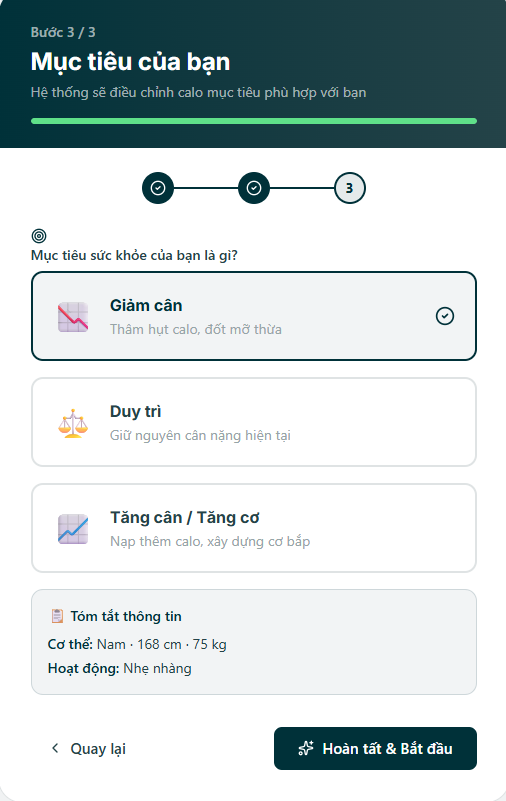
\includegraphics[width=0.32\textwidth]{images/onboarding_step1.png}\hfill
    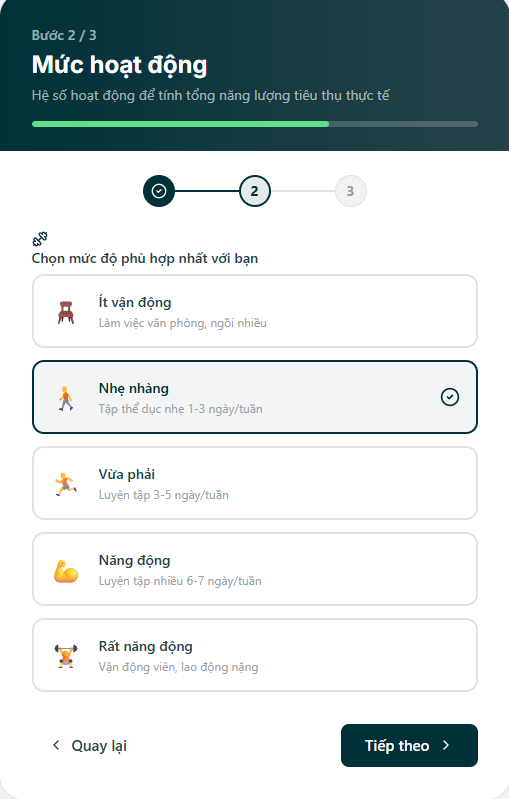
\includegraphics[width=0.32\textwidth]{images/onboarding_step2.png}\hfill
    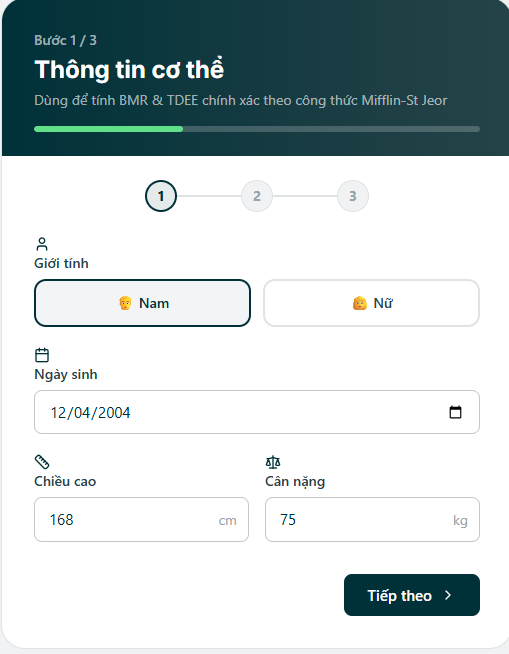
\includegraphics[width=0.32\textwidth]{images/onboarding_step3.png}
    \caption{Màn hình Onboarding / Tính TDEE}
    \label{fig:onboarding}
\end{figure}

Đối với nhóm nhật ký dinh dưỡng và dashboard, kiểm thử được thực hiện bằng cách thêm món ăn vào từng bữa trong ngày, thay đổi khẩu phần và xóa bản ghi đã thêm. Khi một món ăn được ghi nhận, hệ thống lưu khẩu phần, bữa ăn, ngày sử dụng và các giá trị dinh dưỡng tại thời điểm thêm. Cách lưu này giúp dữ liệu nhật ký giữ nguyên giá trị đã ghi nhận, kể cả khi thông tin món ăn trong cơ sở dữ liệu được chỉnh sửa sau đó. Sau khi nhật ký thay đổi, dashboard cần cập nhật lại tổng năng lượng, protein, carbohydrate, chất béo, lượng nước, năng lượng tiêu hao từ luyện tập và các chỉ số cơ thể liên quan. Kết quả kiểm thử cho thấy dữ liệu hiển thị trên dashboard thay đổi tương ứng với các bản ghi đã thêm hoặc xóa trong nhật ký (chi tiết màn hình Nhật ký và Dashboard được minh họa lần lượt trong Hình \ref{fig:nhat_ky_dinh_duong} và Hình \ref{fig:dashboard}).

\begin{figure}[htbp]
    \centering
    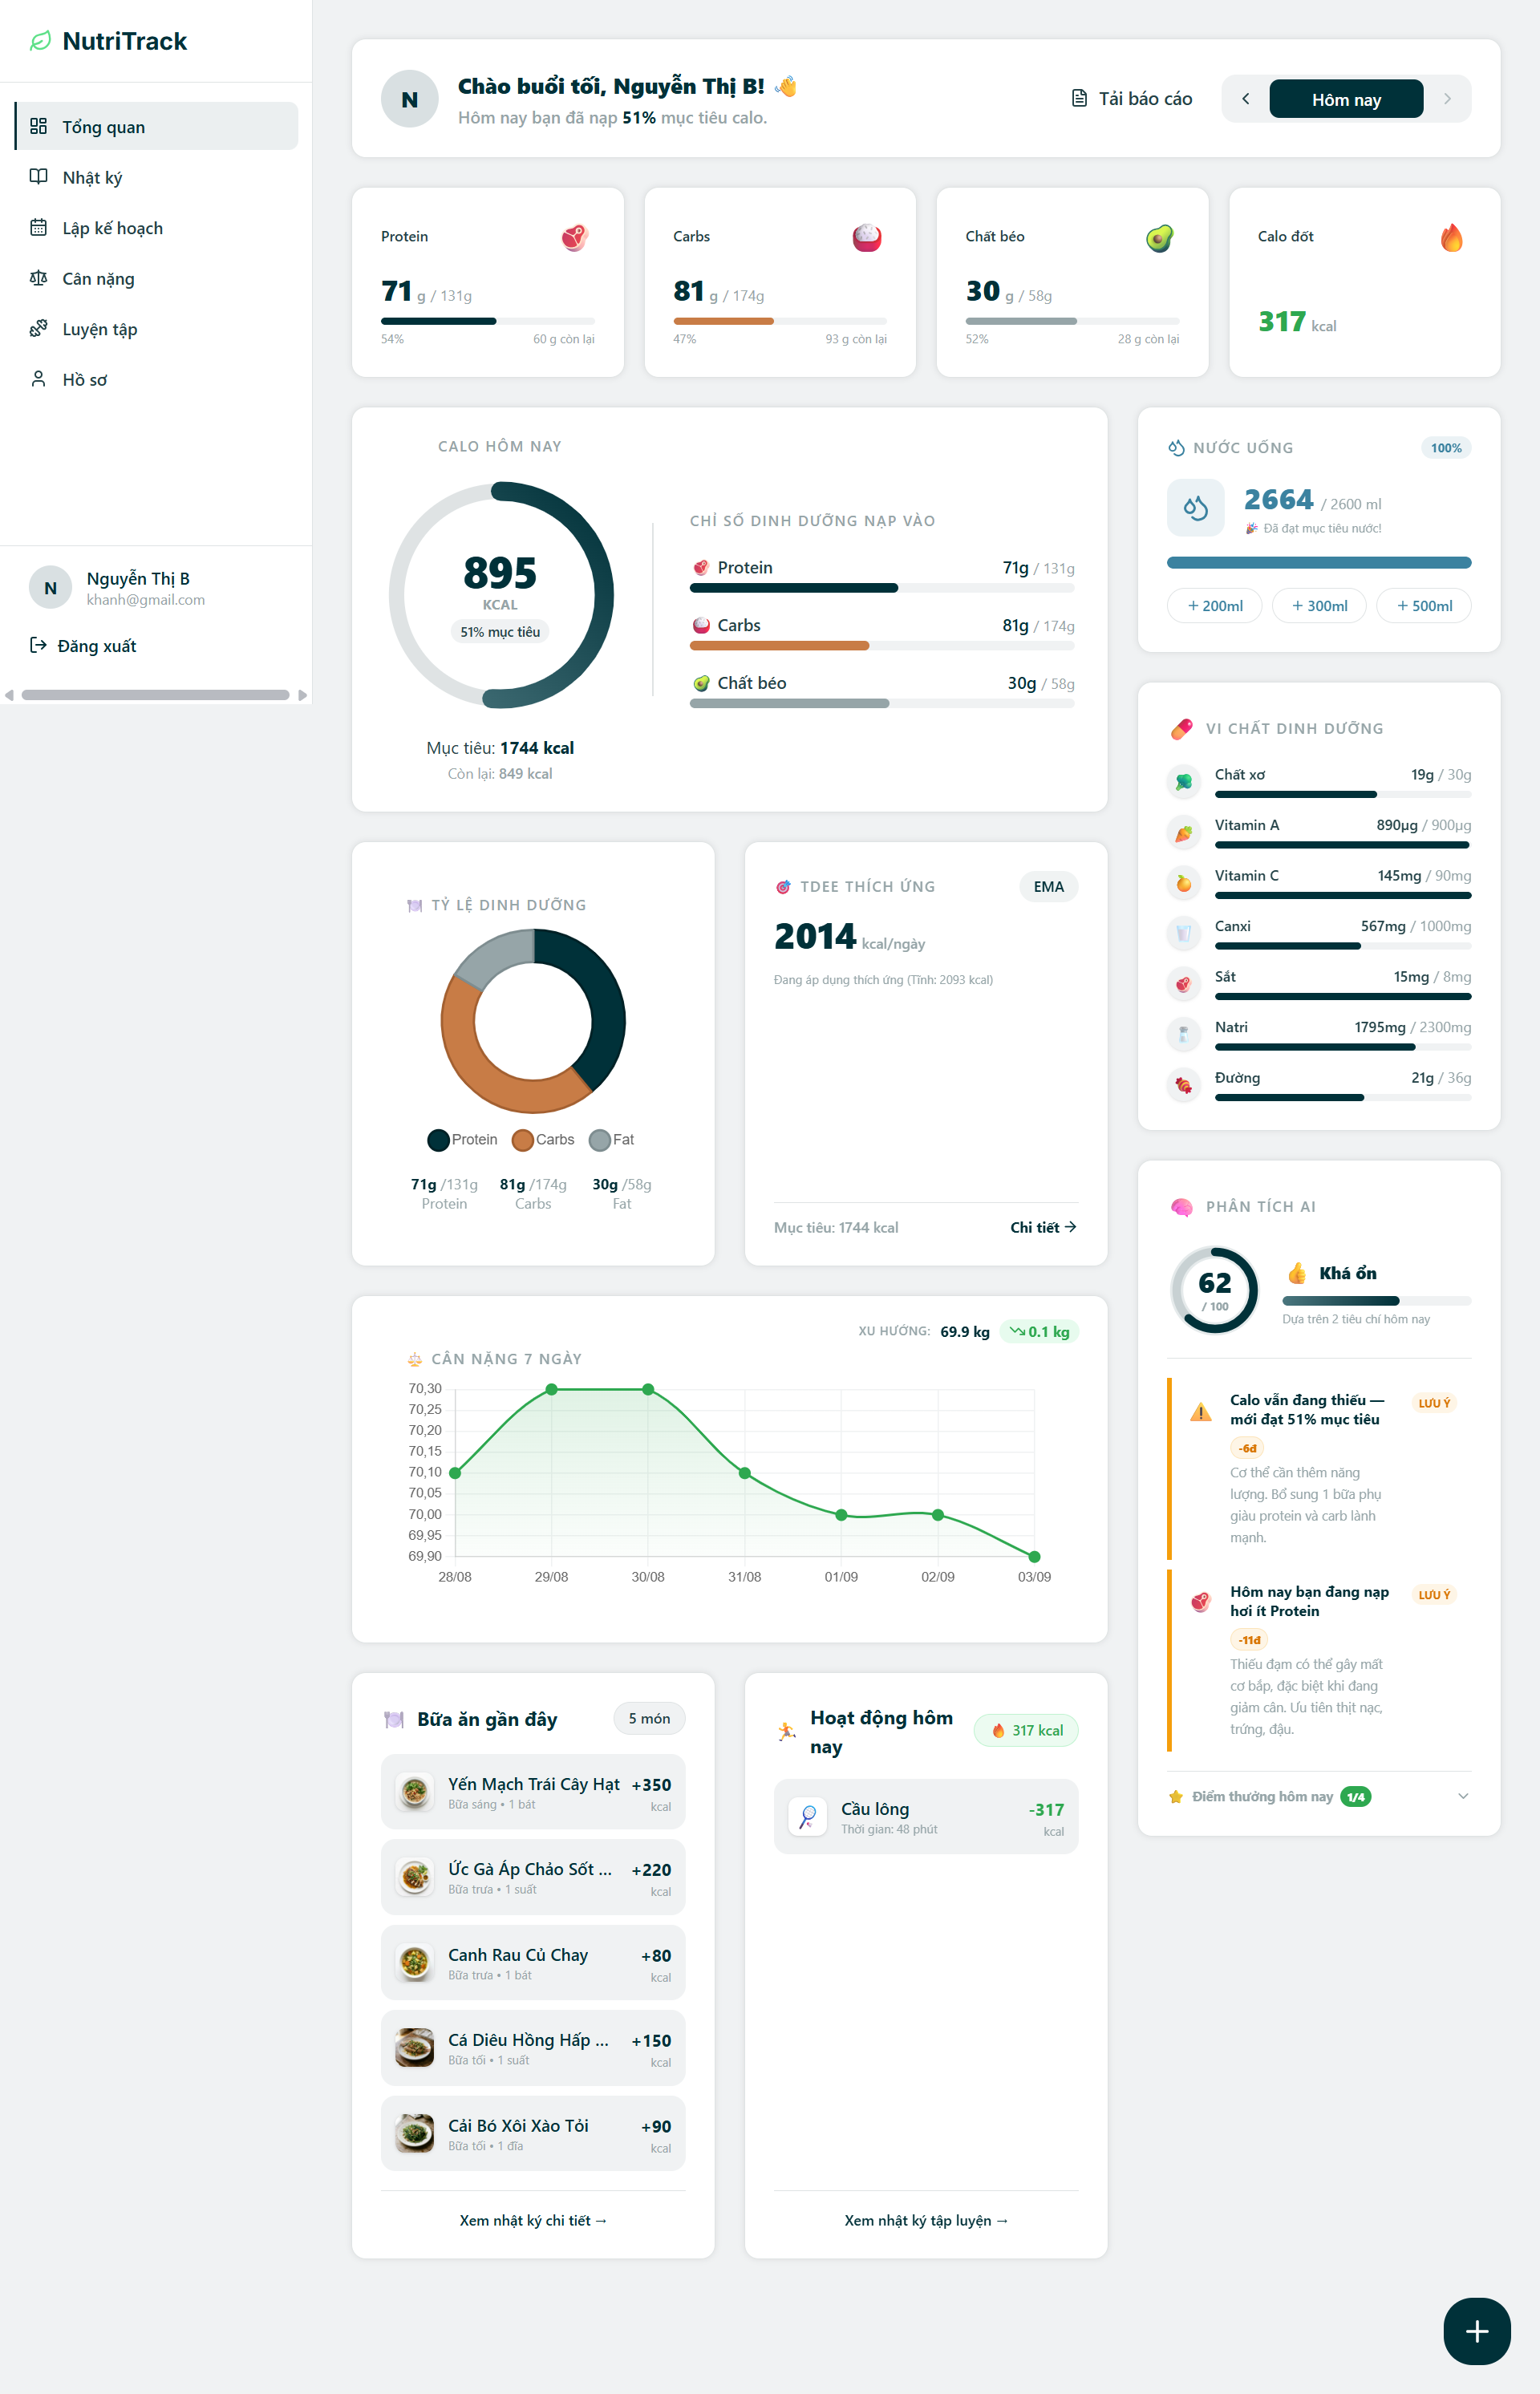
\includegraphics[width=0.85\textwidth]{images/dashboard_overview.png}
    \caption{Màn hình Dashboard (Tổng quan)}
    \label{fig:dashboard}
\end{figure}

\begin{figure}[htbp]
    \centering
    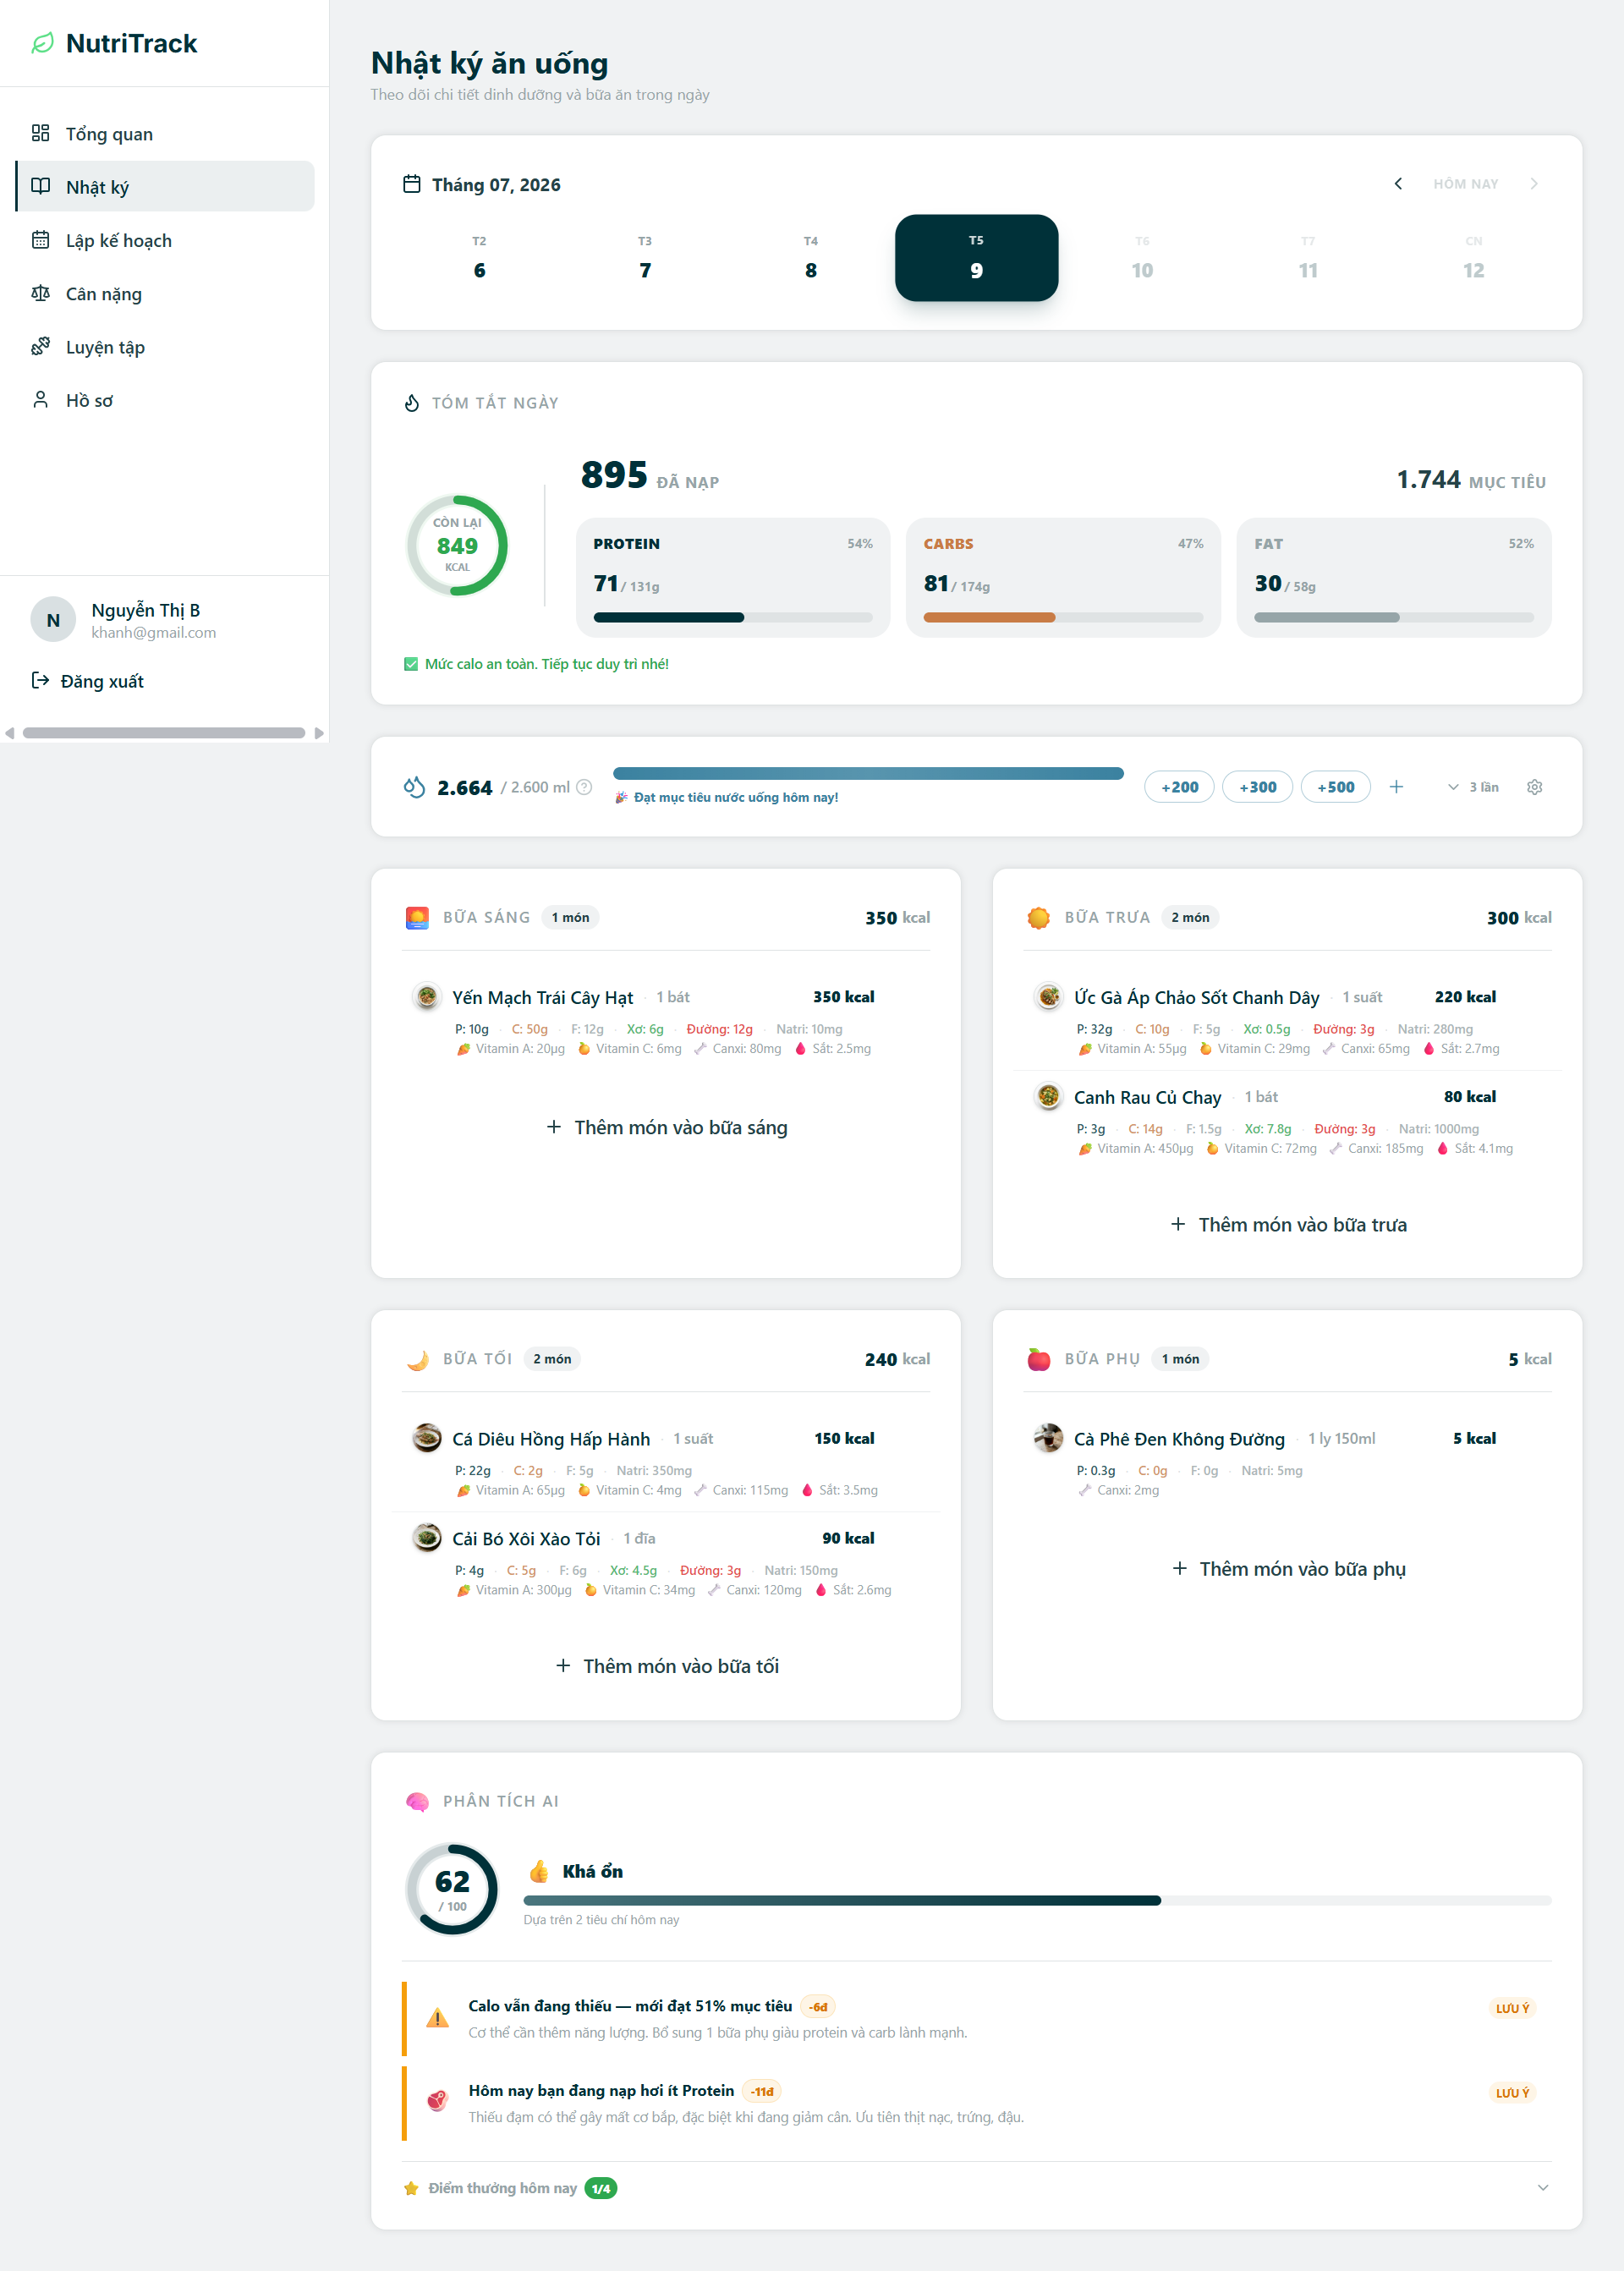
\includegraphics[width=0.85\textwidth]{images/nhat_ky_dinh_duong.png}
    \caption{Màn hình nhật ký dinh dưỡng sau khi thêm món ăn vào bữa trong ngày}
    \label{fig:nhat_ky_dinh_duong}
\end{figure}

Đối với nhóm cân nặng, nước uống và luyện tập, kiểm thử được thực hiện theo các thao tác ghi nhận dữ liệu hằng ngày. Chức năng cân nặng cho phép thêm hoặc cập nhật cân nặng theo ngày, đồng thời đồng bộ cân nặng hiện tại của người dùng theo bản ghi mới nhất. Các trường hợp nhập cân nặng ngoài khoảng cho phép, chọn ngày trong tương lai hoặc nhập giá trị chênh lệch lớn so với xu hướng gần nhất được xử lý bằng thông báo lỗi hoặc yêu cầu xác nhận. Chức năng nước uống cho phép ghi nhận lượng nước theo đơn vị ml và cập nhật mục tiêu nước/ngày. Chức năng luyện tập cho phép chọn môn thể thao, nhập thời lượng và tính năng lượng tiêu hao dựa trên cân nặng người dùng. Sau mỗi thao tác hợp lệ, dữ liệu tổng hợp trong ngày được cập nhật để giao diện hiển thị lại trạng thái mới.

Đối với nhóm Meal Planner, kiểm thử tập trung vào các thao tác lấy cấu hình bữa ăn, cập nhật cấu hình, sinh gợi ý bữa ăn và thay thế nguyên liệu. Kết quả trả về cần có cấu trúc rõ ràng để frontend hiển thị, bao gồm danh sách nguyên liệu, khối lượng hoặc khẩu phần ước tính, tổng năng lượng và các chất dinh dưỡng chính. Trường hợp thay thế nguyên liệu được kiểm tra nhằm bảo đảm hệ thống vẫn trả về một phương án bữa ăn có thể hiển thị sau khi người dùng thay đổi thành phần trong gợi ý ban đầu (xem minh họa trong Hình \ref{fig:meal_planner}).

\begin{figure}[htbp]
    \centering
    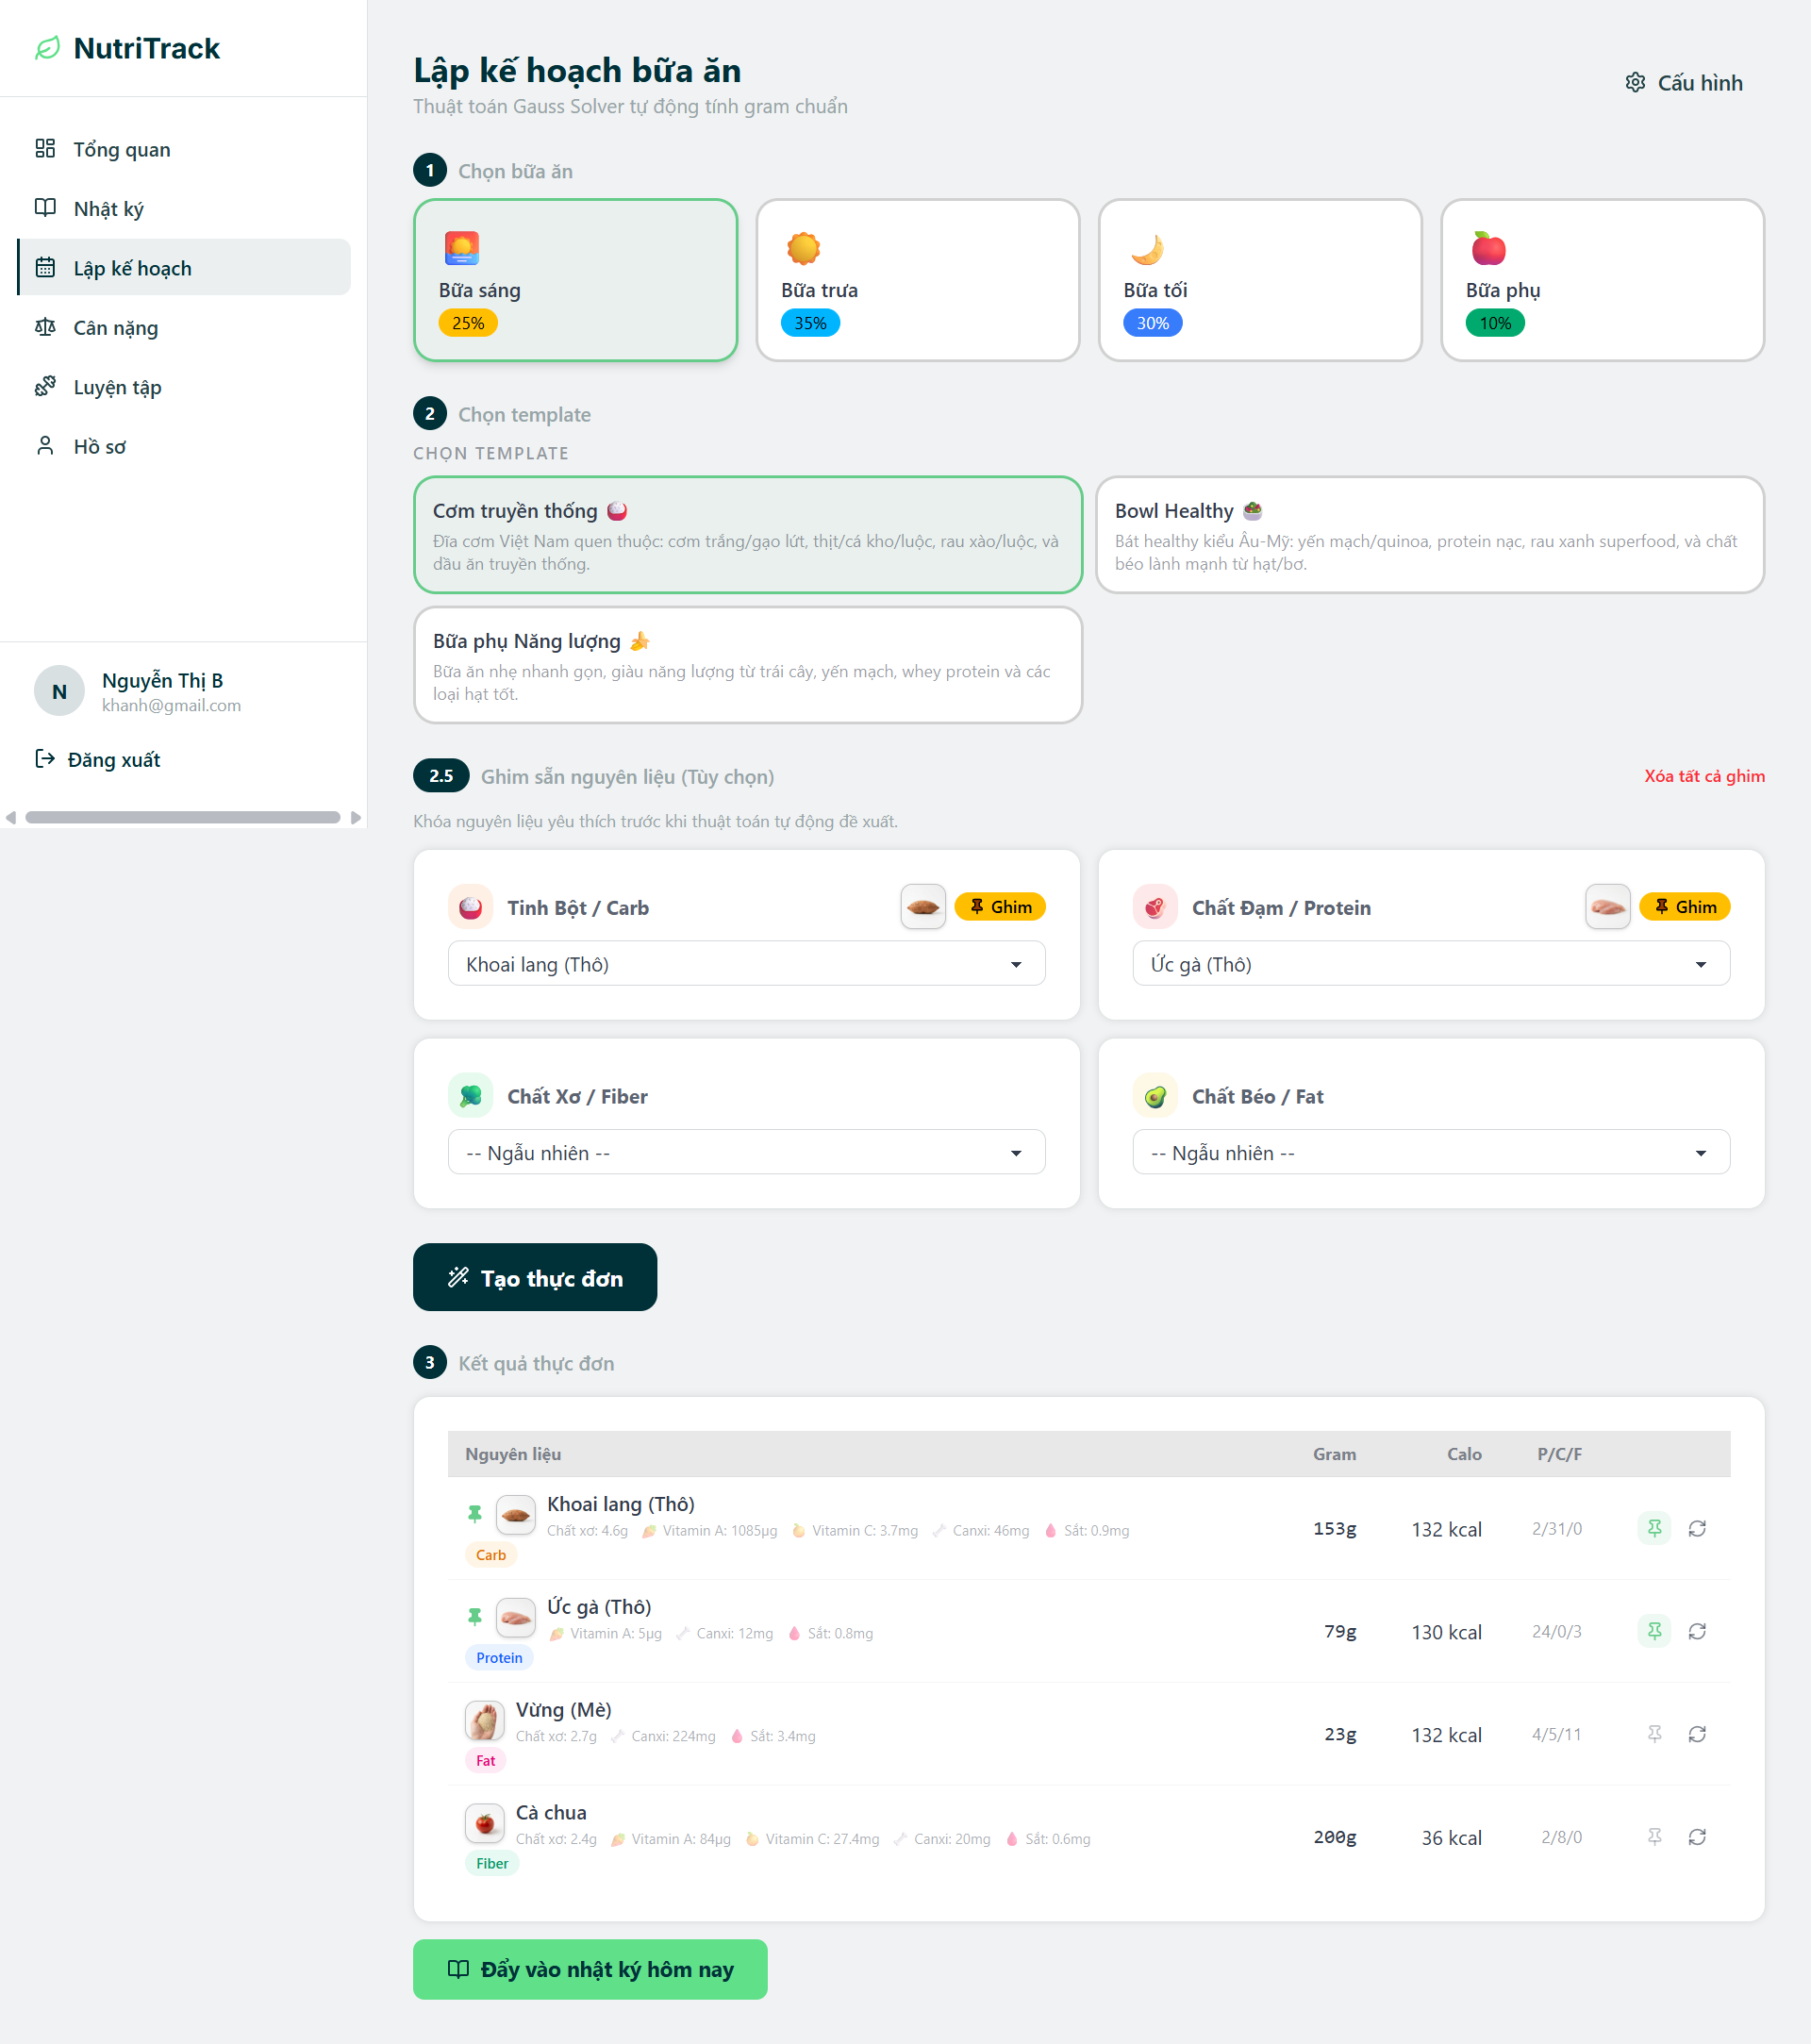
\includegraphics[width=0.85\textwidth]{images/meal_planner.png}
    \caption{Màn hình gợi ý bữa ăn từ chức năng Meal Planner}
    \label{fig:meal_planner}
\end{figure}

Đối với nhóm Hybrid Nutrition Scanner, các trường hợp kiểm thử gồm tra cứu sản phẩm bằng barcode, giải mã barcode từ ảnh, trích xuất thông tin dinh dưỡng từ ảnh, xác nhận đóng góp dữ liệu sản phẩm, tải ảnh sản phẩm và báo cáo dữ liệu sản phẩm sai. Khi dữ liệu ảnh hoặc barcode không đủ điều kiện xử lý, hệ thống trả về thông báo lỗi thay vì ghi nhận dữ liệu chưa được xác nhận. Đối với dữ liệu sản phẩm mới, hệ thống yêu cầu người dùng xác nhận trước khi lưu đóng góp vào cơ sở dữ liệu. Cách xử lý này giúp hạn chế việc lưu các bản ghi sản phẩm thiếu thông tin hoặc chưa đủ độ tin cậy (xem minh họa trong Hình \ref{fig:scanner}).

\begin{figure}[htbp]
    \centering
    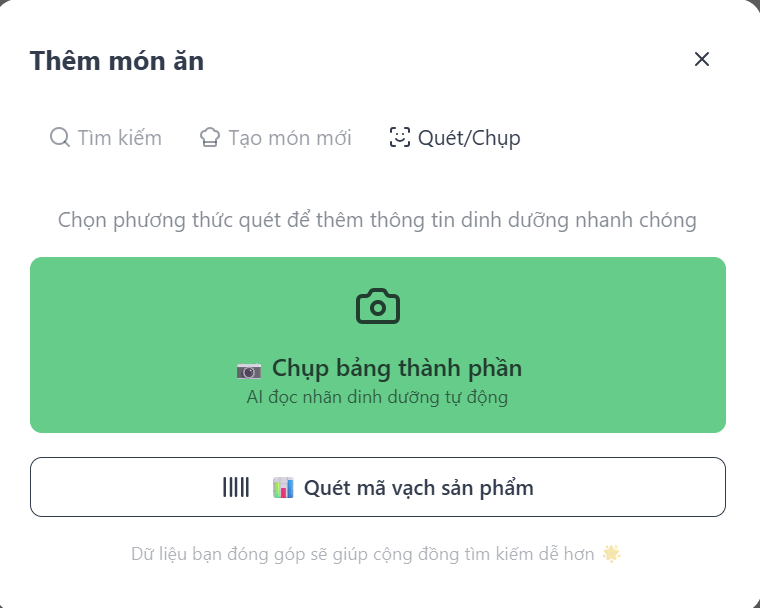
\includegraphics[width=0.48\textwidth]{images/scanner_step1.png}\hfill
    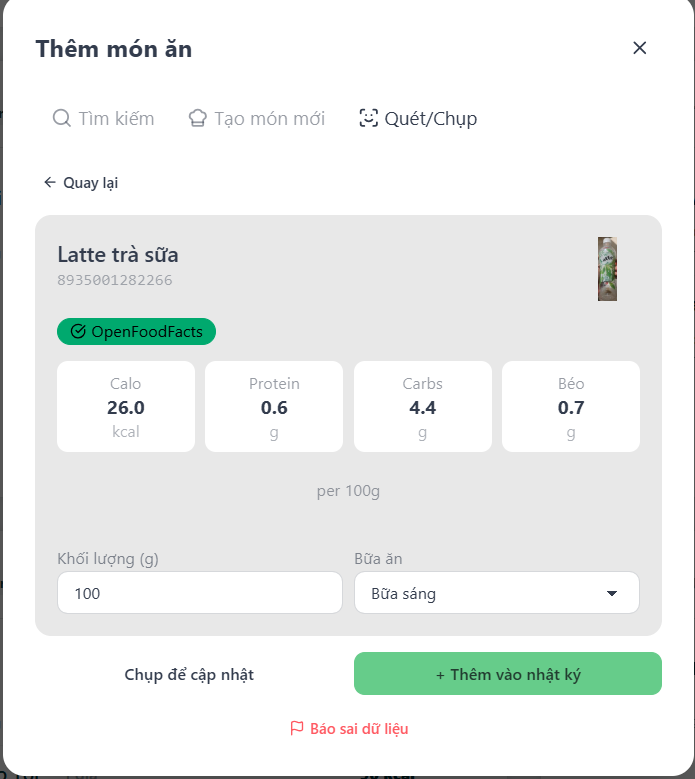
\includegraphics[width=0.48\textwidth]{images/scanner_step2.png}
    \caption{Màn hình Hybrid Nutrition Scanner (Quét đồ ăn bằng AI)}
    \label{fig:scanner}
\end{figure}

Nhìn chung, các nhóm chức năng chính của hệ thống đã đáp ứng được các luồng kiểm thử cơ bản trong phạm vi môi trường cục bộ. Các route yêu cầu đăng nhập chỉ được xử lý khi request có access token hợp lệ. Các thao tác thêm, sửa, xóa dữ liệu được kiểm tra theo phạm vi người dùng hiện tại, qua đó hạn chế truy cập dữ liệu của tài khoản khác. Các lỗi thường gặp như thiếu dữ liệu đầu vào, dữ liệu ngoài khoảng cho phép, token không hợp lệ, endpoint không tồn tại và gửi request vượt giới hạn đều được phản hồi bằng cấu trúc JSON thống nhất. Kết quả kiểm thử chức năng là cơ sở để tiếp tục đánh giá các thuật toán xử lý chính trong mục 4.3. Kết quả kiểm thử các chức năng chính của hệ thống được tổng hợp trong Bảng \ref{tab:kq_kiem_thu_chuc_nang}.

\begin{longtable}{|>{\raggedright\arraybackslash}p{3cm}|>{\raggedright\arraybackslash}p{3cm}|>{\raggedright\arraybackslash}p{4cm}|>{\raggedright\arraybackslash}p{5cm}|}
\caption{Kết quả kiểm thử chức năng chính của hệ thống}
\label{tab:kq_kiem_thu_chuc_nang} \\
\hline
\textbf{Nhóm chức năng} & \textbf{Trường hợp kiểm thử} & \textbf{Kết quả cần đạt} & \textbf{Trạng thái} \\
\hline
\endfirsthead
\hline
\textbf{Nhóm chức năng} & \textbf{Trường hợp kiểm thử} & \textbf{Kết quả cần đạt} & \textbf{Trạng thái} \\
\hline
\endhead

Xác thực tài khoản & Đăng ký và đăng nhập bằng thông tin hợp lệ & Hệ thống trả về thông tin người dùng, access token và thiết lập phiên đăng nhập & Đạt \\
\hline
Xác thực tài khoản & Đăng nhập bằng email hoặc mật khẩu sai & Hệ thống từ chối đăng nhập và trả về thông báo lỗi & Đạt \\
\hline
Bảo vệ API & Gọi API yêu cầu đăng nhập nhưng không gửi access token hợp lệ & Hệ thống không cho phép truy cập tài nguyên được bảo vệ & Đạt \\
\hline
Hồ sơ người dùng & Thiết lập giới tính, ngày sinh, chiều cao, cân nặng, mức độ vận động và mục tiêu & Hồ sơ được lưu, trạng thái onboarding được cập nhật & Đạt \\
\hline
Dashboard & Lấy dữ liệu tổng quan theo ngày & Hệ thống trả về tổng năng lượng, chất dinh dưỡng chính, nước uống, luyện tập và chỉ số liên quan & Đạt \\
\hline
Nhật ký dinh dưỡng & Thêm hoặc xóa món ăn theo ngày, bữa ăn và khẩu phần & Bản ghi được cập nhật, tổng dinh dưỡng trong ngày được tính lại & Đạt \\
\hline
Thực phẩm cá nhân & Tạo, sửa hoặc xóa món ăn do người dùng tự nhập & Hệ thống chỉ xử lý dữ liệu thuộc người dùng hiện tại & Đạt \\
\hline
Nước uống và luyện tập & Ghi nhận lượng nước uống, mục tiêu nước và hoạt động luyện tập & Dữ liệu được lưu, tổng lượng nước hoặc năng lượng tiêu hao được cập nhật & Đạt \\
\hline
Cân nặng & Ghi nhận cân nặng hợp lệ, dữ liệu ngoài khoảng cho phép hoặc ngày trong tương lai & Dữ liệu hợp lệ được lưu; dữ liệu không hợp lệ bị từ chối & Đạt \\
\hline
Meal Planner & Sinh gợi ý bữa ăn và thay thế nguyên liệu & Hệ thống trả về danh sách nguyên liệu, khẩu phần và giá trị dinh dưỡng ước tính & Đạt \\
\hline
Scanner & Tra cứu barcode hoặc xử lý ảnh thông tin dinh dưỡng & Hệ thống trả về thông tin sản phẩm hoặc yêu cầu xác nhận khi dữ liệu chưa đủ chắc chắn & Đạt \\
\hline
Báo cáo PDF & Xuất báo cáo theo khoảng thời gian tuần hoặc tháng & File PDF được sinh từ dữ liệu người dùng và trả về cho trình duyệt & Đạt \\
\hline
Xử lý lỗi & Gửi dữ liệu sai, thiếu token, gọi sai endpoint hoặc gửi request vượt giới hạn & Hệ thống trả về phản hồi lỗi dạng JSON và không ghi dữ liệu không hợp lệ & Đạt \\
\hline
\end{longtable}

\section{Thực nghiệm các thuật toán chính}Bên cạnh kiểm thử chức năng, hệ thống NutriTrack còn được thực nghiệm trên các thuật toán xử lý chính nhằm đánh giá khả năng tính toán và phản hồi theo dữ liệu đầu vào. Phạm vi thực nghiệm tập trung vào các thành phần có ảnh hưởng trực tiếp đến kết quả hiển thị cho người dùng, gồm Nutrition Core, Adaptive TDEE, Food Scoring, Health Insights, Meal Planner và Hybrid Nutrition Scanner. Các thuật toán này không được đánh giá như mô hình học máy, mà được kiểm tra theo hướng thuật toán nghiệp vụ. Theo đó, dữ liệu đầu vào cần được xử lý đúng quy tắc, kết quả trả về cần nhất quán và các trường hợp ngoại lệ cần được kiểm soát.

Dữ liệu thực nghiệm được chuẩn bị theo các tình huống thường gặp trong quá trình sử dụng hệ thống. Với Nutrition Core, dữ liệu đầu vào gồm giới tính, tuổi, chiều cao, cân nặng, mức độ vận động và mục tiêu cá nhân. Với Adaptive TDEE, dữ liệu đầu vào gồm nhật ký năng lượng và cân nặng theo tuần. Với Food Scoring, dữ liệu thực phẩm được kiểm tra theo các chỉ số năng lượng, protein, carbohydrate, chất béo, chất xơ, đường và natri. Với Health Insights, dữ liệu nhật ký trong ngày được dùng để sinh cảnh báo hoặc gợi ý. Với Meal Planner, hệ thống được thử với các mục tiêu năng lượng và macro khác nhau. Với Hybrid Nutrition Scanner, dữ liệu thực nghiệm gồm barcode và ảnh bảng thành phần dinh dưỡng. Kết quả thực nghiệm của các thuật toán chính được trình bày trong Bảng \ref{tab:kq_thuc_nghiem_thuat_toan}.

\begin{longtable}{|>{\raggedright\arraybackslash}p{3cm}|>{\raggedright\arraybackslash}p{3cm}|>{\raggedright\arraybackslash}p{4cm}|>{\raggedright\arraybackslash}p{5cm}|}
\caption{Kết quả thực nghiệm các thuật toán chính}
\label{tab:kq_thuc_nghiem_thuat_toan} \\
\hline
\textbf{Thuật toán} & \textbf{Dữ liệu đầu vào} & \textbf{Kết quả cần kiểm tra} & \textbf{Kết quả thực nghiệm} \\
\hline
\endfirsthead
\hline
\textbf{Thuật toán} & \textbf{Dữ liệu đầu vào} & \textbf{Kết quả cần kiểm tra} & \textbf{Kết quả thực nghiệm} \\
\hline
\endhead

Nutrition Core & Hồ sơ người dùng, mức độ vận động, mục tiêu & Tính BMI, BMR, TDEE, macro và mục tiêu nước & Trả về đủ các chỉ số nền tảng cho Dashboard, Profile, Meal Planner và PDF Report \\
\hline
Adaptive TDEE & Năng lượng nạp vào và cân nặng theo tuần & Ước lượng TDEE từ dữ liệu thực tế & Tính được TDEE theo tuần và có giới hạn khi dữ liệu vượt ngưỡng cho phép \\
\hline
Food Scoring & Năng lượng, protein, carbohydrate, chất béo, chất xơ, đường, natri & Chấm điểm chất lượng món ăn & Điểm thay đổi theo mật độ protein, chất xơ, đường và natri \\
\hline
Health Insights & Tổng năng lượng, macro, nước uống, luyện tập & Sinh cảnh báo hoặc gợi ý theo ngưỡng & Tạo được cảnh báo thiếu nước, thiếu protein, dư năng lượng hoặc mất cân đối macro \\
\hline
Meal Planner & Mục tiêu năng lượng, macro và cấu hình bữa ăn & Sinh khẩu phần phù hợp với mục tiêu & Trả về nguyên liệu, khẩu phần ước tính và tổng dinh dưỡng của bữa ăn \\
\hline
Hybrid Nutrition Scanner & Barcode hoặc ảnh nhãn dinh dưỡng & Trích xuất và chuẩn hóa dữ liệu sản phẩm & Trả về sản phẩm hợp lệ hoặc yêu cầu xác nhận khi dữ liệu chưa đủ điều kiện \\
\hline
\end{longtable}


Đối với Nutrition Core, kết quả kiểm thử được đối chiếu với các giá trị tính toán độc lập từ công thức Mifflin-St Jeor nhằm kiểm tra việc cài đặt công thức BMR trong hệ thống \cite{mifflin1990}. Khi hồ sơ cá nhân được cập nhật, hệ thống tính BMI, BMR, TDEE, năng lượng mục tiêu, tỷ lệ protein, carbohydrate, chất béo và mục tiêu nước. Các giá trị này được sử dụng trong Dashboard để so sánh với dữ liệu ăn uống thực tế, trong Meal Planner để xác định mục tiêu bữa ăn và trong PDF Report để tổng hợp kết quả theo khoảng thời gian. Việc dùng chung một lớp xử lý giúp hạn chế sai khác giữa các màn hình chức năng.

Đối với Adaptive TDEE, thực nghiệm được thực hiện với dữ liệu cân nặng và năng lượng trong nhiều ngày. Một trường hợp kiểm thử sử dụng dữ liệu 7 ngày, trong đó cân nặng giảm từ 80,2 kg xuống 79,5 kg và năng lượng trung bình đạt khoảng 1970 kcal/ngày. Hệ thống ghi nhận TDEE tĩnh là 2500 kcal/ngày, Adaptive TDEE là 2200 kcal/ngày và mức chênh lệch là 300 kcal/ngày, tương ứng 12\%. Kết quả này cho thấy thuật toán có thể phản ánh sự khác biệt giữa công thức tĩnh và dữ liệu thực tế. Ngoài ra, thuật toán có cơ chế giới hạn kết quả trong khoảng cho phép so với TDEE tĩnh nhằm giảm ảnh hưởng của dữ liệu nhập sai.

Đối với Food Scoring và Health Insights, kết quả thực nghiệm cho thấy hệ thống có thể chuyển dữ liệu dinh dưỡng thành điểm số, cảnh báo và gợi ý ngắn gọn. Trong phạm vi dữ liệu thử nghiệm, các món có mật độ protein hoặc chất xơ cao, đồng thời có lượng đường và natri thấp, nhận điểm tốt hơn. Ngược lại, món có nhiều đường, natri hoặc năng lượng cao nhưng ít chất dinh dưỡng có xu hướng bị giảm điểm (xem minh họa màn hình chấm điểm trong Hình \ref{fig:food_scoring}).

\begin{figure}[htbp]
    \centering
    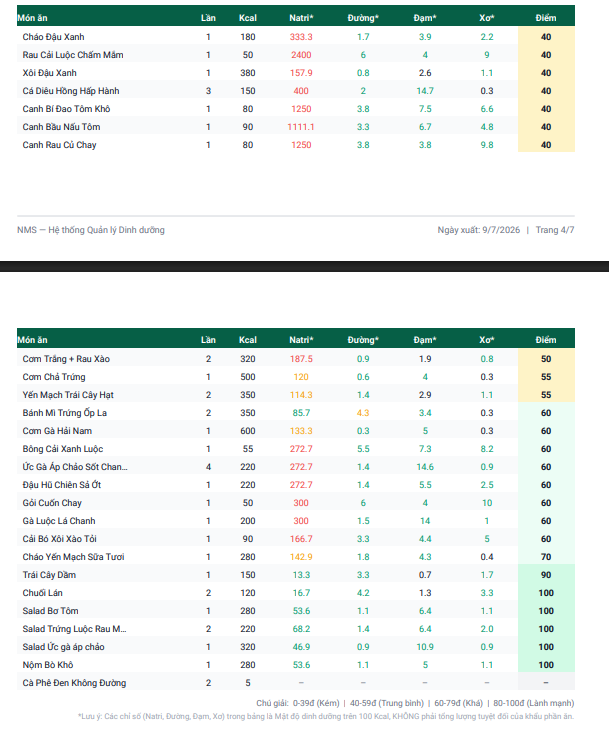
\includegraphics[width=0.85\textwidth]{images/food_scoring.png}
    \caption{Màn hình Food Scoring (Chấm điểm thực phẩm)}
    \label{fig:food_scoring}
\end{figure}

Với Health Insights, khi dữ liệu nhật ký trong ngày thay đổi, danh sách cảnh báo cũng thay đổi theo. Các cảnh báo như thiếu nước, thiếu protein, dư năng lượng hoặc mất cân đối macro được sinh ra dựa trên các ngưỡng điều kiện đã định nghĩa trong backend.

Đối với Meal Planner, thực nghiệm tập trung vào khả năng tạo khẩu phần theo mục tiêu năng lượng và macro của bữa ăn. Hệ thống trả về danh sách nguyên liệu, khối lượng hoặc khẩu phần ước tính, tổng năng lượng và các chất dinh dưỡng chính. Khi tổ hợp nguyên liệu không tạo được kết quả hợp lệ, hệ thống không ghi nhận khẩu phần sai lệch mà trả về thông báo để người dùng thay đổi lựa chọn. Đối với Hybrid Nutrition Scanner, hai luồng chính được kiểm tra gồm tra cứu barcode và nhận dạng ảnh nhãn dinh dưỡng. Khi barcode khớp với dữ liệu đã có, hệ thống trả về thông tin sản phẩm tương ứng. Khi dữ liệu được trích xuất từ ảnh còn thiếu hoặc không đạt điều kiện kiểm tra hợp lệ, hệ thống yêu cầu xác nhận trước khi lưu vào cơ sở dữ liệu.
Nhìn chung, các thuật toán chính đã xử lý được các tình huống dữ liệu cơ bản và trả về kết quả phù hợp với mục tiêu của từng chức năng. Nutrition Core đóng vai trò tính toán nền tảng, Adaptive TDEE hỗ trợ điều chỉnh theo dữ liệu thực tế, Food Scoring đánh giá chất lượng món ăn, Health Insights chuyển dữ liệu thành cảnh báo, Meal Planner tạo khẩu phần theo mục tiêu và Scanner hỗ trợ thu thập dữ liệu thực phẩm. Kết quả thực nghiệm cũng cho thấy chất lượng dữ liệu đầu vào vẫn là yếu tố ảnh hưởng trực tiếp đến kết quả xử lý. Tổng hợp đánh giá kết quả thực nghiệm được thống kê trong Bảng \ref{tab:tong_hop_danh_gia}.

\section{Đánh giá kết quả}Trong phạm vi kiểm thử cục bộ, hệ thống NutriTrack đã đáp ứng được các yêu cầu cơ bản của một hệ thống quản lý dinh dưỡng cá nhân. Các chức năng chính như xác thực tài khoản, quản lý hồ sơ, ghi nhận nhật ký ăn uống, theo dõi cân nặng, nước uống, luyện tập, thống kê dashboard, lập kế hoạch bữa ăn, quét thông tin sản phẩm và xuất báo cáo đều có thể thực hiện theo luồng nghiệp vụ đã thiết kế. Dữ liệu sau khi được thêm, sửa hoặc xóa được cập nhật lại trên các màn hình liên quan, qua đó bảo đảm sự liên kết giữa giao diện, API và cơ sở dữ liệu.

\begin{table}[htbp]
\centering
\caption{Tổng hợp đánh giá kết quả thực nghiệm}
\label{tab:tong_hop_danh_gia}
\begin{tabular}{|>{\raggedright\arraybackslash}p{4cm}|>{\raggedright\arraybackslash}p{4cm}|p{7cm}|}
\hline
\textbf{Tiêu chí đánh giá} & \textbf{Kết quả ghi nhận} & \textbf{Nhận xét} \\
\hline
Tính đầy đủ chức năng & Các nhóm chức năng chính đã được triển khai và kiểm thử & Đáp ứng phạm vi chức năng của đồ án \\
\hline
Tính nhất quán dữ liệu & Dữ liệu nhật ký, dashboard, thuật toán và báo cáo có liên kết với nhau & Hạn chế sai khác giữa các màn hình chức năng \\
\hline
Phản hồi API & API trả về dữ liệu và lỗi theo cấu trúc JSON thống nhất & Thuận lợi cho frontend xử lý và hiển thị \\
\hline
Kết quả thuật toán & Các thuật toán chính trả về kết quả theo dữ liệu đầu vào & Phù hợp với mục tiêu hỗ trợ theo dõi dinh dưỡng cá nhân \\
\hline
Xuất báo cáo & Báo cáo PDF tổng hợp được dữ liệu trong phạm vi 7 ngày và 30 ngày & Phù hợp cho chức năng xem lại quá trình theo dõi \\
\hline
\end{tabular}
\end{table}

\section{Hạn chế và hướng phát triển}Mặc dù hệ thống NutriTrack đã triển khai được các chức năng chính phục vụ quản lý dinh dưỡng cá nhân, kết quả thực nghiệm vẫn còn một số giới hạn cần tiếp tục cải thiện. Trước hết, quá trình kiểm thử mới được thực hiện chủ yếu trên môi trường cục bộ và dữ liệu có kiểm soát, do đó chưa phản ánh đầy đủ tình huống nhiều người dùng truy cập đồng thời trong thời gian dài. Cơ sở dữ liệu thực phẩm đã có các trường dinh dưỡng cơ bản, tuy nhiên số lượng món ăn và sản phẩm đóng gói vẫn phụ thuộc vào dữ liệu nhập sẵn hoặc dữ liệu do người dùng đóng góp. Điều này có thể ảnh hưởng đến kết quả tìm kiếm, chấm điểm món ăn và lập kế hoạch bữa ăn.

Đối với các thuật toán xử lý, Nutrition Core, Adaptive TDEE, Food Scoring, Health Insights và Meal Planner đều phụ thuộc vào độ đầy đủ của dữ liệu đầu vào. Nếu người dùng ghi nhật ký ăn uống không thường xuyên, nhập sai cân nặng hoặc bỏ qua dữ liệu luyện tập, kết quả tổng hợp và các gợi ý có thể bị sai lệch. Riêng Meal Planner đã hỗ trợ loại trừ thực phẩm dị ứng và ghim nguyên liệu khi sinh gợi ý bữa ăn, nhưng kết quả vẫn phụ thuộc vào độ phong phú của dữ liệu nguyên liệu, mẫu bữa ăn và cấu hình bữa ăn. Chức năng Hybrid Nutrition Scanner cũng chịu ảnh hưởng bởi chất lượng ảnh, góc chụp, độ rõ của nhãn sản phẩm và cách trình bày thông tin dinh dưỡng trên bao bì. Vì vậy, kết quả trích xuất từ ảnh cần tiếp tục được kiểm soát bằng bước xác nhận của người dùng. Các hạn chế và hướng phát triển tương ứng của hệ thống được tóm tắt trong Bảng \ref{tab:han_che_huong_phat_trien}.

\begin{longtable}{|>{\raggedright\arraybackslash}p{5cm}|p{10cm}|}
\caption{Hạn chế và hướng phát triển của hệ thống}
\label{tab:han_che_huong_phat_trien} \\
\hline
\textbf{Hạn chế hiện tại} & \textbf{Hướng phát triển} \\
\hline
\endfirsthead
\hline
\textbf{Hạn chế hiện tại} & \textbf{Hướng phát triển} \\
\hline
\endhead

Dữ liệu thực nghiệm chủ yếu được kiểm tra trên môi trường cục bộ & Triển khai thử nghiệm trên môi trường máy chủ và kiểm tra với nhiều tài khoản người dùng \\
\hline
Cơ sở dữ liệu thực phẩm và sản phẩm đóng gói còn phụ thuộc vào dữ liệu nhập sẵn & Mở rộng nguồn dữ liệu thực phẩm và bổ sung cơ chế kiểm duyệt dữ liệu do người dùng đóng góp \\
\hline
Kết quả Adaptive TDEE phụ thuộc vào nhật ký cân nặng và năng lượng nhiều ngày & Bổ sung cơ chế nhắc nhập dữ liệu và đánh giá độ tin cậy của từng giai đoạn theo dõi \\
\hline
Adaptive TDEE hiện chỉ suy ra mức tiêu hao từ năng lượng nạp và biến động cân nặng, chưa có dữ liệu thành phần cơ thể hoặc phép đo năng lượng tiêu hao trực tiếp. Do adaptive thermogenesis được xác định bằng mức chênh lệch giữa tiêu hao đo được và tiêu hao dự đoán sau khi điều chỉnh theo thành phần cơ thể, hệ thống chưa thể xác định trực tiếp hiện tượng này \cite{nunes2022, muller2013}. & Trong hướng phát triển, có thể bổ sung dữ liệu thành phần cơ thể, tăng thời gian quan sát và kiểm định thuật toán trên dữ liệu đo thực nghiệm. \\
\hline
Meal Planner đã có loại trừ dị ứng và ghim nguyên liệu, nhưng còn phụ thuộc vào dữ liệu nguyên liệu và mẫu bữa ăn & Mở rộng mẫu bữa ăn, bổ sung ràng buộc về khẩu vị, ngân sách, thời gian chuẩn bị và mục tiêu theo từng giai đoạn \\
\hline
Scanner phụ thuộc vào chất lượng ảnh, barcode và thông tin trên nhãn sản phẩm & Cải thiện bước kiểm tra dữ liệu sau nhận dạng và quy trình xác nhận trước khi lưu \\
\hline
Báo cáo PDF mới tập trung vào dữ liệu theo tuần và tháng & Bổ sung biểu đồ xu hướng dài hạn và so sánh giữa các giai đoạn theo dõi \\
\hline
\end{longtable}


\section{Kết luận chương}Chương 4 đã trình bày quá trình thực nghiệm và đánh giá hệ thống NutriTrack sau giai đoạn triển khai. Nội dung chương tập trung vào môi trường thực nghiệm, kiểm thử chức năng, thực nghiệm các thuật toán chính, đánh giá kết quả, đồng thời nêu ra một số hạn chế và hướng phát triển tiếp theo. Trong phạm vi kiểm thử cục bộ, các nhóm chức năng chính của hệ thống đã hoạt động theo luồng nghiệp vụ đã thiết kế, bao gồm xác thực tài khoản, quản lý hồ sơ, ghi nhận nhật ký dinh dưỡng, theo dõi nước uống, cân nặng, luyện tập, thống kê dashboard, lập kế hoạch bữa ăn, quét thông tin sản phẩm và xuất báo cáo PDF (Chi tiết xem Bảng \ref{tab:tong_hop_chuong_4}).

\begin{longtable}{|>{\raggedright\arraybackslash}p{5cm}|p{10cm}|}
\caption{Tổng hợp nội dung đánh giá trong Chương 4}
\label{tab:tong_hop_chuong_4} \\
\hline
\textbf{Nội dung đánh giá} & \textbf{Kết quả tổng quát} \\
\hline
\endfirsthead
\hline
\textbf{Nội dung đánh giá} & \textbf{Kết quả tổng quát} \\
\hline
\endhead

Môi trường thực nghiệm & Hệ thống được kiểm thử trên môi trường cục bộ với backend, frontend và cơ sở dữ liệu \\
\hline
Kiểm thử chức năng & Các chức năng chính có thể thực hiện theo luồng người dùng đã xây dựng \\
\hline
Thực nghiệm thuật toán & Các thuật toán chính trả về kết quả theo dữ liệu đầu vào \\
\hline
Xử lý lỗi & API phản hồi lỗi theo cấu trúc JSON thống nhất \\
\hline
Hạn chế & Kết quả còn phụ thuộc vào dữ liệu đầu vào, phạm vi kiểm thử và chất lượng dữ liệu thực phẩm \\
\hline
\end{longtable}

\chapter*{KẾT LUẬN}
\addcontentsline{toc}{chapter}{KẾT LUẬN}
Đồ án đã trình bày quá trình nghiên cứu, phân tích, thiết kế, xây dựng và đánh giá hệ thống NutriTrack, một hệ thống hỗ trợ quản lý dinh dưỡng cá nhân. Xuất phát từ nhu cầu theo dõi năng lượng, thành phần dinh dưỡng và chỉ số cơ thể theo dữ liệu hằng ngày, hệ thống được xây dựng theo mô hình ứng dụng web với backend xử lý nghiệp vụ, frontend cung cấp giao diện tương tác và cơ sở dữ liệu lưu trữ thông tin người dùng, thực phẩm, nhật ký ăn uống, cân nặng, nước uống, luyện tập và báo cáo.

Trong quá trình thực hiện, đồ án đã làm rõ cơ sở lý thuyết liên quan đến quản lý dinh dưỡng cá nhân, bao gồm các khái niệm về năng lượng, protein, carbohydrate, chất béo, chất xơ, đường, natri, BMI, BMR, TDEE và mục tiêu dinh dưỡng. Trên cơ sở đó, hệ thống được phân tích theo các nhóm chức năng chính như quản lý tài khoản, thiết lập hồ sơ người dùng, ghi nhận nhật ký ăn uống, theo dõi chỉ số cơ thể, thống kê dữ liệu dinh dưỡng, đề xuất bữa ăn, quét thông tin sản phẩm và sinh báo cáo. Các chức năng này được tổ chức theo kiến trúc tách biệt giữa tầng giao diện, tầng xử lý nghiệp vụ và tầng dữ liệu.

Về mặt triển khai, hệ thống đã xây dựng được các chức năng cốt lõi phục vụ quá trình theo dõi dinh dưỡng cá nhân. Người dùng có thể đăng ký, đăng nhập, cập nhật hồ sơ, thêm món ăn vào nhật ký, ghi nhận cân nặng, nước uống và hoạt động luyện tập. Dựa trên các dữ liệu này, hệ thống có thể tổng hợp dashboard, tính toán chỉ số nền tảng, đánh giá chất lượng món ăn, đưa ra cảnh báo sức khỏe, lập kế hoạch bữa ăn và xuất báo cáo theo khoảng thời gian. Các thành phần như Nutrition Core, Adaptive TDEE, Food Scoring, Health Insights, Meal Planner và Hybrid Nutrition Scanner được triển khai nhằm hỗ trợ xử lý dữ liệu dinh dưỡng thay vì chỉ lưu trữ thông tin thô.

Trong phạm vi kiểm thử cục bộ, kết quả thực nghiệm cho thấy các nhóm chức năng chính đã hoạt động theo luồng nghiệp vụ đã thiết kế. Các API phản hồi dữ liệu theo cấu trúc JSON thống nhất, các chức năng yêu cầu đăng nhập được bảo vệ bằng cơ chế xác thực, các thao tác thêm, sửa, xóa dữ liệu được kiểm tra theo phạm vi người dùng hiện tại. Bên cạnh đó, các thuật toán xử lý chính cho kết quả phù hợp với dữ liệu đầu vào trong phạm vi kiểm thử. Adaptive TDEE phản ánh sự khác biệt giữa công thức tính tĩnh và dữ liệu thực tế; Food Scoring hỗ trợ đánh giá món ăn theo mật độ dinh dưỡng; Health Insights chuyển dữ liệu nhật ký thành cảnh báo hoặc gợi ý; Meal Planner tạo khẩu phần theo mục tiêu năng lượng và thành phần dinh dưỡng; Hybrid Nutrition Scanner hỗ trợ thu thập thông tin sản phẩm từ barcode hoặc ảnh nhãn dinh dưỡng.

Mặc dù vậy, hệ thống vẫn còn một số hạn chế. Phạm vi kiểm thử chủ yếu được thực hiện trên môi trường cục bộ và dữ liệu có kiểm soát, chưa đánh giá đầy đủ trong điều kiện nhiều người dùng truy cập đồng thời. Cơ sở dữ liệu thực phẩm và sản phẩm đóng gói còn phụ thuộc vào dữ liệu nhập sẵn hoặc dữ liệu do người dùng đóng góp. Kết quả của các chức năng như Adaptive TDEE, Health Insights và Meal Planner phụ thuộc đáng kể vào mức độ đầy đủ và chính xác của nhật ký người dùng. Ngoài ra, chức năng quét thông tin dinh dưỡng từ ảnh vẫn có thể bị ảnh hưởng bởi chất lượng ảnh, góc chụp và cách trình bày nhãn sản phẩm.

Trong hướng phát triển tiếp theo, hệ thống có thể được mở rộng theo một số hướng chính. Thứ nhất, cần bổ sung và kiểm duyệt dữ liệu thực phẩm để tăng độ bao phủ của cơ sở dữ liệu dinh dưỡng. Thứ hai, hệ thống cần được triển khai thử nghiệm trên môi trường máy chủ để đánh giá khả năng vận hành, thời gian phản hồi và mức độ phù hợp khi có nhiều người dùng. Thứ ba, chức năng gợi ý bữa ăn có thể tiếp tục được mở rộng trên cơ sở các ràng buộc đã có như loại trừ thực phẩm dị ứng và ghim nguyên liệu, trong đó tập trung thêm vào khẩu vị, ngân sách, thời gian chuẩn bị, chế độ ăn đặc thù và mục tiêu theo từng giai đoạn. Thứ tư, chức năng báo cáo có thể được bổ sung biểu đồ xu hướng dài hạn, hỗ trợ theo dõi sự thay đổi của cân nặng, năng lượng, macro và thói quen ăn uống qua nhiều tuần hoặc nhiều tháng.

Tổng thể, đồ án đã hoàn thành mục tiêu xây dựng một hệ thống quản lý dinh dưỡng cá nhân có khả năng ghi nhận, tính toán, tổng hợp và đánh giá dữ liệu dựa trên thông tin người dùng cung cấp. Kết quả đạt được cho thấy hệ thống có thể đáp ứng các nghiệp vụ chính của bài toán, đồng thời tạo nền tảng để tiếp tục phát triển các chức năng phân tích và gợi ý dinh dưỡng trong các phiên bản sau.

\clearpage
\pagestyle{empty}
\addtocontents{toc}{\protect\contentsline{chapter}{TÀI LIỆU THAM KHẢO}{}{}}
\renewcommand{\bibname}{\centering TÀI LIỆU THAM KHẢO}

\begin{thebibliography}{9}
\thispagestyle{empty}

\bibitem{vien_dinh_duong_2007}
Viện Dinh dưỡng (2007),
\textit{Bảng thành phần thực phẩm Việt Nam},
Nhà xuất bản Y học, Hà Nội.

\bibitem{mifflin1990}
Mifflin, M. D., St Jeor, S. T., Hill, L. A., et al. (1990).
\textit{A new predictive equation for resting energy expenditure in healthy individuals}.
The American Journal of Clinical Nutrition.
Truy cập ngày 30/06/2026, từ \url{https://pubmed.ncbi.nlm.nih.gov/2305711/}

\bibitem{jankau2025}
Jankau, J., Rogoń, I., Kaczmarek, M., et al. (2025).
"The Challenges of Postoperative Tissue Flap Vitality Monitoring in Obese Individuals".
\textit{Journal of Clinical Medicine}, 14.
Truy cập ngày 11/07/2026, từ \url{https://pmc.ncbi.nlm.nih.gov/articles/PMC12610855/}

\bibitem{fao_who_unu_2001}
FAO/WHO/UNU. (2004).
"Human Energy Requirements: Report of a Joint FAO/WHO/UNU Expert Consultation, Rome, 17–24 October 2001".
\textit{FAO Food and Nutrition Technical Report Series No. 1}.
Rome: Food and Agriculture Organization of the United Nations. Truy cập ngày 11/07/2026, từ \url{https://www.fao.org/4/y5686e/y5686e07.htm}

\bibitem{jensen2014}
Jensen, M. D., Ryan, D. H., Apovian, C. M., et al. (2014),
"2013 AHA/ACC/TOS Guideline for the Management of Overweight and Obesity in Adults",
\textit{Circulation}, Tập 129, Số Suppl. 2, Trang S102--S138.

\bibitem{fao_2003}
Food and Agriculture Organization of the United Nations (2003),
\textit{Food Energy -- Methods of Analysis and Conversion Factors},
FAO Food and Nutrition Paper 77, Rome. Truy cập ngày 11/07/2026, từ \url{https://www.fao.org/4/y5022e/y5022e04.htm}

\bibitem{chow_hall_2008}
Chow, C. C., Hall, K. D. (2008),
"The Dynamics of Human Body Weight Change",
\textit{PLoS Computational Biology}, Tập 4, Số 3, e1000045.

\bibitem{hall2008}
Hall, K. D. (2008),
"What is the required energy deficit per unit weight loss?",
\textit{International Journal of Obesity}, Tập 32, Số 3, Trang 573--576. DOI: 10.1038/sj.ijo.0803720.

\bibitem{hall_chow_2011}
Hall, K. D., Chow, C. C. (2011),
"Estimating changes in free-living energy intake and its confidence interval",
\textit{The American Journal of Clinical Nutrition}, Tập 94, Số 1, Trang 66--74.

\bibitem{hall2011_lancet}
Hall, K. D., Sacks, G., Chandramohan, D., Chow, C. C., Wang, Y. C., Gortmaker, S. L., Swinburn, B. A. (2011),
"Quantification of the effect of energy imbalance on bodyweight",
\textit{The Lancet}, Tập 378, Số 9793, Trang 826--837.

\bibitem{muller2013}
Müller, M. J., Bosy-Westphal, A. (2013),
"Adaptive thermogenesis with weight loss in humans",
\textit{Obesity}, Tập 21, Số 2, Trang 218--228.

\bibitem{nunes2022}
Nunes, C. L., Casanova, N., Francisco, R., Bosy-Westphal, A., Hopkins, M., Sardinha, L. B., Silva, A. M. (2022),
"Does adaptive thermogenesis occur after weight loss in adults? A systematic review",
\textit{British Journal of Nutrition}, Tập 127, Số 3, Trang 451--469.

\bibitem{rosenbaum2010}
Rosenbaum, M., Leibel, R. L. (2010),
"Adaptive thermogenesis in humans",
\textit{International Journal of Obesity}, Tập 34, Số Suppl. 1, Trang S47--S55.

\bibitem{drewnowski2005}
Drewnowski, A. (2005),
"Concept of a nutritious food: toward a nutrient density score",
\textit{The American Journal of Clinical Nutrition}, Tập 82, Số 4, Trang 721--732.

\bibitem{drewnowski2009}
Drewnowski, A. (2009),
"Defining Nutrient Density: Development and Validation of the Nutrient Rich Foods Index",
\textit{Journal of the American College of Nutrition}, Tập 28, Số 4 Suppl., Trang 421S--426S.

\bibitem{drewnowski2019}
Drewnowski, A., Dwyer, J., King, J. C., Weaver, C. M. (2019),
"A proposed nutrient density score that includes food groups and nutrients to better align with dietary guidance",
\textit{Nutrition Reviews}, Tập 77, Số 6, Trang 404--416.

\bibitem{aha_addedsugars}
AHA,
"Added Sugars",
\textit{American Heart Association}, Truy cập ngày 12/07/2026, từ \url{https://www.heart.org/en/healthy-living/healthy-eating/eat-smart/sugar/added-sugars}.

\bibitem{aha_sodium}
AHA,
"How much sodium should I eat per day?",
\textit{American Heart Association}, Truy cập ngày 12/07/2026, từ \url{https://www.heart.org/en/healthy-living/healthy-eating/eat-smart/sodium/how-much-sodium-should-i-eat-per-day}.

\bibitem{fda_addedsugars}
FDA,
"Added Sugars on the New Nutrition Facts Label",
\textit{U.S. Food and Drug Administration}, Truy cập ngày 12/07/2026, từ \url{https://www.fda.gov/food/nutrition-facts-label/added-sugars-nutrition-facts-label}.

\bibitem{mela2018}
Mela, D. J., Woolner, E. M. (2018),
"Perspective: Total, Added, or Free? What Kind of Sugars Should We Be Talking About?",
\textit{Advances in Nutrition}, Tập 9, Số 2, Trang 63--69.

\bibitem{who2015}
WHO (2015),
\textit{Guideline: Sugars intake for adults and children},
World Health Organization, Geneva.

\bibitem{nihNutrientRecommendations}
NIH Office of Dietary Supplements,
``Nutrient Recommendations and Databases'',
\textit{\url{https://ods.od.nih.gov/HealthInformation/nutrientrecommendations.aspx}},
truy cập ngày 14/07/2026.

\bibitem{nihVitaminA}
NIH Office of Dietary Supplements,
``Vitamin A and Carotenoids -- Health Professional Fact Sheet'',
\textit{\url{https://ods.od.nih.gov/factsheets/VitaminA-HealthProfessional/}},
truy cập ngày 14/07/2026.

\bibitem{nihVitaminC}
NIH Office of Dietary Supplements,
``Vitamin C -- Health Professional Fact Sheet'',
\textit{\url{https://ods.od.nih.gov/factsheets/VitaminC-HealthProfessional/}},
truy cập ngày 14/07/2026.

\bibitem{offNutritionData}
Open Food Facts, ``Explain nutrition data'',
\textit{\url{https://openfoodfacts.github.io/openfoodfacts-server/dev/explain-nutrition-data/}},
truy cập ngày 14/07/2026.

\bibitem{offApiCheatSheet}
Open Food Facts, ``Reference: API CheatSheet'',
\textit{\url{https://openfoodfacts.github.io/openfoodfacts-server/api/ref-cheatsheet/}},
truy cập ngày 14/07/2026.

\bibitem{googleGeminiGenerateContent}
Google AI for Developers, ``Generating content'',
\textit{\url{https://ai.google.dev/api/generate-content}},
truy cập ngày 14/07/2026.

\bibitem{googleGemini25Flash}
Google AI for Developers, ``Gemini 2.5 Flash'',
\textit{\url{https://ai.google.dev/gemini-api/docs/models/gemini-2.5-flash}},
truy cập ngày 14/07/2026.

\end{thebibliography}
\end{document}